\documentclass[hyper,linkcolor=blue]{mythesis}

\usepackage[colorinlistoftodos]{todonotes}
\makeatother

\title{Discovery and measurement of the Higgs boson in the \WW decay channel}
\author{David Christopher Hall}


\begin{document}
%TC:ignore
\begin{frontmatter}
  %!TEX root = ../thesis.tex

%% Title
\titlepage[\vspace{12pt}St Catherine's College, University of Oxford]{
\vspace{-160pt}
\begin{figure}[ht]
	\null\hfill
	\includegraphics[height=4.5cm,clip=true,trim=0 1.4cm 0 0]{tex/catz-arms.pdf}
	\hfill
	\includegraphics[height=4.5cm]{tex/ox-logo.pdf}
	\hfill\null
\end{figure}
\vspace{4pt}
Submitted in partial fulfilment of the requirements\\ 
for the degree of Doctor of Philosophy\\
Trinity 2014}

%% Abstract
\begin{abstract}%[\smaller \thetitle\\ \vspace*{1cm} \smaller {\theauthor}]
  %\thispagestyle{empty}
  %!TEX root = ../thesis.tex

\todo[inline]{Write abstract}

\end{abstract}

%% Preface
\begin{preface}
  %!TEX root = ../thesis.tex

What I personally contributed.
\end{preface}

%% Acknowledgements
\begin{acknowledgements}
  %!TEX root = ../thesis.tex

HSG3 convenors: Jianming, Biagio, Pierre, Tatsuya, Christian, Corrinne
HSG3 members: Jonathan, Christian, Carsten, Sara, et al
HSG3 theory: Justin, Bob
WW convenors: Marc-Andre, Matthias
WW members: Shu, Yusheng
HXSWG

\end{acknowledgements}

%% Quote
\frontquote%
{By believing passionately in something that still does not exist, we create it. \\The nonexistant is whatever we have not sufficiently desired.}
{Franz Kafka}

%% ToC
\setcounter{tocdepth}{1}
\tableofcontents

\end{frontmatter}
%TC:endignore

\begin{mainmatter}
  \cleardoublepage
  \pagenumbering{arabic}
  \listoftodos
  
  \chapter*{Introduction}
    \addcontentsline{toc}{chapter}{Introduction}
    \label{chap:intro}
    %!TEX root = ../thesis.tex

The Standard Model of particle physics describes the behaviour of sub-atomic particles. 
Since its formulation in the 1970s, it has experienced unparalleled success in modelling a 
wide range of phenomena; no experimental result is currently considered to significantly 
contradict its validity.\footnote{
	Observation of neutrino oscillations required neutrino masses to be manually added to 
	the Standard Model. It is widely believed that their relatively small masses will be 
	explained by new physics.
}
However, there are a number of physical phenomena that the Standard Model is unable to 
describe: gravitational attraction between massive objects, the observed asymmetry between 
matter and antimatter in the Universe, and astronomical evidence for dark matter and the 
cosmological constant.

A crucial aspect of the Standard Model is how non-zero masses are imparted to fundamental 
particles. These are forbidden by underlying symmetries of the theory, though remain an 
experimental fact; for example, atoms could not form if the electron did not posses mass.
This is achieved via interactions with a ubiquitous Higgs field, excitations of which 
correspond to Higgs bosons. As the only undiscovered particle of the Standard Model, the 
discovery of the Higgs boson is of utmost importance to the field: it would complete our 
knowledge of the Standard Model, and in particular confirm the mechanism of mass generation. 
As such, it was a primary goal of the LHC physics program, which began in 2010.

This thesis describes the search, discovery and measurement of the Higgs boson using 
proton-proton collision data recorded by the ATLAS experiment at CERN. This is accomplished 
by searching for collisions where a Higgs boson is produced and subsequently decays to two 
\PW bosons, each of which decay to an electron or muon and a neutrino (\ie \HWWlvlv). This 
search suffers from large experimental backgrounds, such as continuum \WW production, which 
must be accurately modelled to yield sensitivity to the Higgs boson.

First, the theoretical motivation for the Higgs boson is presented in 
\Chapter~\ref{chap:motivation}. Then, \Chapter~\ref{chap:tools} outlines some important 
concepts related to making precise predictions within the Standard Model, which shall be 
referred to throughout the thesis. The experimental setup of the LHC and the ATLAS detector 
are described in \Chapter~\ref{chap:experiment}.

Focus then moves to the data analysis itself. \Chapter~\ref{chap:selection} offers an 
overview of the entire \HWW analysis, detailing the selection of Higgs boson signal events 
and the rejection of backgrounds. Following this, signal modelling is described in 
\Chapter~\ref{chap:signal}, \WW background modelling is described in \Chapter~\ref{chap:ww} 
(including a dedicated cross section measurement), and the modelling of other backgrounds is 
described in \Chapter~\ref{chap:backgrounds}. The experimental results are presented and 
discussed in \Chapter~\ref{chap:results}. Finally, in \Chapter~\ref{chap:conclusions}, we 
draw conclusions from the results of this analysis and of others conducted simultaneously at 
the LHC, and consider the outlook of Higgs physics.


\todo[inline]{Each figure/table needs placement specifier (removes weird gaps in text)}


  \chapter{Theoretical motivation}
    \label{chap:motivation}
    %!TEX root = ../../thesis.tex

The Standard Model (SM) of particle physics is the theory of sub-atomic particles.
It is the culmination of many decades of progress in both experimental and theoretical
quantum physics during the 20th century. It has enjoyed unparalleled success in describing 
a wide range of phenomena, which have been experimentally verified to an extraordinary 
degree of precision.

A crucial aspect of the SM is the generation of non-zero particle masses, which are 
forbidden by underlying symmetries of the theory but remain an experimental fact. 
They are generated by 
the Higgs mechanism of electroweak symmetry breaking, which also predicts the existence of 
a massive scalar particle, the Higgs boson, whose mass is a free parameter of the theory. 
As the only undiscovered particle of the SM, the discovery of the Higgs boson was 
a primary goal of the LHC physics program, which began in 2010.

A brief introduction to the SM is given in \Section~\ref{sec:sm}, outlining the 
particle content and interactions of the theory. In \Section~\ref{sec:ewsb}, electroweak 
symmetry breaking is described in detail. Then, some properties of the Higgs boson are 
described in \Section~\ref{sec:properties}, and the constraints upon its mass prior to the 
LHC are detailed in \Section~\ref{sec:prior_constraints}.

    \section{The Standard Model of particle physics}
      \label{sec:sm}
      %!TEX root = ../../thesis.tex

The Standard Model of particle physics (SM) is a quantum field theory describing
the kinematics and interactions of sub-atomic particles. The dynamics of such a 
theory are determined by the symmetries respected by the Lagrangian density.
The SM is invariant under local transformations of the \SMgroup gauge group,
resulting in the strong, weak and electromagnetic forces of nature and determining
the particle content of the theory. Additionally, invariance under global 
transformations of the Poincaré group ensures the theory is identical in all 
inertial frames of reference, as asserted by special relativity.

Each gauge theory of the SM describes the dynamics of a force of nature, which 
is mediated by a number of gauge bosons and couples to a conserved current, in 
accordance with Noether's theorem. Quantum chromodynamics (QCD) describes the strong 
interaction, is mediated by eight gluons and couples to colour charge. Quantum 
electrodynamics (QED) describes the electromagnetic interaction, is mediated by the 
photon and couples to electric charge. The weak interaction is mediated by the massive 
\PWpm and \PZzero bosons and is understood within the context of electroweak theory (EW),
a unification of the electromagnetic and weak interactions. A quantum field theory of
gravity is not included in the SM. It is important to note that the gauge groups of the
strong and weak interactions are non-abelian. Physically, this means that the
gauge bosons are themselves charged and therefore experience self-interactions.

\begin{figure}
	\includegraphics[width=\largefigwidth]{tex/motivation/sm_particles}
	\caption{The particle content of the Standard Model. Mass data from \cite{PDG}.}
	\label{fig:sm_particles}
\end{figure}

The elementary particles of the SM are summarised in \Figure~\ref{fig:sm_particles}.
They are naturally separated into bosons (integer spin) and fermions (half-integer spin).
In addition to the gauge bosons previously introduced, the Higgs boson is a by-product
of electroweak symmetry breaking (described in \Section~\ref{sec:ewsb}) and its
couplings are proportional to mass. The fermions are categorised according to the
interactions they experience, or equivalently the charges they posses: quarks
(strong, electromagnetic, weak), charged leptons (electromagnetic, weak) and neutrinos 
(weak). Most particles also have an associated antiparticle with identical mass
but inverted internal quantum numbers.

    \section{Electroweak unification}
      \label{sec:ewsb}
      %!TEX root = ../../thesis.tex

The first theory of weak interactions was a four-point interaction with Fermi coupling 
constant \unit{$G_F = 1.166\times 10^{-5}$}{\GeV\rpsquared}. Although successful in 
describing low energy phenomena, such as nuclear $\beta$-decay and muon decay, at 
energies above \unit{\about300}{\GeV} the theory predicted cross sections which violate 
unitarity \cite{Aitchison}.

The solution was to introduce charged vector bosons (\PWpm bosons) to mediate the weak 
interaction, similar to the exchange of photons in \ac{QED}. However, unlike \ac{QED}, 
the weak interaction is short ranged and therefore its exchange bosons must be massive. 
Since the propagator for a particle of mass $m$ and momentum $p$ contains 
$1 / (p^2 - m^2)$, in the low energy limit we can relate to Fermi's theory and identify
\begin{equation}
	G_F \sim g^2 / m_{\PW}^2
\end{equation}
where $g$ is the coupling of the vector boson. Thus, at low energies, the strength of the weak interaction is suppressed by the mass of the exchange boson.

At this time, there were two key obstacles to unifying the electromagnetic and weak 
interactions. Firstly, the discovery of parity violation in cobalt-60 $\beta$-decay 
implied the weak interaction has a \VminusA structure, whereas \ac{QED} has a pure V 
structure \cite{Wu:1957}.\footnote{
	Five bilinear covariants can be constructed from the Dirac $\gamma$ matrices, which 
	are named according to how they transform under parity: scalar, pseudoscalar, vector, 
	axial vector and tensor.
}
Secondly, the \PWpm bosons are massive whilst photons are massless. This was a major problem because gauge bosons are inherently massless.\footnote{
	Consider the gauge transformation of a Yang-Mills gauge field 
	$\bvec{W}_{\mu} \rightarrow \bvec{W}_{\mu} - \partial_{\mu} \bvec{\alpha}(x)
	- g \lbrack \bvec{\alpha}(x) \times \bvec{W}_{\mu} \rbrack$. Clearly the mass term 
	$-\tfrac{1}{2}m^2 \bvec{W}_{\mu} \cdot \bvec{W}^{\mu}$ is not gauge invariant, and 
	hence the gauge boson is massless.}
In fact, fermion masses were also forbidden by the chiral nature of the weak interaction, 
but were known to exist.\footnote{
	Consider a spinor as the sum of its left- and right-handed chiral states 
	$\psi = \psi_L + \psi_R$. Then the Dirac mass term is $-m \bar{\psi} \psi = 
	-m (\bar{\psi}_R \psi_L + \bar{\psi}_L \psi_R)$. For a chiral theory, $\psi_L$ and
	$\psi_R$ behave differently under gauge transformations and thus the mass term is not gauge invariant.
}

Glashow's proposal of an \EWgroup group was a major step forward \cite{Glashow:1961}. 
This model describes three gauge fields \rowthreevec{W^1_{\mu}}{W^2_{\mu}}{W^3_{\mu}} 
which couple to weak isospin $T$ with strength $g$, and a single gauge field $B_{\mu}$ 
which couples to weak hypercharge $Y$ with strength $g'$. The subscript $L$ indicates 
that only left-handed chiral particles couple to the $W^i_{\mu}$ fields, explaining the 
\VminusA nature of the weak interaction whilst preserving \ac{QED}. The physical gauge 
fields are obtained through the mixing of these fields
\begin{align}
	W^{\pm}_{\mu} &= (W^1_{\mu} \mp i W^2_{\mu}) / \sqrt{2} \label{eq:Wfield} \\
	Z_{\mu} &= \cos\theta_W W^3_{\mu} - \sin\theta_W B_{\mu} \label{eq:Zfield} \\
	A_{\mu} &= \sin\theta_W W^3_{\mu} + \cos\theta_W B_{\mu} \label{eq:Afield}
\end{align}
where
\begin{align}
	\cos\theta_W = g/\sqrt{g^2 + g'^2} && \sin\theta_W = g'/\sqrt{g^2 + g'^2} \,. \label{eq:weak_mixing}
\end{align}
We identify $W^{\pm}_{\mu}$ with the \PWpm bosons, $A_{\mu}$ with the photon 
and $Z_{\mu}$ with a new neutral \PZ boson. Weak neutral currents were later confirmed 
experimentally \cite{Gargamelle:1973}. 

Glashow's \EWgroup theory therefore predicts the interaction of fermions, in left-handed 
\SUgroup{2} doublets and right-handed \SUgroup{2} singlets (see 
\Table~\ref{tab:ew_fermions}), with \PWpm, \PZ and \Pphoton 
exchange bosons. Gauge boson self-interactions are also expected due to the non-abelian 
nature of the \ac{EW} theory. The \PWpm bosons couple to weak isospin $T$ with strength 
$g$, the \PZ boson couples vectorially to $c_V$ and axially to $c_A$ with strength 
$g/(2\cos\theta_W)$, and the photon couples to electric charge $Q$ with strength 
$e = g\sin\theta_W$, where
\begin{align}
	c_V &= T_3 - 2 Q \sin^2\theta_W \quad\quad c_A = T_3 \\
	Q   &= T_3 + \frac{Y}{2} \,.
\end{align}

\begin{table}[b]
	\begin{tabular}{ccc@{\hskip 1cm}cccc}
		& & & $T$ & $T_3$ & $Y$ & $Q$ \\
		\hline
		\multirow{2}{*}{$\colvector{\Pnue\\ \Pe}_{\!\!\!L}$} & 
		\multirow{2}{*}{$\colvector{\Pnum\\ \Pmu}_{\!\!\!L}$} & 
		\multirow{2}{*}{$\colvector{\Pnut\\ \Ptau}_{\!\!\!L}$} & 
		$\tfrac{1}{2}$ & $+\tfrac{1}{2}$ & $-1$ & 0 \\
		& & & $\tfrac{1}{2}$ & $-\tfrac{1}{2}$ & $-1$ & $-1$ \\
		$\Pnue_R$ & $\Pnum_R$ & $\Pnut_R$ & 0 & 0 & 0 & 0 \\
		$\Pe_R$ & $\Pmu_R$ & $\Ptau_R$ & 0 & 0 & $-2$ & $-1$ \\
		\hline
		\multirow{2}{*}{$\colvector{\Pup\\ \Pdown'}_{\!\!\!L}$} & 
		\multirow{2}{*}{$\colvector{\Pcharm\\ \Pstrange'}_{\!\!\!L}$} & 
		\multirow{2}{*}{$\colvector{\Ptop\\ \Pbottom'}_{\!\!\!L}$} & 
		$\tfrac{1}{2}$ & $+\tfrac{1}{2}$ & $+\tfrac{1}{3}$ & $+\tfrac{2}{3}$ \\
		& & & $\tfrac{1}{2}$ & $-\tfrac{1}{2}$ & $+\tfrac{1}{3}$ & $-\tfrac{1}{3}$ \\
		$\Pup_R$ & $\Pcharm_R$ & $\Ptop_R$ & 0 & 0 & $+\tfrac{4}{3}$ & $+\tfrac{2}{3}$ \\
		$\Pdown'_R$ & $\Pstrange'_R$ & $\Pbottom'_R$ & 0 & 0 & $-\tfrac{2}{3}$ & $-\tfrac{1}{3}$ \\
	\end{tabular}
	\caption{The weak isospin $T$, weak hypercharge $Y$ and electric charge $Q$ quantum
	numbers assigned to the fermions. Right-handed neutrinos are decoupled from the 
	electroweak interaction, and were not originally included in the \ac{SM}. However, 
	recent observations of neutrino oscillations suggest these might exist.}
	\label{tab:ew_fermions}
\end{table}

Unfortunately, it was necessary to explicitly break the symmetry by adding mass terms for 
the \PWpm and \PZ bosons by hand. Initial attempts to invoke a mechanism of \ac{SSB} were 
hindered by the Goldstone theorem.



\subsection{The Goldstone theorem}
\label{sec:ewsb:goldstone}
\ac{SSB} arises when the vacuum state does not respect the symmetry in question. This can 
occur when a field acquires a non-zero vacuum expectation value. To see this, consider a 
complex scalar field $\phi$ described by the Lagrangian
\begin{equation}
	\mathcal{L} 
	= \parenths{\partial_{\mu}\phi^{\dagger}} \parenths{\partial^{\mu}\phi} 
	+ \mu^2 \phi^{\dagger}\phi - \lambda \parenths{\phi^{\dagger}\phi}^2
	\label{eq:lagr:goldstone}
\end{equation}
with positive $\mu^2$ and $\lambda$, giving a sombrero potential 
(\Figure~\ref{fig:sombrero}). 
Although $\mathcal{L}$ is invariant under global \Ugroup{1} transformations 
$\phi \rightarrow \eexp{-i\alpha} \phi$, there are infinite degenerate vacua
$\phi = \mu\eexp{-i\theta}/\sqrt{2\lambda}$ that are not invariant. In order to interact 
with the system, a single vacuum must be arbitrarily chosen, spontaneously breaking the 
\Ugroup{1} symmetry.

\begin{figure}[b]
	\includegraphics[width=\mediumfigwidth]{tex/motivation/sombrero}
	\caption{The sombrero potential, in which a vacuum state must be arbitrarily chosen, 
	spontaneously breaking the symmetry of the underlying Lagrangian.
	Fluctuations in the azimuthal direction correspond to a massless Nambu-Goldstone 
	boson. Fluctuations in the radial direction correspond to a massive Higgs boson.}
	\label{fig:sombrero}
\end{figure}

The Goldstone theorem states that \ac{SSB} of a continuous global symmetry will lead to 
the existence of a number of massless scalar Nambu-Goldstone bosons \cite{Goldstone:1962}.
This can be seen by considering radial and azimuthal excitations, $h\parenths{x}$ and 
$\theta\parenths{x}$, about the vacuum 
\begin{equation}
	\phi\parenths{x} = \frac{1}{\sqrt{2}} \sqbracs{v + h\parenths{x}} \eexp{-i\theta\parenths{x} / v}
\end{equation}
where $v = \mu/\sqrt{\lambda}$. When substituted into (\ref{eq:lagr:goldstone}), we get
\begin{equation}
	\mathcal{L} = \tfrac{1}{2}\partial_{\mu}\theta \partial^{\mu}\theta
	+ \tfrac{1}{2}\partial_{\mu}h \partial^{\mu}h
	- \mu^2 h^2
	+ \dots
\end{equation}
where the dots denote terms neither kinetic nor mass. 
We identify a massless Nambu-Goldstone boson (the $\theta$-mode) and a Higgs boson of 
mass $\sqrt{2}\mu$ (the $h$-mode).

In order to explain massive \PWpm and \PZ bosons, the electroweak symmetry must be broken.
But the Goldstone theorem suggested that this would predict massless scalar bosons, which
were not experimentally observed.



\subsection{The Higgs mechanism}
\label{sec:ewsb:higgs}
However, when \ac{SSB} of a continuous \textit{local} symmetry is studied, something 
remarkable happens. The Nambu-Goldstone bosons of the theory are `eaten' by the gauge 
bosons, giving them mass. The associated degrees of freedom appear as longitudinal 
components of the massive gauge bosons. This is known as the Higgs mechanism 
\cite{Englert:1964,Higgs:1964a,Higgs:1964b,Guralnik:1964,Higgs:1966}.

Consider the Lagrangian for a \Ugroup{1} gauge theory with a sombrero potential
\begin{equation}
	\mathcal{L} 
	= \parenths{D_{\mu}\phi}^{\dagger} \parenths{D^{\mu}\phi}
	- \tfrac{1}{4} F_{\mu\nu} F^{\mu\nu}
	+ \mu^2 \phi^{\dagger} \phi - \lambda \parenths{\phi^{\dagger} \phi}^2
	\label{eq:lagr:abelHiggs}
\end{equation}
where $D_{\mu} = \partial_{\mu} + iqA_{\mu}$ is the covariant derivative and $F_{\mu\nu} 
= \partial_{\mu}A_{\nu} - \partial_{\nu}A_{\mu}$ is the field tensor. This is invariant 
under local \Ugroup{1} transformations $\phi \rightarrow \eexp{-i\alpha\parenths{x}} \phi$
when accompanied by a gauge transformation of the potential 
$A_{\mu} \rightarrow A_{\mu} + \tfrac{1}{q}\partial_{\mu} \alpha\parenths{x}$.

We are free to choose the unitary gauge $\alpha\parenths{x} = -\theta\parenths{x}/v$,
altering the photon field $A_{\mu} \rightarrow A_{\mu} - \tfrac{1}{qv}\partial_{\mu} 
\theta\parenths{x}$ in the process. Ultimately, the final result is gauge-independent, 
but other choices make the gauge boson propagators gauge-dependent. Since the 
$\theta$-mode is `gauged away', excitations about the vacuum become
\begin{equation}
	\phi\parenths{x} = \frac{1}{\sqrt{2}} \sqbracs{v + h\parenths{x}}
\end{equation}
and the Lagrangian (\ref{eq:lagr:abelHiggs}) becomes
\begin{equation}
	\mathcal{L}
	= \frac{1}{2} q^2 v^2 A_{\mu} A^{\mu}
	- F_{\mu\nu}F^{\mu\nu}
	+ \frac{1}{2} \partial_{\mu}h \partial^{\mu}h
	- \mu^2 h^2
	+ \dots
\end{equation}
where the dots denote terms neither kinetic nor mass. 
The Nambu-Goldstone boson is no longer present and the photon has acquired a mass $qv$.
Again, there is a massive scalar Higgs boson as a by-product of the \ac{SSB}.



\subsection{Glashow-Salam-Weinberg electroweak theory}
The Higgs mechanism can be extended to non-abelian gauge theories, as was necessary to 
describe electroweak symmetry breaking \cite{Kibble:1967,Weinberg:1967,Salam:1968}.
Consider the Lagrangian for an \SUgroup{2}\cross\Ugroup{1} gauge theory with a sombrero
potential
\begin{equation}
	\mathcal{L} 
	= \parenths{D_{\mu}\phi}^{\dagger} \parenths{D^{\mu}\phi}
	- \tfrac{1}{4} \bvec{F}_{\mu\nu} \cdot \bvec{F}^{\mu\nu}
	- \tfrac{1}{4} G_{\mu\nu} G^{\mu\nu}
	+ \mu^2 \phi^{\dagger} \phi - \lambda \parenths{\phi^{\dagger} \phi}^2
	\label{eq:lagr:ewHiggs}
\end{equation}
where $D_{\mu} = \partial_{\mu} + \tfrac{i}{2} g \bvec{\tau} \cdot \bvec{W}_{\mu} + 
\tfrac{i}{2} g' Y B_{\mu}$ is the covariant derivative, and $\bvec{F}_{\mu\nu} = 
\partial_{\mu}\bvec{W}_{\nu} - \partial_{\nu}\bvec{W}_{\mu} - g \bvec{W}_{\mu} \cross 
\bvec{W}_{\nu}$ and $G_{\mu\nu} = \partial_{\mu}B_{\nu} - \partial_{\nu}B_{\mu}$ are the
field tensors. In this case, $\phi$ is an \SUgroup{2} doublet of complex scalar fields
\begin{equation}
	\phi = \colvector{\phi^+\\\phi^0} = \colvector{\frac{1}{\sqrt{2}} \parenths{\phi_1 + i\phi_2}\\ \frac{1}{\sqrt{2}} \parenths{\phi_3 + i\phi_4}}.
\end{equation}

Again, there are infinite degenerate vacua satisfying 
$\parenths{\phi_1^2 + \phi_2^2 + \phi_3^2 + \phi_4^2} = \mu^2/\lambda$. In analogue with 
the abelian Higgs mechanism, the unitary gauge sets the vacuum expectation values of 
$\phi_1$, $\phi_2$ and $\phi_4$ to be zero. Considering excitations about the vacuum
\begin{equation}
	\phi\parenths{x} = \colvector{0\\ \frac{1}{\sqrt{2}} 
	\sqbracs{v + h\parenths{x}}} \label{eq:higgs_doublet}
\end{equation}
the Lagrangian (\ref{eq:lagr:ewHiggs}) becomes
\begin{align}
	\mathcal{L} &= \tfrac{1}{8} g^2 v^2 \bvec{W}_{\mu} \cdot \bvec{W}^{\mu} - \tfrac{1}{4} \bvec{F}_{\mu\nu} \cdot \bvec{F}^{\mu\nu} + \tfrac{1}{8} v^2 g'^2 B_{\mu} B^{\mu} - \tfrac{1}{4} v^2 gg' B_{\mu} W_{3}^{\mu} - \tfrac{1}{4} G_{\mu\nu} G^{\mu\nu} \nonumber \\
	&\quad\quad {} + \tfrac{1}{2} \partial_{\mu}h \partial^{\mu}h - \mu^2 h^2 + \dots \\
	&= \tfrac{1}{4} g^2 v^2 W^{+}_{\mu} W^{-\mu} - \tfrac{1}{2} \parenths{\partial_{\mu}W^{+}_{\nu} - \partial_{\nu}W^{+}_{\mu}} \parenths{\partial^{\mu}W^{-\nu} - \partial^{\nu}W^{-\mu}} \nonumber \\
	&\quad\quad {} + \tfrac{1}{8} v^2 \parenths{g^2 + g'^2} Z_{\mu} Z^{\mu} - \tfrac{1}{4} \parenths{\partial_{\mu}Z_{\nu} - \partial_{\nu}Z_{\mu}} \parenths{\partial^{\mu}Z^{\nu} - \partial^{\nu}Z^{\mu}} - \tfrac{1}{4} F_{\mu\nu} F^{\mu\nu} \nonumber \\
	&\quad\quad {} + \tfrac{1}{2} \partial_{\mu}h \partial^{\mu}h - \mu^2 h^2 + \dots
\end{align}
where the dots denote terms neither kinetic nor mass, and the expression has been rewritten in terms of the physical gauge fields using (\ref{eq:Wfield}), (\ref{eq:Zfield})
and (\ref{eq:Afield}). The \PWpm bosons acquire a mass $gv/2$ and the \PZ boson acquires a
mass $v \sqrt{\parenths{g^2+g'^2}}/2$, while the photon is massless. Again, all Nambu-Goldstone bosons are gone and a Higgs boson has appeared as a by-product of the \ac{SSB}.

This theory predicts a striking relation between the gauge boson masses, using 
(\ref{eq:weak_mixing})
\begin{equation}
	m_{\PW} = m_{\PZ} \cos\theta_W
\end{equation}
which was experimentally verified once the \PW and \PZ bosons were discovered 
\cite{UA1:1989}. It also predicted a massive scalar Higgs boson, whose mass could not be 
determined from the other parameters of the theory.

Fermion masses can also be incorporated into \ac{EW} theory through Yukawa couplings.
Consider a coupling between the electron-type \SUgroup{2} doublet (see 
\Table~\ref{tab:ew_fermions}), the Higgs doublet $\phi$ given in 
(\ref{eq:higgs_doublet}), and the electron \SUgroup{2} singlet
\begin{align}
	\mathcal{L}_{\Pe}^{\text{Yuk}} &= -g_{\Pe} \parenths{\Plepton_{\Pe L} \phi \Pe_{R} + \Pe_{R} \phi^{\dagger} \Plepton_{\Pe L}} \\
	&= -\frac{g_{\Pe}}{\sqrt{2}} \sqbracs{v + h} \parenths{\Pe_{L} \Pe_{R} + \Pe_{R} \Pe_{L}}
\end{align}
where $g_e$ is the electron Yukawa coupling. The electron has acquired a mass 
$g_{\Pe}v/\sqrt{2}$ and the coupling of the Higgs boson to the electron is proportional 
to that mass.

Finally, we note a similar phenomenon in superconductors. There, the \Ugroup{1} symmetry 
of \ac{QED} is spontaneously broken, as in \Section~\ref{sec:ewsb:higgs}, giving mass to 
the photon and thereby producing the Meissner effect. In fact, Higgs bosons have been 
observed in the Raman spectra of superconductors \cite{Superconductivity}. However, a 
major difference is that the bosonic field is a Bose-Einstein condensate of loosely bound 
electron pairs (known as Cooper pairs), and therefore the \ac{SSB} is dynamic. This is 
only possible due to lattice vibrations of the underlying solid. It is natural to ask 
whether a similar dynamic mechanism could be used to break \ac{EW} symmetry, where the 
Higgs boson is a composite particle. This is an active area of theoretical research, 
though will not be explored here.

    \section{Properties of the Higgs boson}
      \label{sec:properties}
      %!TEX root = ../../thesis.tex

The Higgs boson is predicted to have zero spin and positive parity, whilst being 
electrically neutral and colourless. It couples only to massive particles. Other 
properties, such as production cross sections and \acp{BR} of decay, must be calculated 
as a function of its mass, which is not predicted by the \ac{SM}.

% Experimental signatures for the Higgs boson are categorised according to production 
% mode and decay channel.

At a hadron collider such as the \acs{LHC}, the important production modes are \ac{ggF},
\ac{VBF}, Higgs-strahlung (\WH and \ZH) and top fusion (\ttH). Example Feynman diagrams 
are shown in \Figure~\ref{fig:feyn}. We note that the Higgs boson does not couple to 
massless gluons, therefore \ac{ggF} proceeds via loops of massive coloured particles 
(predominantly the top quark due to its large mass). 

\begin{figure}[b]
	\null\hfill
	\begin{subfigure}[b]{0.4\textwidth}
		\centering
		\includegraphics[width=\textwidth]{axodraw/ggF.pdf}
		\caption{Gluon-gluon fusion (ggF)}
		\label{fig:feyn:ggF}
	\end{subfigure}
	\hfill
	\begin{subfigure}[b]{0.4\textwidth}
		\centering
		\includegraphics[width=0.75\textwidth]{axodraw/VBF.pdf}
		\caption{Vector boson fusion (VBF)}
		\label{fig:feyn:VBF}
	\end{subfigure}
	\hfill\null
	\\\bigskip
	\null\hfill
	\begin{subfigure}[b]{0.4\textwidth}
		\centering
		\includegraphics[width=0.8\textwidth]{axodraw/VH.pdf}
		\caption{Higgs-strahlung (\WH and \ZH)}
		\label{fig:feyn:VH}
	\end{subfigure}
	\hfill
	\begin{subfigure}[b]{0.4\textwidth}
		\centering
		\includegraphics[width=0.625\textwidth]{axodraw/ttH.pdf}
		\caption{Top fusion (\ttH)}
		\label{fig:feyn:ttH}
	\end{subfigure}
	\hfill\null
	\caption{Examples of tree-level Feynman diagrams for the Higgs production processes relevant at the \ac{LHC}.}
	\label{fig:feyn}
\end{figure}

The production cross sections at the \acs{LHC} are shown in \Figure~\ref{fig:higgs_xs}. 
Whilst \ac{ggF} clearly dominates these rare processes, it suffers from large 
experimental backgrounds. The four other modes feature additional final state particles 
which can aid identification. For example, \ac{VBF} has two back-to-back quarks with no 
colour exchange between them.

\begin{figure}
	\includegraphics[width=0.48\textwidth]{tex/motivation/xs_lowrange}
	\hfill
	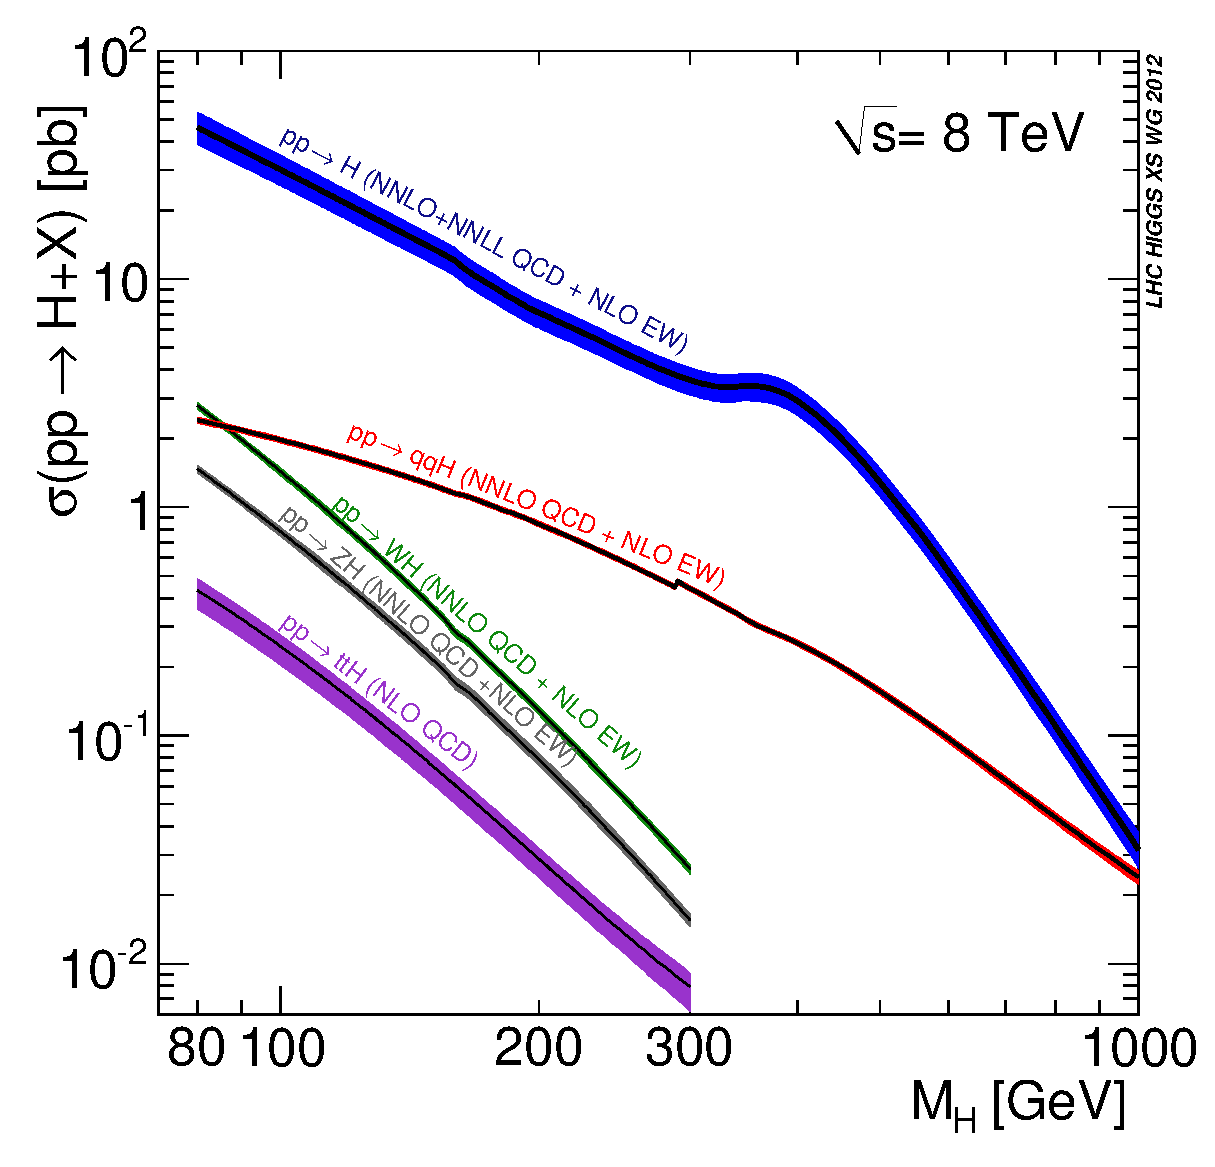
\includegraphics[width=0.48\textwidth]{tex/motivation/xs_fullrange}
	\caption{Higgs boson production cross sections versus mass at 
	\unit{$\sqrt{s} = 8$}{\TeV} for a low mass range (left) and an expanded mass range 
	(right) \cite{YR2}. Theoretical uncertainties are shown as bands. The production modes
	are \ac{ggF} (blue), \ac{VBF} (red), \WH (green), \ZH (grey) and \ttH (purple).}
	\label{fig:higgs_xs}
\end{figure}

Since the lifetime of the Higgs boson is very short, it is never directly observed in a 
detector. Therefore it is important to understand the \acp{BR} of its decays 
(\Figure~\ref{fig:higgs_br}). Na\"{i}vely, these are understood from the Higgs boson coupling to mass and the kinematic requirement $m_H > m_X + m_Y$ for a decay
\HepProcess{\PHiggs \HepTo XY}. This is complicated by off-shell particles (\eg a low mass
Higgs boson may decay to \HepProcess{\PW \PW^{*}}). 
Also, the \HepProcess{\Pphoton \Pphoton}, \HepProcess{\PZ \Pphoton} and 
\HepProcess{\Pgluon \Pgluon} decay modes are different since they feature massless 
particles, and therefore proceed via loops of massive charged particles (electric charge 
for \HepProcess{\Pphoton \Pphoton} and \HepProcess{\PZ \Pphoton}, colour charge for 
\HepProcess{\Pgluon \Pgluon}).

Designing a sensitive experimental search strategy for the Higgs boson can be difficult. 
In decay channels featuring weak bosons, the subsequent decay of the \PW or \PZ must also 
be considered. These are more likely to decay to quarks than leptons, but the former 
suffers from large backgrounds at hadron colliders. Similarly, the 
\HepProcess{\Pbottom \APbottom} has the largest \ac{BR} for low \mH but suffers from huge 
backgrounds. The sensitivity can be improved by combining with a more distinguished 
production mode, such as \WH or \ZH, but this reduces the production cross section.

\begin{figure}
	\includegraphics[width=0.48\textwidth]{tex/motivation/BR_lowrange}
	\hfill
	\includegraphics[width=0.48\textwidth]{tex/motivation/BR_fullrange}
	\caption{Branching ratios of Higgs boson decay versus mass for a low mass range (left) 
	and an expanded mass range (right) \cite{YR3}. Theoretical uncertainties are shown as 
	bands.}
	\label{fig:higgs_br}
\end{figure}

    \section{Pre-LHC constraints on the Higgs boson mass}
      \label{sec:prior_constraints}
      %!TEX root = ../../thesis.tex

\subsection{Direct searches}

\subsection{Electroweak fits}

  \chapter{Computational techniques for the LHC}
    \label{chap:tools}
    %!TEX root = ../../thesis.tex

Although the search for the Higgs boson is motivated by the electroweak interaction, a
detailed knowledge of quantum chromodynamics (QCD) is required to make precise predictions 
at a hadron collider such as the LHC. However, these calculations are troublesome; QCD 
describes the interactions of quarks and gluons, though only the composite hadrons are 
experimentally observed.

Some key concepts of QCD are introduced in \Section~\ref{sec:qcd}, before the 
simulation of LHC collisions is described in \Section~\ref{sec:mc}. Finally, jets are 
introduced in \Section~\ref{sec:jets} as useful tools connecting theoretical calculations 
with experimental observations.

    \section{Quantum chromodynamics}
      \label{sec:qcd}
      %!TEX root = ../../thesis.tex

\ac{QCD} is the theory of the strong interaction, describing coloured particles (quarks 
and gluons, collectively known as partons) \cite{Ellis:1996}. Two crucial features of 
\ac{QCD} are \textit{confinement} and \textit{asymptotic freedom}. Confinement refers to 
the observation that quarks and gluons are only found within colourless hadrons, and 
never as isolated states. Asymptotic freedom states that, within the hadron, the 
constituent partons are relatively free to move. Both concepts can be understood in terms 
of a running coupling constant.



\subsection{Renormalisation and the running coupling constant}
\label{sec:qcd:renormalisation}

When calculating observables within perturbative quantum field theory, ultraviolet (UV) 
divergences are often introduced by Feynman diagrams containing loops. Through careful 
consideration, these UV divergences can be absorbed into renormalised definitions of the 
coupling constant and particle masses. The idea is that the `bare' quantities contain 
compensating divergences, such that the physically measurable quantities are finite:
\begin{equation}
	g_{\text{physical}} = g_{\text{bare}} + \delta g
	\quad\quad\text{and}\quad\quad
	m_{\text{physical}} = m_{\text{bare}} + \delta m
\end{equation}
where $\delta g$ and $\delta m$ are the loop contributions. This procedure is known as 
\textit{renormalisation}.

It is necessary to introduce an unphysical \textit{renormalisation scale} \mur, above 
which loops are absorbed into renormalised quantities, and below which loops are 
calculated in perturbation theory. Clearly couplings and masses will depend upon \mur,
though physical observables must not -- however, truncation of the perturbative series 
will result in a residual \mur dependence. Usually \mur is chosen to be the energy 
scale $Q$ of the process under consideration, leading to the concept of a \textit{running 
coupling constant}.

The \ac{QCD} coupling constant \alphaS is shown in \Figure~\ref{fig:qcd:alpha_s}. At low 
scales (large distances), \alphaS is large and the theory is non-perturbative. 
Though not analytically proven\footnote{
	A mathematically rigorous proof of confinement is one of seven Millennium Prize 
	Problems of the Clay Mathematics Institute, with a bounty of \$1,000,000.
}, confinement has been verified in this regime by lattice \ac{QCD} \cite{Wilson:1974}. 
At high scales (small distances), \alphaS is small -- this is asymptotic freedom 
\cite{Gross:1973,Politzer:1973}. Note that \alphaEM in \acs{QED} exhibits an opposing 
trend, though remains perturbative at all accessible energies.
\begin{figure}
	\includegraphics[width=\mediumfigwidth]{tex/tools/alpha_s}
	\caption{The running of the strong coupling constant \alphaS with energy scale $Q$ 
	\cite{PDG:2012}. Experimental measurements at various scales are also shown.}
	\label{fig:qcd:alpha_s}
\end{figure}



\subsection{Perturbative QCD}
\label{sec:qcd:pqcd}

Most interesting \acs{LHC} processes involve a large momentum transfer, where the partons 
are asymptotically free. Thus, parton-level cross sections may be calculated with Feynman 
diagrams as a perturbative series in \alphaS (which converges since $\alphaS \ll 1$)
\begin{equation}
	\hat{\sigma} = \sum\limits_{m=0}^{\infty} \alpha_{\text{S}}^{k+m} \hat{\sigma}^{(m)}
	\label{eq:qcd:partonic_xs}
\end{equation}
where the hat denotes a parton-level quantity, $k$ is the number of \ac{QCD} vertices at 
tree-level, and $\hat{\sigma}^{(m)}$ is the $m$th order contribution to the cross section.
A \textit{fixed order} calculation truncates the series after $n$ terms, with $n=0$ being 
a \ac{LO} calculation, $n=1$ being a \ac{NLO} calculation, and so on.

As mentioned in \Section~\ref{sec:qcd:renormalisation}, the cross section $\hat{\sigma}$ 
is independent of the renormalisation scale \mur
\begin{equation}
	\frac{\d{\hat{\sigma}}}{\d{\mur}} = 0 \,.
	\label{eq:qcd:xs_rge}
\end{equation}
However, real-life calculations always truncate the series after $n$ terms, leaving a 
residual \mur dependence. Inserting the truncated series into (\ref{eq:qcd:xs_rge}), 
it follows that
\begin{equation}
	\frac{\d{}}{\d{\mur}} \sum\limits_{m=0}^{n} \alpha_{\text{S}}^{k+m} \hat{\sigma}^{(m)}
	= \ofOrder{\alpha_{\text{S}}^{k+n+1}} \,.
\end{equation}
Thus, the residual \mur dependence can be exploited to probe the effect of missing 
higher order terms in the series, and estimate the associated uncertainty.

% In addition to the UV divergences handled by renormalisation, infrared (IR) divergences 
% arise from the soft and collinear emission of massless gluons. However, the 
% KLN theorem asserts that these cancel with IR divergences in corresponding loop 
% diagrams, and the cross section remains finite \cite{Kinoshita:1962,Lee:1964}.



\subsection{Resummation of large logarithms}
\label{sec:qcd:resum}

Fixed order calculations are useful only when the perturbative series is converging, as is
usual for an inclusive cross section. However, when considering exclusive observables, 
there are regions of phase space in which the missing higher order terms cannot be 
neglected. This often occurs when there is a large separation in the scales of a process.

For example, consider the emission of a gluon from an outgoing quark. The scale 
separation of the hard scatter $Q$ from the soft emission $Q_1$ introduces Sudakov double 
logarithmic contributions $\alpha_{\text{S}}^{k+m} L^{2m}$ to the perturbative series, 
where $L \sim \ln\parenths{Q_1 / Q}$. The (schematic) structure of the perturbative 
series becomes
\begin{equation}
	\hat{\sigma} \sim \alpha_{\text{S}}^k \braces{\alphaS \parenths{L^2 + L + 1}
	+ \alpha_{\text{S}}^2 \parenths{L^4 + L^3 + L^2 + L + 1} 
	+ \ofOrder{\alpha_{\text{S}}^3 L^6}} \,.
	\label{eq:qcd:resum}
\end{equation}
For soft or collinear emissions we have $\alphaS L^2 \approx 1$, and the logarithms can 
overcome the \alphaS suppression. Thus, the perturbative nature of the series is spoiled. 
In (\ref{eq:qcd:resum}), terms like $\alpha_{\text{S}}^{k+m} L^{2m}$ are called \acp{LL}, 
terms like $\alpha_{\text{S}}^{k+m} L^{2m-1}$ are called \acp{NLL}, and so on.

When sensitive to such large logarithms, they must be \textit{resummed} to all orders in 
\alphaS to produce an accurate result. This is usually achieved analytically, but in the 
case of the example soft and collinear emissions a \textit{parton shower} Monte Carlo 
program can be used. This probabilistically generates emissions as it evolves partons 
from the scale of the hard scatter down to a scale where non-perturbative effects of 
confinement dominate. This leads to fully-exclusive observables. A parton shower is 
necessary to produce hadron-level predictions (see \Section~\ref{sec:mc}). Technically 
they have \ac{LL} accuracy, though can include many \ac{NLL} terms such as 
energy-momentum conservation and colour coherence.



\subsection{Parton distribution functions}
\label{sec:qcd:pdf}

Since confinement binds partons into hadrons, it is these that are accelerated and 
collided at the \acs{LHC} (we consider protons in particular). Therefore, we need to 
calculate observables for proton-proton interactions rather than the parton-parton 
interactions discussed above. Fortunately, the \textit{factorisation theorem} states that 
the soft non-perturbative physics of the hadron can be treated independently of the hard 
scatter \cite{Collins:1982}. Thus, a proton-proton cross section can be formulated as a 
convolution of the partonic cross section with \acp{PDF} of the incoming protons. That is,
\begin{equation}
	\sigma\parenths{p_1, p_2} = 
	\sum\limits_{a, b} \! \int_0^1 \! \d{x_1} \d{x_2} \,
	f_a \parenths{x_1, \mu_{\text{F}}^2} f_b \parenths{x_2, \mu_{\text{F}}^2} \,
	\hat{\sigma}_{ab} \parenths{x_1 p_1, x_2 p_2, \alphaS\parenths{\mu_{\text{R}}^2}, 
	\frac{Q^2}{\mu_{\text{F}}^2}, \frac{Q^2}{\mu_{\text{R}}^2}} 
\end{equation}
where $f_a$ is the \ac{PDF} of parton type $a$ within the proton, $p_i$ is the momentum 
of proton $i$, and $x_i$ is the momentum fraction of parton $i$. A sum is performed over 
all possible parton types (six quark flavours and the gluon).

Echoing renormalisation, factorisation absorbs collinear divergences into universal 
\acp{PDF} which are not \textit{a priori} calculable and must be experimentally 
constrained. Again, an unphysical \textit{factorisation scale} \muf is introduced, 
below which emissions are absorbed into \acp{PDF}, and above which they are included in 
the hard scatter. As with \mur, truncating the perturbative series introduces a 
\muf dependence, which can be exploited to estimate the effect of the missing higher 
order terms. At \ac{LO}, $f_a \parenths{x, \muf}$ is simply the probability of finding a 
parton of type $a$ with momentum fraction $x$, when probing the proton at a scale \muf.
However, the interpretation at higher orders is more complex.

The \ac{PDF} \muf scaling is described by the DGLAP equations 
\cite{Gribov:1972,Altarelli:1977,Dokshitser:1977}. Thus, an $f_a \parenths{x}$ ansatz is 
made at low \muf and then experimentally validated at higher scales (\eg with deep 
inelastic scattering or collider jet data). \Figure~\ref{fig:qcd:pdf} shows some example 
\acp{PDF}.

\begin{figure}
	\includegraphics[width=\largefigwidth]{tex/tools/pdf}
	\caption{Parton distribution functions fit by the MSTW collaboration, evaluated at 
	\unit{$\mu_{\text{F}}^2 = 10$}{\GeV\squared} (left) and 
	\unit{$\mu_{\text{F}}^2 = 10^4$}{\GeV\squared} (right) \cite{MSTW}. Note that the 
	gluon PDF is suppressed by a factor 10.}
	\label{fig:qcd:pdf}
\end{figure}

    \section{Monte Carlo event generation}
      \label{sec:mc}
      %!TEX root = ../../thesis.tex

\subsection{The anatomy of an event}

\ac{MC} event generators provide fully-exclusive hadron-level simulation of \pp collision 
events at the \acs{LHC} \cite{MCnet:general}. \Figure~\ref{fig:mcevent} shows how event 
generation is factorised into several components, each describing a certain regime of 
momentum transfer.

\begin{figure}[b]
	\includegraphics[width=\mediumfigwidth]{tex/tools/event}
	\caption{Schematic diagram of a simulated \ttH event, showing how factorisation allows 
	the physics at different scales of momentum transfer $Q$ to be treated independently 
	\cite{MCnet:MatchingLectures}.
	At high-$Q$ is the hard scatter (red circle). As the scale evolves down, partons are 
	radiated in the initial state (blue) and final state (red). At low-$Q$, incoming 
	partons are confined to the beam protons, while outgoing partons hadronise (light 
	green blobs). The underlying event contains multiple partonic interactions (purple 
	blob) and beam remnants (light blue blobs). Photons (yellow) are also radiated.}
	\label{fig:mcevent}
\end{figure}

\begin{description}
\item[Hard scatter] \hfill \\
	The high scale process is selected by the user (\eg Higgs boson production via 
	gluon-gluon fusion). The relevant parton-level \acp{ME} are calculated using fixed 
	order perturbative QCD, either by the event generator itself or an external program. 
	These \acp{ME} are usually \ac{LO}, though possible improvements are discussed in 
	\Section~\ref{sec:mc:merging} and \Section~\ref{sec:mc:matching}.
\item[Parton Distribution Functions (PDFs)] \hfill \\
	Incoming parton momenta are sampled from a proton \ac{PDF}, usually probed at the 
	scale of the hard scatter $\mu_F = Q$. The LHAPDF interface \cite{LHAPDF} provides 
	access to the \acp{PDF} of several fitting collaborations, such as CTEQ \cite{CTEQ} 
	and MSTW \cite{MSTW}.
\item[\ac{FSR}] \hfill \\
	Soft and collinear radiation from outgoing partons is simulated by a universal parton 
	shower, evolving the scale from the hard scatter to the hadronisation scale of 
	\about\unit{1}{\GeV}. The successive emissions are ordered to avoid double-counting -- 
	common order parameters are virtuality, transverse momentum and opening angle.

	For the correct treatment of soft emissions, it is vital to preserve coherence. This 
	is inherent in an angular ordered shower, but must be manually implemented otherwise. 
	Alternatively, a \textit{dipole shower} considers emissions from colour-connected 
	pairs of partons, and is also inherently coherent.
\item[\ac{ISR}] \hfill \\
	universal, soft collinear limit, perturbative, summed to all orders, backwards evolution
\item[Hadronisation] \hfill \\
	universal, non-perturbative, cluster and Lund string models
\item[Hadronic decay] \hfill \\
	dumdeedoo
\item[\ac{MPI}] \hfill \\
	process dependent, non-perturbative, various models
\item[\acs{QED} radiation] \hfill \\
	dumdeedoo
\end{description}

\subsection{Summary of event generators}
\begin{description}
\item[Herwig] \hfill \\
	\fherwig or \herwigpp \cpp
\item[Pythia] \hfill \\
	\pythia{6} or \pythia{8}
\item[\sherpa] \hfill \\
	\sherpa
\end{description}

\subsection{ME-PS merging}
\label{sec:mc:merging}

\begin{description}
\item[CKKW] \hfill \\
	dumdeedoo
\item[MLM] \hfill \\
	dumdeedoo
\end{description}

\subsection{NLO-PS matching}
\label{sec:mc:matching}

\begin{description}
\item[\mcatnlo] \hfill \\
	dumdeedoo
\item[\powheg] \hfill \\
	dumdeedoo
\end{description}

\subsection{Additional considerations}
\begin{description}
\item[Pile-up] \hfill \\
	in-time/out-of-time pile-up
\item[Detector simulation] \hfill \\
	GEANT4
\end{description}
    \section{Jet algorithms}
      \label{sec:jets}
      %!TEX root = ../../thesis.tex

We have seen in \Section~\ref{sec:mc} how coloured partons produced in a hard subprocess 
(in the \ac{ME}) or radiated from the incoming partons (\ac{ISR}) will each produce a 
shower of partons, which subsequently hadronise. By measuring the energy and direction of 
the resulting collimated \textit{jet} of hadrons, it is possible to infer information 
about the original quark or gluon. This is very useful for probing the perturbative hard 
scatter.

A \textit{jet algorithm} defines how the large number of final state particle four-momenta 
are grouped into a small number of jet four-momenta. Such an algorithm should satisfy a 
number of criteria, the most important being infrared and collinear safety 
\cite{Salam:2010}. This requires that the jets are insensitive to additional soft or 
collinear emissions.

Multiple jet algorithms are implemented in the \fastjet software library \cite{FastJet}. 
In particular, \textit{sequential recombination algorithms} are popular at the \acs{LHC}, 
which iteratively combine the closest pair of particles according to some distance measure 
$d_{ij}$. 

Consider an algorithm where all the inter-particle distances $d_{ij}$ and particle-beam 
distances $d_{i\text{B}}$ are calculated. If the minimum is a $d_{ij}$, then particles $i$ 
and $j$ are combined into single new particle. If the minimum is a $d_{i\text{B}}$, then 
particle $i$ is declared a jet and removed from the list of particles. Then the algorithm 
restarts. We define the distances
\begin{equation}
	d_{ij} &= \min\parenths{p^{2m}_{\text{T}i}, p^{2m}_{\text{T}j}} \frac{\Delta R^2_{ij}}{R^2} \,,
	&& \Delta R^2_{ij} = \parenths{y_i - y_j}^2 + \parenths{\phi_i - \phi_j}^2 \\
	d_{i\text{B}} &= p^{2m}_{\text{T}i}
\end{equation}
where $p_{\text{T}i}$, $y_i$ and $\phi_i$ are the transverse momentum, rapidity and 
azimuthal angle of particle $i$ with respect to the beam axis, respectively. $R$ and $m$ 
are parameters of the algorithm, with $R$ effectively determining the size of the jet.

With $m=1$, known as the $k_{\text{T}}$ algorithm, combinations between soft particles are 
favoured. This follows the evolution of \ac{QCD}, but leads to rather irregular jet shapes.

With $m=-1$, known as the \antikt algorithm \cite{antikt}, combinations between hard 
particles are favoured. This means the jets grow outwards from a hard `seed', ultimately 
producing more circular jets. However, the jet substructure can no longer be used to infer 
details of the jet evolution history. The jets used in this thesis were \antikt jets with 
$R=0.4$, though shall be described in more detail in \Section~\ref{sec:objects:jets}.


  \chapter{The ATLAS experiment}
    \label{chap:experiment}
    %!TEX root = ../../thesis.tex

The ATLAS experiment is a general-purpose particle detector operated by an international 
collaboration of more than 3000 scientists. It is designed to search for a broad range of 
new phenomena by precisely studying the collisions of high energy protons, which are 
provided by the \ac{LHC} accelerator at CERN, Geneva.

The \ac{LHC} and the \pp collision data it provides are described in \Section~\ref{sec:lhc}
and \Section~\ref{sec:dataset} respectively. Then, the ATLAS detector is described in
\Section~\ref{sec:atlas}.

    \section{The Large Hadron Collider}
      \label{sec:lhc}
      %!TEX root = ../../thesis.tex

The \ac{LHC} is the world's largest and most energetic particle accelerator. It is 
installed in a \unit{27}{\kilo\metre} tunnel at a mean depth of \unit{100}{\metre} beneath 
the French--Swiss border, which was previously occupied by the \ac{LEP}. It accelerates 
beams of protons (or lead ions) to high energy and then collides them within the
ATLAS, CMS, LHCb and ALICE detectors. Although the design \ac{CM} collision energy is 
\unit{14}{\TeV}, it operated at \unit{7}{\TeV} and \unit{8}{\TeV} during run I, as 
described in \Section~\ref{sec:dataset}.

The \ac{LHC} proton beams have humble beginnings as hydrogen molecules in a standard gas 
bottle, before being stripped of their electrons and entering the \ac{LHC} accelerator 
complex shown in \Figure~\ref{fig:lhc}. The \ac{LHC} accelerator features 16 
radio-frequency cavities to provide acceleration and restore energy losses, 1232 
dipole magnets to bend the beam into a nearly circular path, 392 quadrupole magnets to 
focus the beam, and many other magnetic components. Most of these magnets rely on 
unprecedented superconducting twin-bore magnet technology operating at cryogenic 
temperatures.

\begin{figure}
	\includegraphics[width=\largefigwidth]{tex/experiment/lhc}
	\caption{The \ac{LHC} accelerator complex at CERN. The successively higher energy 
	accelerators are: Linear Accelerator 2 (LINAC 2), Proton Synchrotron Booster, Proton 
	Synchrotron (PS), Super Proton Synchrotron (SPS), and finally the \acf{LHC}. The four 
	main \ac{LHC} detectors are also shown.}
	\label{fig:lhc}
\end{figure}

For experiments to be sensitive to rare processes with small cross sections, such as Higgs 
boson production, the detectors must record a large integrated luminosity. This is seen by 
considering the expected number of events produced for process $i$
\begin{equation}
	N_i = \sigma_i \! \int \! L \, \diff t
	\label{eq:event_rate}
\end{equation}
where $\sigma_i$ is the cross section and $L$ is the instantaneous luminosity, a figure of 
merit for a collider. The instantaneous luminosity can be increased by optimising the
parameters of
\begin{equation}
	L = \frac{N_b^2 n_b f_{\text{rev}}}{4\pi \varSigma_x \varSigma_y} F
	\label{eq:lumi_beam}
\end{equation}
where $N_b$ is the number or particles per bunch, $n_b$ is the number of bunches per beam, 
$f_{\text{rev}}$ is the revolution frequency, $\varSigma_x$ and $\varSigma_y$ are the $x$ 
and $y$ components of the beam size, and $F$ is a reduction factor due to the crossing 
angle at the interaction point. The \ac{LHC} is designed to hold 2808 proton bunches, 
corresponding to \unit{25}{\nano\second} bunch spacing, each containing $1.15\times10^{11}$
protons. The other design parameters are \unit{$\varSigma_{x,y} = 16.7$}{\micro\metre} 
and \unit{$f_{\text{rev}} = 11.25$}{\kHz}, giving a design luminosity of 
\unit{$L \approx 10^{34}$}{\lumiunits} \cite{LHC}.

A trade-off for higher luminosity is a larger number of additional proton-proton 
interactions, known as pile-up. Although a rare interesting event will trigger the 
detector readout, these common uninteresting events will simultaneously be recorded, 
obscuring the interesting physics and degrading detector performance. Increasing $N_b$ 
gives more interactions within the same bunch crossing, known as in-time pile-up. For 
large $n_b$, the bunch spacing can be shorter than the detector latency, and interactions 
from other bunch crossings can affect the measurement - this is known as out-of-time 
pile-up. Reducing $\varSigma_{x,y}$ will increase both types of pile-up.

    \section{\pp collision data}
      \label{sec:dataset}
      %!TEX root = ../../thesis.tex

\subsection{Luminosity measurement}
\subsection{Detector performance}

    \section{The ATLAS detector}
      \label{sec:atlas}
      %!TEX root = ../../thesis.tex

\begin{figure}
	\includegraphics[width=\largefigwidth]{tex/experiment/atlas_wedge}
	\caption{ATLAS Experiment \copyright\xspace 2013 CERN}
	\label{fig:atlas_wedge}
\end{figure}

\subsection{Coordinate System}
\subsection{Inner detector}
\subsection{Calorimeter}
\subsection{Muon spectrometer}
\subsection{Trigger}

  
  \chapter{Overview of the \HWW analysis}
    \label{chap:selection}
    %!TEX root = ../../thesis.tex

The \WW decay of the Higgs boson is a promising search channel as it has a large branching 
ratio (BR) for a wide range of \mH. In fact, it is the most probable decay for 
\unit{$\mH > 135$}{\GeV} (see \Figure~\ref{fig:higgs_br}). This chapter will describe the 
experimental search for \ggHWWlvlv (where $\Plepton = \Pe, \Pmu$) using the 2012 dataset 
of \pp collisions at \unit{$\sqrt{s} = 8$}{\TeV}. The search strategy is optimised for a 
low mass Higgs boson, as favoured by electroweak fits, and thus accounts for off-shell \PW 
bosons.

The experimental signature of this search involves electrons, muons, jets and transverse 
momentum imbalance, and is 
outlined in \Section~\ref{sec:signature}. Then, \Section~\ref{sec:objects} details how 
each of these objects is reconstructed by the ATLAS detector. Finally, 
\Section~\ref{sec:selection} describes the criteria by which Higgs boson events are 
selected and background events are rejected. In doing so, it is necessary to make 
reference to many exclusive observables of signal and background processes. However, 
the modelling and estimation of these observables shall be described later, in 
Chapters~\ref{chap:signal}, \ref{chap:ww} and \ref{chap:backgrounds}.

    \section{Experimental signature}
      \label{sec:signature}
      %!TEX root = ../../thesis.tex

Following the \HWW decay, each \PW boson will decay leptonically or hadronically, with 
$\text{BR}\parenths{\HepProcess{\PW\HepTo\Plepton\Pnu}} = 10.8\%$ and 
$\text{BR}\parenths{\HepProcess{\PW\HepTo \text{hadrons}}} = 67.6\%$ \cite{PDG:2012}. 
Thus, \textit{dileptonic}, \textit{semi-leptonic} and \textit{hadronic} final states are 
conceivable. Although the dileptonic channel is suppressed by BRs, it is ultimately 
the most sensitive as the other two have larger backgrounds. This chapter 
will describe the dileptonic search, and henceforth 
`lepton' and \Plepton shall refer to an electron or muon.\footnote{
	Events with one or two \HepProcess{\PW\HepTo\Ptau\Pnu} decays can 
	contribute to the dileptonic search when the \Ptau decays to an electron or muon. This 
	contribution is small however, since
	$\text{BR}\parenths{\HepProcess{\Ptau\HepTo\Plepton\Pnulepton\Pnut}} = 17.6\%$ 
	\cite{PDG:2012}. Also, the kinematics of such events are different due to the 
	additional decay(s) and neutrinos.
}

Electroweak fits favour a Higgs boson with mass $\mH < 2\mW$ (see \Figure~\ref{fig:ewfit}).
It is therefore important for the \HWW search to be sensitive to off-shell \PW bosons. 
Experimentally, this means using leptons with low \pt thresholds, which unfortunately 
have reduced purity due to large misidentified hadronic backgrounds.

Since neutrinos do not interact with the detector, it is only possible to infer their 
combined transverse momentum from an imbalance in the visible momenta, called \met. 
Thus, it is not possible to fully reconstruct a 
mass peak in the \HWWlvlv search, so to be sensitive to the Higgs boson it becomes 
crucial to accurately understand the many background processes.

The basic experimental signature is two oppositely charged leptons and significant \met. 
However, there are background processes that exhibit the same signature. Others have an 
aspect of the signature faked by mismeasurement, or some part of their final state is not 
reconstructed. \Table~\ref{tab:bkg_summary} introduces the different backgrounds. Jets 
are a convenient way to separate the contributions of different background processes.

\begin{table}[t]
	\begin{tabular}{l@{\hskip 0.3in}l}
		\toprule
		Background        & Mechanism of \HepProcess{\Plepton\Plepton + \met} signature \\
		\midrule
		\WW               & irreducible \\
		\ttbar, \HepProcess{\Ptop\PW} & irreducible \\
		\HepProcess{\Ptop\Pbottom}, \HepProcess{\Ptop\Pbottom\Pquark} & jet fakes lepton \\
		\DYll             & fake \met \\
		\DYtt             & irreducible (for leptonic \Ptau decays) \\
		\Wjets, dijet     & jet(s) fake lepton(s) \\
		\Wgamma           & photon fakes electron \\
		\WZ, \Wgstar, \ZZ & unreconstructed lepton(s) \\
		\bottomrule
	\end{tabular}
	\caption{Summary of how each background produces the 
	\HepProcess{\Plepton\Plepton + \met} experimental signature, inclusive in the number of 
	jets.}
	\label{tab:bkg_summary}
\end{table}

Jets can also be used to separate the gluon-gluon fusion (ggF) and vector boson fusion 
(VBF) production modes of the Higgs boson (see \Section~\ref{sec:properties}). The search 
described below is designed for the ggF production mode, and this shall become 
particularly apparent when describing the \twojet bin in \Section~\ref{sec:selection:2j}.

    \section{Reconstruction of physics objects}
      \label{sec:objects}
      %!TEX root = ../../thesis.tex

\subsection{Tracks}
\label{sec:objects:tracks}

A track is a sequence of hits in the \ac{ID} indicative of a charged particle trajectory. 
To first approximation the trajectories are helical, owing to the pervading solenoidal 
magnetic field. However, multiple scattering and energy losses in the detector material 
and bremsstrahlung can cause significant deviations from this path. Track reconstruction 
is possible in the region $\mods{\eta} < 2.5$ (the extent of the \ac{ID}).

The inputs to the track reconstruction are threefold: pixel hits, \acs{SCT} space-points 
(each module comprises two layers of strips with a small stereo angle, enabling precise 
coordinate measurement), and \acs{TRT} drift circles. The \textit{inside-out} algorithm 
\cite{Tracking,ATLAS:ExpectPerf} uses a Kalman filter to seed tracks from hits in the 
three pixel layers and the first \acs{SCT} layer. The seeds are then extended and fitted 
through the \acs{SCT} and the \acs{TRT}, whilst resolving ambiguities and applying 
quality criteria. Finally, the \textit{outside-in} algorithm \cite{Tracking} considers 
unused track segments in the \acs{TRT}, and extrapolates them into the \acs{SCT} and 
pixel detector. This improves the tracking of secondary particles with a displaced vertex.



\subsection{Primary and secondary vertices}
\label{sec:objects:vertices}

A vertex is a location from which at least two outgoing tracks are reconstructed. 
\textit{Primary vertices} are associated with the interactions of incoming protons, 
whereas \textit{secondary vertices} are caused by particle decay or photon conversion
(\epluseminus pair production).

Primary vertex reconstruction has two steps: association of tracks to vertices 
(\textit{vertex finding}), and reconstruction of the vertex position itself 
(\textit{vertex fitting}). ATLAS employs an iterative \textit{finding-through-fitting} 
algorithm to simultaneously perform both steps \cite{PrimVertexFinding,AllVertexFinding}.
First, tracks originating from the interaction region 
(\unit{$\Delta z \approx 5.6$}{\centi\metre} and 
\unit{$\Delta r \approx 15$}{\micro\metre}) are identified and used to seed and fit a 
single vertex. Those tracks considered outliers are then used to seed a new vertex, and a 
second fit of the two vertices is performed. The algorithm iterates, increasing the 
number of vertices, until the result stabilises.

The total number of primary vertices \npv is used to assess the pile-up conditions of 
the bunch crossing. The primary vertex of the hard scatter is chosen to be that with the 
highest $\sum p_T^2$ of the constituent tracks, and is referred to as simply \textit{the} 
primary vertex. As an additional quality criterion, this vertex must have at least three 
associated tracks.

Secondary vertex reconstruction is highly constrained by the physics of the vertex 
\cite{AllVertexFinding}. This can be enforced by mass or angular constraints, or in the 
track selection. For example, photon conversions are found using oppositely charged 
track pairs associated with electrons (using \acs{TRT} identification), with small 
opening angle. 
The \Pbottom-tagging of jets shall be described in \Section~\ref{sec:objects:bjets}.



\subsection{Electrons}
\label{sec:objects:electrons}

An electron will pass through the \ac{ID} before being absorbed by the \ac{ECal}. They 
are therefore reconstructed by matching a track with an energy cluster in the \ac{ECal}. 
Following reconstruction, the vast majority of electron objects are faked by hadrons, 
whilst many others are from photon conversions or electrons from heavy flavour decay (see 
\Figure~\ref{fig:objects:el_composition}). However, in the \HWWlvlv search, it is prompt 
electrons from the hard scatter that are of interest. Therefore identification and 
isolation criteria are applied to reject these backgrounds and select prompt electrons. 
The criteria were chosen to optimise the analysis sensitivity: \eg a low $E_T$ threshold 
of \unit{10}{\GeV} gives a large signal acceptance, but must be compensated by tight 
identification requirements to reject the large \Wjets and QCD backgrounds.

Electrons with $E_T > \unit{10}{\GeV}$ and $\mods{\eta} < 2.47$ are selected. Additionally, electrons with $1.37 < \mods{\eta} < 1.52$ are vetoed since they correspond
to the crack region (see \Section~\ref{sec:atlas:calo}).

\begin{figure}
	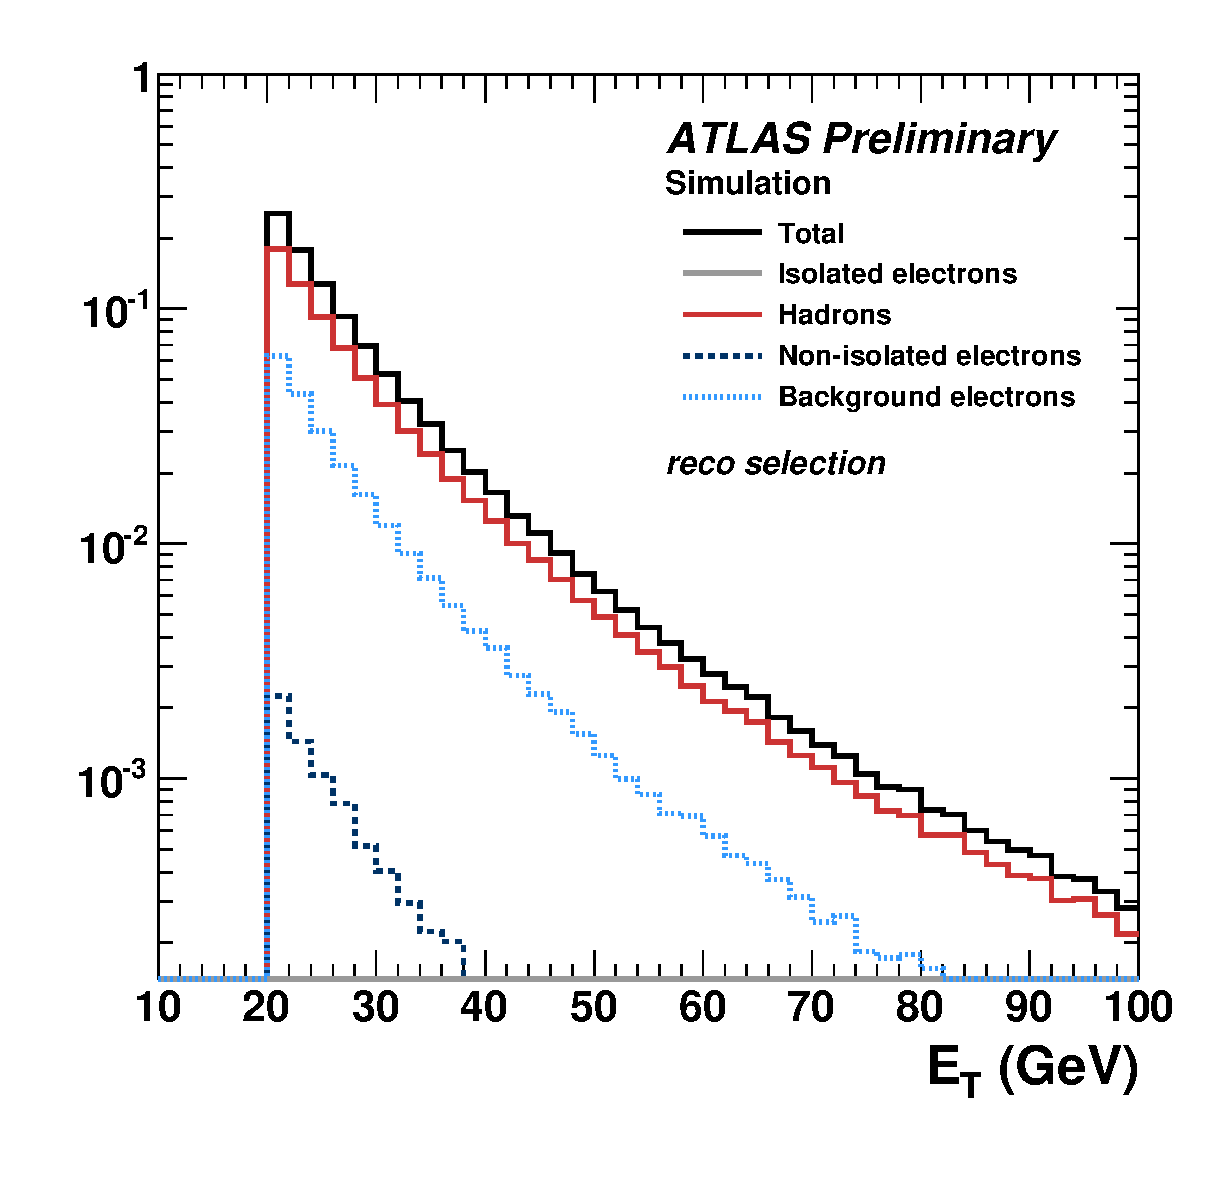
\includegraphics[width=\smallfigwidth]{tex/selection/electron_composition}
	\caption{The composition of reconstructed electrons as a function of transverse 
	energy, simulated by a \pythia{6} sample of di-jet, heavy flavour, prompt photon, \PW 
	and \PZ processes \cite{ElectronPerf:Expect}. Non-isolated electrons are from heavy 
	flavour decay. Background electrons are from photon conversions. Isolated electrons 
	are prompt electrons from a \PW or \PZ boson, though appear below the y-axis range.}
	\label{fig:objects:el_composition}
\end{figure}

\begin{description}
\item[Reconstruction] \hfill \\
	Energy deposits in \ac{ECal} cells are clustered by a \textit{sliding window} 
	algorithm \cite{ElectronPerf:Expect}. First, the calorimeter is divided into 
	\textit{towers} of size $\Delta\eta \times \Delta\phi = 0.025 \times 0.025$ (the 
	cell size of the middle layer). Then a window of $3 \times 5$ towers in $\eta$-$\phi$ 
	space scans the \ac{ECal} for local maxima with $E_T > \unit{2.5}{\GeV}$.

	Tracks within $\Delta R < 0.3$ of a cluster are then refit using a Gaussian Sum 
	Filter (GSF) \cite{Electron:GSF}. The default fit described in 
	\Section~\ref{sec:objects:tracks} uses a pion hypothesis to estimate material 
	effects, and does not account for the significant bremsstrahlung experienced by 
	electrons (which is highly $\eta$-dependent). The GSF is a non-linear fitter and 
	improves the accuracy of electron tracking by accounting for this.

	For a cluster to be reconstructed as an electron, it must be matched to a track. If a 
	track is within $\Delta\eta < 0.05$ and $\Delta\phi < 0.1 (0.05)$ of the cluster 
	centre, they are considered matched. The asymmetric $\Delta\phi$ requirement allows 
	for increased bending due to bremsstrahlung. When multiple tracks are matched, that 
	with the smallest $\Delta R$ is chosen.

	Finally, the cluster is rebuilt using a $3 \times 7$ ($5 \times 5$) sliding window 
	in the barrel (end-cap), and the electron four-momentum is defined 
	\cite{ElectronPerf:2010}. The direction is taken from the matched track and the 
	energy is the cluster energy, corrected for losses in passive material and leakage 
	outside the cluster. These simulated corrections depend on the longitudinal shower 
	shape and energy deposited in the presampler. The EM energy scale was calibrated
	using test beam and \textit{in situ} \HepProcess{\PZ \HepTo \Pe\Pe} measurements.
\item[Identification] \hfill \\
	Electron identification is improved by applying cuts on track quality and shower 
	shape. There are three reference operating points called \textit{loose}, 
	\textit{medium} and \textit{tight}, with progressively greater background rejection 
	and lower signal efficiency.
	
	For $E_T > \unit{25}{\GeV}$ the medium criteria are used, comprising cuts on
	\begin{itemize}[noitemsep,nolistsep]
		\item shower shape variables (lateral and longitudinal)
		\item leakage to the \ac{HCal}
		\item the number of pixel and \acs{SCT} hits
		\item the impact parameter with respect to the primary vertex
		\item track-cluster matching
		\item transition radiation
	\end{itemize}
	and additionally electrons with conversion vertices or without a hit in the first 
	pixel layer are vetoed (to suppress the \Wgamma background).
 
 	For $E_T < \unit{25}{\GeV}$ the \Wjets and QCD backgrounds are much larger. Thus a 
 	multivariate \textit{very tight likelihood} identification is used, with similar 
 	signal efficiency to the cut-based tight criteria but improved background rejection. 
 	It uses the signal and background probability density functions of multiple input 
 	variables to construct a likelihood discriminant, which may be cut upon (effectively 
 	choosing an operating point). The input variables are similar to those listed above, 
 	although track hits remain as cuts.
\item[Isolation] \hfill \\
	Rejection of hadronic fakes or electrons from heavy flavour decays is improved by 
	requiring the electron to be isolated from activity in the tracker and calorimeter. 
	The cuts are summarised in \Table~\ref{tab:objects:el_iso} and explained below.

	\textit{Tracker isolation:} $p_T^{\text{cone}}\parenths{R_0}$ is the summed $p_T$ of 
	all tracks of $p_T > \unit{0.4}{\GeV}$ within a cone of $\Delta R = R_0$, excluding 
	the electron track itself. For robustness against pile-up, the tracks are required to 
	originate from the primary vertex.

	\textit{Calorimeter isolation:} Uncalibrated topological clusters (see 
	\Section~\ref{sec:objects:jets}) are built from energy deposits in the \ac{ECal} 
	and \ac{HCal}. These are more robust against pile-up than cell deposits as they 
	suppress noise. $E_T^{\text{cone}}\parenths{R_0}$ is the summed $E_T$ of the 
	topological clusters within a cone of $\Delta R = R_0$, excluding cells in a 
	$5 \times 7$ window around the electron (see \Figure~\ref{fig:objects:el_iso}). 
	Corrections are made for electron energy leakage and deposits from pile-up and the 
	underlying event.
\item[Primary vertex association] \hfill \\
	To associate the electron with the primary vertex, the transverse impact parameter 
	$d_0$ is required to be within three standard deviations of zero. Also, the 
	longitudinal impact parameter $z_0$ is constrained by $\mods{z_0 \sin\theta} < 
	\unit{0.4}{\milli\metre}$.
\item[Efficiency] \hfill \\
	The efficiency of each selection step (reconstruction, identification, isolation and 
	primary vertex association) is measured via \textit{tag-and-probe} of 
	\HepProcess{\PZ \HepTo \Pe\Pe} events \cite{ElectronPerf:2010,ElectronPerf:2012}. 
	This involves selecting an unbiased sample of events containing a well-identified 
	\textit{tag} object and a loosely-identified \textit{probe} object, and measuring the 
	selection efficiency of the probes. The sample must be clean (often enforced by a 
	mass constraint) and backgrounds estimated (usually a side-bands or template fit).

	The tag is a well-identified electron, the probe is an electron passing the previous 
	step (or an \ac{ECal} cluster) and the constraint is $\unit{80}{\GeV} < 
	m_{\parenths{\text{tag, probe}}} < \unit{100}{\GeV}$. The reconstruction and 
	identification efficiencies are shown in \Figure~\ref{fig:objects:el_recoeff} and 
	\Figure~\ref{fig:objects:el_ideff} respectively. Comparison with MC yields efficiency 
	scale factors.
\end{description}

\begin{figure}
	\includegraphics[width=0.495\textwidth]{tex/selection/el_recoeff_et}
	\hfill
	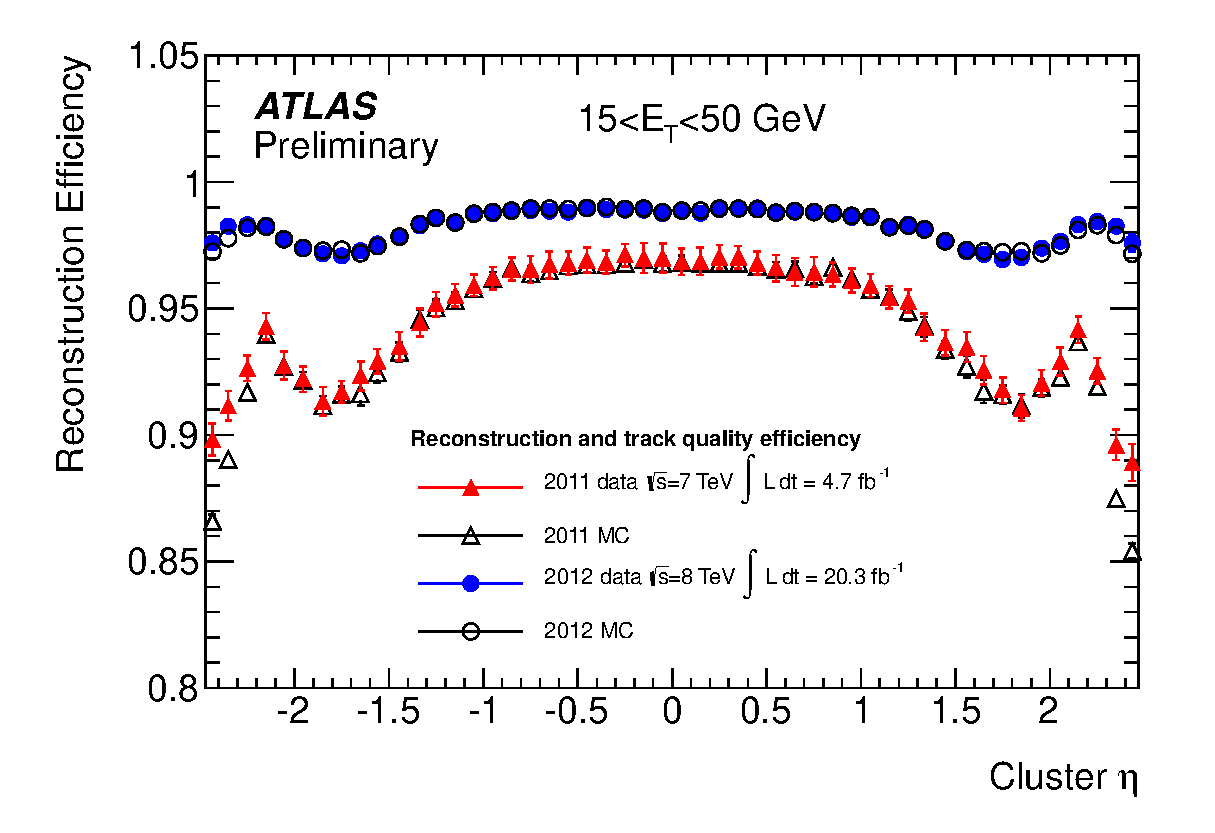
\includegraphics[width=0.495\textwidth]{tex/selection/el_recoeff_eta}
	\caption{The electron reconstruction efficiency versus (left) $E_T$ and (right) 
	$\eta$, measured using tag-and-probe of \HepProcess{\PZ \HepTo \Pe\Pe} data 
	and compared to MC \cite{ElectronPerf:2012}. In 2012, the implementation of GSF 
	tracking gave significant performance improvement.}
	\label{fig:objects:el_recoeff}
\end{figure}

\begin{figure}
	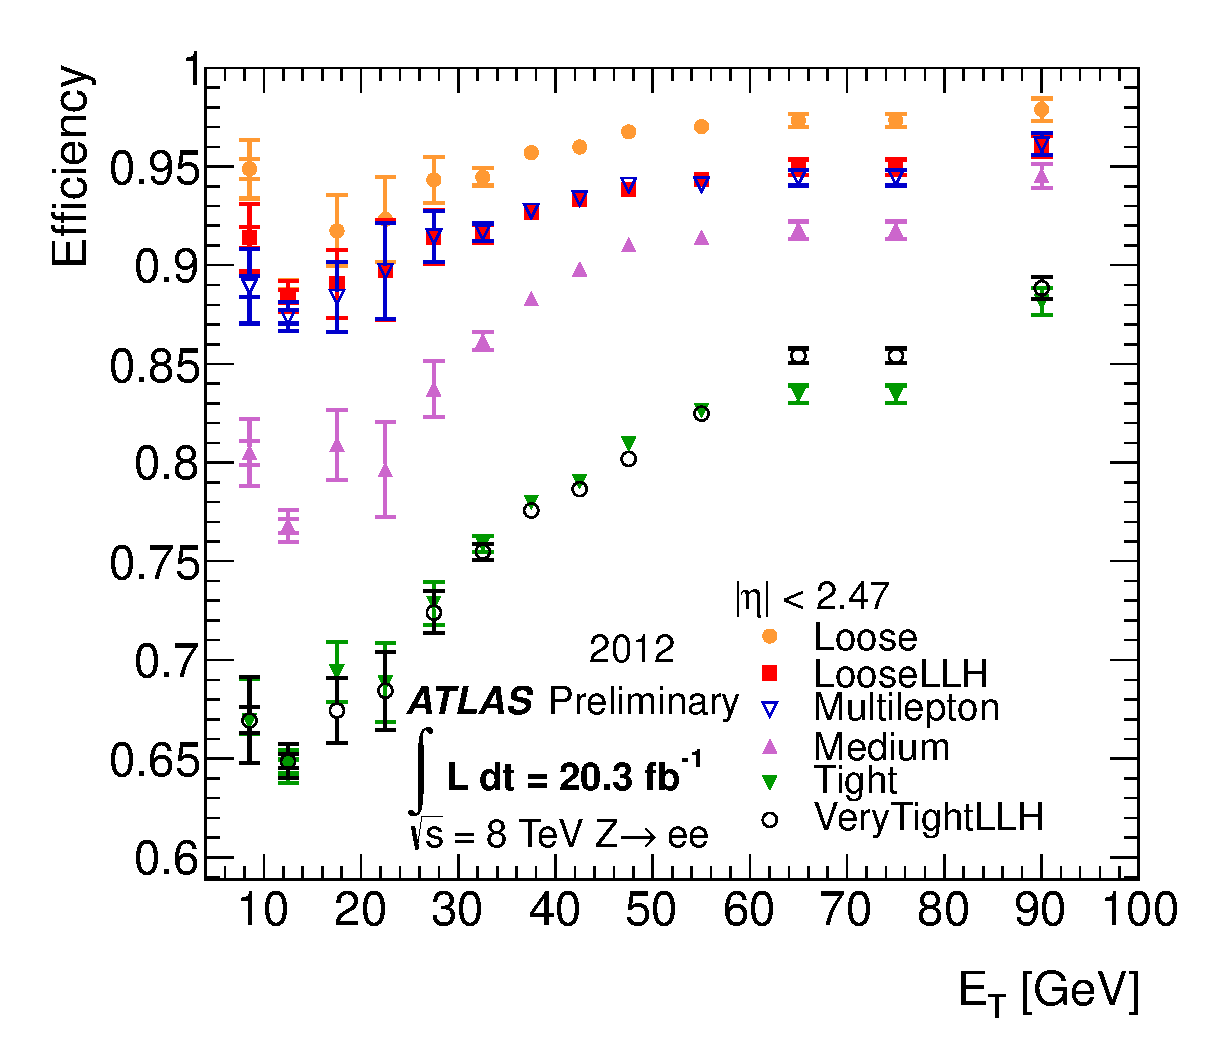
\includegraphics[width=0.495\textwidth]{tex/selection/el_ideff_et}
	\hfill
	\includegraphics[width=0.495\textwidth]{tex/selection/el_ideff_npv}
	\caption{The efficiency of a variety of electron identification operating points 
	versus (left) $E_T$ and (right) \npv, measured using tag-and-probe of 
	\HepProcess{\PZ \HepTo \Pe\Pe} data \cite{ElectronPerf:2012}. `Very tight likelihood' 
	has similar efficiency to `tight', but improves background rejection. All operating 
	points are fairly robust against pile-up.}
	\label{fig:objects:el_ideff}
\end{figure}

\begin{table}[h]
	\begin{tabular}{c@{\hskip 0.3in}c@{\hskip 0.3in}c}
		Electron $E_T$ (\GeV) & Tracker isolation & Calorimeter isolation \\
		\hline
		10 -- 15 & $p_T^{\text{cone}}\parenths{0.4}/E_T < 0.06$ & $E_T^{\text{cone}}\parenths{0.3}/E_T < 0.20$ \\
		15 -- 20 & $p_T^{\text{cone}}\parenths{0.3}/E_T < 0.08$ & $E_T^{\text{cone}}\parenths{0.3}/E_T < 0.24$ \\
		$> 20$   & $p_T^{\text{cone}}\parenths{0.3}/E_T < 0.10$ & $E_T^{\text{cone}}\parenths{0.3}/E_T < 0.28$ \\
	\end{tabular}
	\caption{The tracker and calorimeter isolation requirements of electrons. The cuts 
	were chosen to optimise the sensitivity of a low mass \HWWlvlv search.}
	\label{tab:objects:el_iso}
\end{table}

\begin{figure}
	\includegraphics[width=\smallfigwidth]{tex/selection/el_isolation}
	\caption{Schematic diagram to illustrate calorimeter isolation. The pink cells are 
	topological clusters, the yellow circle is the isolation cone ($R_0 = 0.4$ shown), 
	the green $3 \times 7$ rectangle is the reconstructed electron cluster, and the white 
	$5 \times 7$ rectangle is the area removed from the cone.}
	\label{fig:objects:el_iso}
\end{figure}



\subsection{Muons}
\label{sec:objects:muons}

A muon will pass through the \ac{ID}, deposit minimal energy in the calorimeters and 
continue through the \ac{MS}. Thus, they can be found via activity in the \ac{MS}, 
optionally matched to an \ac{ID} track. Muons with $p_T > \unit{10}{\GeV}$ and 
$\mods{\eta} < 2.5$ are selected.

\begin{description}
\item[Reconstruction] \hfill \\
	Muons are found by matching \ac{MS} tracks to \ac{ID} tracks\footnote{
		A variety of muon reconstruction strategies are available: \textit{stand-alone} 
		muons have only \ac{MS} tracks, \textit{combined} muons have both \ac{MS} and 
		\ac{ID} tracks, \textit{segment-tagged} muons have \ac{ID} tracks that match to 
		\iac{MS} track segment, and \textit{calorimeter-tagged} muons have \ac{ID} 
		tracks matched to the calorimeter deposit of a minimum ionising particle (used to 
		recover efficiency at $\eta \approx 0$, where detector services reduce the \ac{MS}
		coverage). This thesis uses \textit{combined} muons, which perform best.
	}
	and their momenta are measured from track curvature \cite{ATLAS:ExpectPerf}.

	First, the \textit{Muonboy} algorithm \cite{Muons:algorithms} identifies a 
	$\Delta\eta \times \Delta\phi \approx 0.4 \times 0.4$ region of activity via the muon 
	trigger chambers (see \Section~\ref{sec:atlas:ms}) and then reconstructs localised 
	segments from nearby \acs{MDT} and \acs{CSC} hits. By scanning a potential momentum 
	range, segments in different layers are combined to form a track. Finally, a global 
	track fit using the full \ac{MS} hit information is performed, accounting for energy 
	loss.

	\ac{MS} tracks are extrapolated to the primary vertex, accounting for energy loss in 
	the calorimeter, and matched to \ac{ID} tracks (see 
	\Section~\ref{sec:objects:tracks}). The statistical combination of the two 
	tracks is performed by the \textit{STACO} algorithm \cite{Muons:algorithms}, which
	weights each track by its covariance matrix. The muon four-momentum is determined 
	by this combined track (dominated by the \ac{ID} track at low-$p_T$ and by the 
	\ac{MS} track at high-$p_T$), and is calibrated with \HepProcess{\PZ \HepTo \Pmu\Pmu}
	events \cite{Muons:2012}.
\item[Isolation] \hfill \\
	Although the muon signature is much cleaner than that of electrons, hadronic fakes 
	(\textit{punch-through}) and muons from heavy flavour decays must still be suppressed 
	by isolation criteria, which are summarised in \Table~\ref{tab:objects:mu_iso}. The 
	$p_T^{\text{cone}}\parenths{R_0}$ and $E_T^{\text{cone}}\parenths{R_0}$ variables are 
	defined similarly to electrons, though the size of the subtracted calorimeter window 
	is reduced for muons.
\item[\ac{ID} track quality] \hfill \\
	The \ac{ID} track must satisfy quality criteria on the number of traversed sensors:
	\begin{itemize}[noitemsep,nolistsep]
		\item $n_{\text{pixel}}^{\text{hit}} + n_{\text{pixel}}^{\text{dead}} > 0$
		\item $n_{\text{SCT}}^{\text{hit}} + n_{\text{SCT}}^{\text{dead}} > 4$
		\item $n_{\text{pixel}}^{\text{hole}} + n_{\text{SCT}}^{\text{hole}} < 3$
		\item $n_{\text{TRT}}^{\text{hit}} + n_{\text{TRT}}^{\text{outlier}} > 5$ and at 
		least 10\% are hits (for $\mods{\eta} < 1.9$ only)
	\end{itemize}
	where a hole is an expected hit that is not observed.
\item[Primary vertex association] \hfill \\
	To associate the muon with the primary vertex, the transverse impact parameter $d_0$ 
	is required to be within three standard deviations of zero. Also, the longitudinal 
	impact parameter $z_0$ is constrained by $\mods{z_0 \sin\theta} < 
	\unit{1.0}{\milli\metre}$.
\item[Efficiency] \hfill \\
	The efficiency of each selection step is measured via \textit{tag-and-probe} of 
	\HepProcess{\PZ \HepTo \Pmu\Pmu} events \cite{Muons:2012}. For example, the 
	reconstruction efficiency is shown in \Figure~\ref{fig:objects:mu_recoeff}. 
	Comparison with MC yields efficiency scale factors.
\end{description}

\begin{table}[h]
	\begin{tabular}{c@{\hskip 0.3in}c@{\hskip 0.3in}c}
		Muon $p_T$ (\GeV) & Tracker isolation & Calorimeter isolation \\
		\hline
		10 -- 15 & $p_T^{\text{cone}}\parenths{0.4}/p_T < 0.06$ & $E_T^{\text{cone}}\parenths{0.3}/p_T < 0.06$ \\
		15 -- 20 & $p_T^{\text{cone}}\parenths{0.3}/p_T < 0.08$ & $E_T^{\text{cone}}\parenths{0.3}/p_T < 0.12$ \\
		20 -- 25 & $p_T^{\text{cone}}\parenths{0.3}/p_T < 0.12$ & $E_T^{\text{cone}}\parenths{0.3}/p_T < 0.18$ \\
		$> 25$   & $p_T^{\text{cone}}\parenths{0.3}/p_T < 0.12$ & $E_T^{\text{cone}}\parenths{0.3}/p_T < 0.30$ \\
	\end{tabular}
	\caption{The tracker and calorimeter isolation requirements of muons. The cuts were 
	chosen to optimise the sensitivity of a low mass \HWWlvlv search.}
	\label{tab:objects:mu_iso}
\end{table}

\begin{figure}
	\includegraphics[width=0.495\textwidth]{tex/selection/mu_recoeff_pt}
	\hfill
	\includegraphics[width=0.495\textwidth]{tex/selection/mu_recoeff_eta}
	\caption{The muon reconstruction efficiency versus (left) $p_T$ and (right) 
	$\eta$, measured using tag-and-probe of \HepProcess{\PZ \HepTo \Pmu\Pmu} data 
	and compared to MC \cite{Muons:2012}. Reductions in efficiency at $\eta \approx 0$ 
	and $\eta \approx 1.2$ are due to partial \ac{MS} coverage (detector services and 
	incomplete installation respectively). `Chain 1' refers to \textit{STACO} 
	reconstruction.}
	\label{fig:objects:mu_recoeff}
\end{figure}



\subsection{Jets}
\label{sec:objects:jets}

A hadron will pass through the \ac{ID} (leaving hits if charged) before being absorbed by 
the \ac{ECal} and \ac{HCal}. Due to the finite resolution of the calorimeter and the 
large number of overlapping hadronic showers, it is impossible to reconstruct individual 
hadrons. For this and more theoretical reasons outlined in \Section~\ref{sec:jets}, 
energy deposits are used to reconstruct jets. The main challenge in identifying jets from 
the hard scatter is calorimeter noise: both electronic and from pile-up.

Jets are selected with $p_T > \unit{25}{\GeV}$ for central jets ($\mods{\eta} < 2.4$) and 
with $p_T > \unit{30}{\GeV}$ for forward jets ($2.4 < \mods{\eta} < 4.5$). However, 
occasionally it is useful to use jets with other $p_T$ thresholds (\eg the central jet 
veto in the VBF search). It shall be clearly stated when this is the case.

\begin{description}
\item[Reconstruction] \hfill \\
	To suppress contributions from calorimeter noise, energy deposits are grouped into 
	topological clusters (\textit{topo-clusters}) \cite{Jets:Calib:2010,Jets:Calib:2011}. 
	First, a seed cell is identified with signal-to-noise ratio $S/N > 4$. Surrounding 
	cells with $S/N > 2$ are iteratively added. Finally, a single iteration of 
	neighbouring cells with no $S/N$ cut are added. When localised maxima exist within a 
	cluster, it may be split. Clearly, the robustness to noise is determined by $N$, 
	which is taken to be the sum in quadrature of the electronic noise and the pile-up 
	noise expected with $\mu = 30$.

	The non-compensating calorimeter design gives differing responses to electromagnetic 
	and hadronic showers.\footnote{
		Significant hadronic shower energy is lost through slow neutrons, nuclear 
		excitations and neutrinos.
	}
	Topo-clusters are reconstructed at the EM scale and thus need calibration to the 
	\ac{JES}. An intermediate \textit{local cluster weighting} (LCW) classifies 
	topo-clusters as electromagnetic or hadronic (via energy density and shower depth) 
	and applies appropriate energy corrections.
	
	These topo-clusters are input to the \antikt jet algorithm with $R = 0.4$ (see 
	\Section~\ref{sec:jets}), making the assumption that topo-clusters are massless.
\item[Calibration] \hfill \\
	There are four steps to the jet calibration, described below \cite{Jets:Calib:2011}.

	First, the jet direction is adjusted such that it originates from the primary vertex, 
	rather than the centre of the ATLAS coordinate system.

	Second, energy contributed by pile-up is subtracted \cite{Jets:PileupCorrection:2012}.
	This involves measuring the jet area $A$ (its susceptibility to additional soft 
	particles) and the pile-up density $\rho$ of the event. Residual corrections for 
	in-time pile-up (via \npv) and out-of-time pile-up (via $\mu$) are also made. Thus,
	the correction is
	\begin{equation}
		p_T^{\text{corr}} = p_T - \rho A - \alpha \parenths{\npv - 1} - \beta \mu
	\end{equation}
	and its impact upon the robustness against pile-up is shown in 
	\Figure~\ref{fig:objects:jet_pu_corr}.

	Third, the energy is calibrated from the LCW scale to the \ac{JES}. The correction is 
	derived from MC by comparing the energy of the reconstructed jet to that of the 
	corresponding hadron-level jet (\ie before detector simulation).

	Finally, a residual \textit{in situ} \ac{JES} calibration corrects for mismodelling, 
	and is applied to jets in data events only. The calibration exploits the $p_T$ 
	balance between a jet and a well-measured reference object, deriving the correction 
	as the double-ratio
	\begin{equation}
		\angles{p_T^{\text{jet}} / p_T^{\text{ref}}}_{\text{\!MC}} \,\, \Big/ 
		\angles{p_T^{\text{jet}} / p_T^{\text{ref}}}_{\text{\!data}} \,\,.
	\end{equation}
	The reference object is chosen to be a \PZ boson (decaying to \epluseminus or 
	\HepProcess{\APmuon\Pmuon}) at low $p_T$, a photon at medium $p_T$, or a system of 
	well-calibrated low-$p_T$ jets at high $p_T$. The contribution of each technique to 
	the correction is shown in \Figure~\ref{fig:objects:jet_insitu}.
\item[Quality] \hfill \\
	`Looser' quality to reject calo noise faking jets by looking at cell pulse shapes (ATLAS-CONF-2012-020)
\item[Primary vertex association] \hfill \\
	JVF > 0.5 (central jets with $p_T < \unit{50}{\GeV}$ only)
	effective pile-up suppression
	efficiency SF
\end{description}

\begin{figure}
	\includegraphics[width=0.495\textwidth]{tex/selection/jet_pu_npv}
	\hfill
	\includegraphics[width=0.495\textwidth]{tex/selection/jet_pu_mu}
	\caption{The dependence of jet $p_T$ on (left) in-time pile-up and (right) 
	out-of-time pile-up, versus $\mods{\eta}$ \cite{Jets:PileupCorrection:2012}. The 
	bands show the fits used in the correction.}
	\label{fig:objects:jet_pu_corr}
\end{figure}

\begin{figure}
	\includegraphics[width=\mediumfigwidth]{tex/selection/jet_insitu_corr}
	\caption{The ratio of the jet response measured in data to the MC prediction versus 
	jet $p_T$. This is the inverse of the \textit{in situ} JES correction (see text). The 
	results of three $p_T$ balance studies and their combination (black line) are shown.}
	\label{fig:objects:jet_insitu}
\end{figure}



\subsection{\Pbottom-jets}
\label{sec:objects:bjets}

suppress top background

MV1 85\% operating point
efficiency from dileptonic ttbar events with combined likelihood method (not tag-and-probe)
b-tagging efficiency SF


\subsection{Missing transverse momentum}
\label{sec:objects:met}

hermetic design => incoming partons have very little transverse momentum => momentum conservation used to infer vector sum transverse momentum of non-interacting particles
True MET (neutrinos), Fake MET (mismeasurement, noise, etc)

\subsubsection{Track-based \met}

\subsubsection{Calorimeter-based \met}

    \section{Event selection criteria}
      \label{sec:selection}
      %!TEX root = ../../thesis.tex

\Section~\ref{sec:signature} outlined the basic experimental signature of the search as 
two oppositely charged leptons and significant \met. Thus, the initial stages of the 
event selection are responsible for finding this signature. Subsequent criteria, or 
\textit{cuts}, target specific background processes. Their aim is to improve the analysis 
sensitivity by suppressing backgrounds whilst retaining a sufficient number of signal events.



\subsection{Data quality}
\label{sec:selection:quality}

The \pp dataset (see \Section~\ref{sec:dataset:dataset}) is hierarchically split into 
\textit{periods} of broadly consistent beam conditions, \textit{runs} typically 
corresponding to LHC fills, and \textit{luminosity blocks} of \about 2~minutes where the 
instantaneous luminosity is approximately constant. Luminosity blocks are included in the 
analysis if the detector was operating sufficiently for the recorded data to be 
considered `good for physics' (see \Figure~\ref{fig:dataset:lumi}).\footnote{
	ATLAS good runs list: \texttt{data12\symbol{95}8TeV.periodAllYear\symbol{95}DetStatus-v61-pro14-02\symbol{95}DQDefects-00-01
	-00\symbol{95}PHYS\symbol{95}StandardGRL\symbol{95}All\symbol{95}Good.xml}
} 
For the 2012 dataset, this corresponds to a total integrated luminosity of 
\unit{20.3}{\invfb}.

Individual events are also vetoed if certain data quality criteria are failed by:
\begin{itemize}[noitemsep,nolistsep]
	\item a noise burst in the LAr calorimeter,
	\item data corruption caused by a restart of the synchronisation system,
	\item a \textit{looser} jet is reconstructed with \unit{$\pt > 20$}{\GeV} (indicative 
	of an HCal spike),
	\item a jet is reconstructed near a `hot' HCal tile (1st -- 8th May 2012 only).
\end{itemize}
A further quality criterion requires that the primary vertex considered as the hard 
scatter (that with the highest $\sum p_{\text{T}}^2$) must be associated with at least 
three tracks. This reduces the cosmic ray background to negligible levels.



\subsection{Trigger}
\label{sec:selection:trigger}

It is infeasible to record all the delivered collisions; ATLAS employs a trigger system to 
identify and record interesting events (see \Section~\ref{sec:atlas:trig}). In the \HWWlvlv 
search it is natural to trigger on high-\pt leptons, using algorithms similar to, though less 
sophisticated than, those in \Section~\ref{sec:objects:electrons} and 
\Section~\ref{sec:objects:muons}.

A trigger is characterised by its efficiency versus \pt curve (though it also depends on 
$\eta$), which has a turn-on followed by a plateau, as shown in 
\Figure~\ref{fig:sel:trig_eff}. It is preferable to operate on the plateau, where the 
efficiency is more stable and has smaller uncertainty. To maximise the signal yield, it is 
desirable to use a trigger with a lower turn-on \pt. However, increased backgrounds and 
limitations to trigger latency and bandwidth require a compromise to be found. The lowest 
unprescaled\footnote{
	A \textit{prescaled} trigger reduces the turn-on \pt by recording only 1 in $N$ 
	events passing the trigger, and weighting such events by a factor $N$. In doing so, 
	some statistical power is lost.
}
single lepton triggers available in 2012 had nominal \pt thresholds of \unit{24}{\GeV}. 
Fortunately, it is possible to recover trigger efficiency at lower \pt by using dilepton 
triggers, because the backgrounds are much smaller.

\begin{figure}[t]
	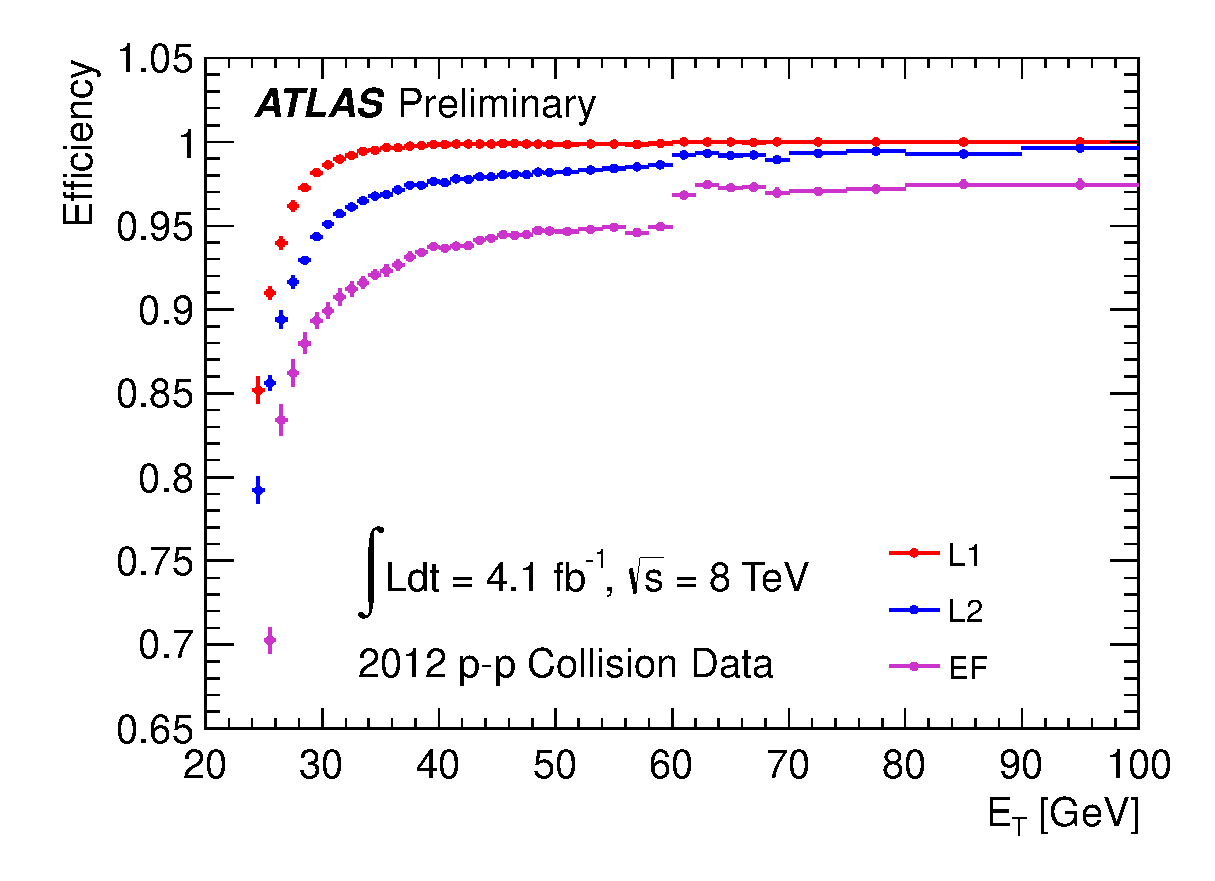
\includegraphics[width=0.495\textwidth]{tex/selection/trigger_eff_el}
	\hfill
	\includegraphics[width=0.495\textwidth]{tex/selection/trigger_eff_mu}
	\caption{Efficiencies of the single lepton triggers for electrons with respect to 
	offline \textit{medium} identification (left) and muons with respect to offline 
	reconstruction (right).}
	\label{fig:sel:trig_eff}
\end{figure}

\begin{table}[t]
	\begin{tabular}{lllcl}
		\toprule
		\multirow{2}{2.5cm}{Single lepton triggers} & \Pe  & \verb|EF_e24vhi_medium1| & or & \verb|EF_e60_medium1| \\
		& \Pmu & \verb|EF_mu24i_tight| & or & \verb|EF_mu36_tight|  \\
		\midrule
		\multirow{3}{2.5cm}{Dilepton triggers} & \HepProcess{\Pe\Pe} & \verb|EF_2e12Tvh_loose1| & or & \verb|EF_2e12Tvh_loose1_L2StarB| \\
		& \HepProcess{\Pmu\Pmu} & \multicolumn{3}{l}{\texttt{EF\symbol{95}mu18\symbol{95}tight\symbol{95}mu8\symbol{95}EFFS}} \\
		& \HepProcess{\Pe\Pmu}  & \multicolumn{3}{l}{\texttt{EF\symbol{95}e12Tvh\symbol{95}medium1\symbol{95}mu8}} \\
		\bottomrule
	\end{tabular}
	\caption{Employed triggers. \texttt{EF} refers to event filter, \texttt{e} is an 
	electron, \texttt{mu} is a muon, the following number is the \pt threshold, 
	\texttt{vh} indicates calorimeter isolation, \texttt{i} indicates track isolation, 
	and \texttt{tight}, \texttt{medium} or \texttt{loose} is the identification. Other 
	parts relate to the trigger chain. Criteria are looser than those applied 
	offline.}
	\label{tab:sel:triggers}
\end{table}

Events are required to pass at least one trigger listed in \Table~\ref{tab:sel:triggers}. 
The single lepton triggers include a tighter low-\pt trigger and a looser high-\pt 
trigger in order to maximise the efficiency. Dilepton triggers are then used to recover some 
efficiency at lower \pt. Together, these triggers support a \pt threshold of \unit{22}{\GeV} 
on the leading lepton (in the offline analysis), whilst operating on the plateau.

Additionally, events are required to have at least one lepton passing the offline 
reconstruction that is matched within $\Delta R < 0.15$ of a triggered lepton object.
Single lepton triggers are matched to offline leptons with $\pt > \unit{25}{\GeV}$. On 
the other hand, dilepton triggers comprise two triggered objects: \texttt{mu8} is matched 
to offline muons with $\pt > \unit{10}{\GeV}$, \texttt{mu18} is matched to offline muons 
with $\pt > \unit{20}{\GeV}$, and \texttt{e12} is matched to offline electrons with 
$\pt > \unit{15}{\GeV}$.\footnote{
	It follows that events featuring an electron with \unit{$\pt < 15$}{\GeV} must fire a 
	single lepton trigger, and thus the leading lepton must have \unit{$\pt > 25$}{\GeV}.
}

Lepton trigger efficiencies are measured via tag-and-probe of 
\HepProcess{\PZ \HepTo \Plepton\Plepton} events, where the tag and probe have both 
passed the offline lepton selection and the tag has successfully matched to a triggered 
lepton object. For example, single lepton trigger efficiencies are displayed in 
\Figure~\ref{fig:sel:trig_eff}. Comparison with MC yields efficiency scale factors.



\subsection{Pre-selection of dilepton + \met signature}
\label{sec:selection:presel}

Following the trigger selection, events are required to have two oppositely charged 
leptons passing the offline selection (see \Section~\ref{sec:objects}). The lepton with 
the highest \pt, called the \textit{leading lepton}, must have 
\unit{$\ptleadlep > 22$}{\GeV} in order to operate on the trigger plateau. The 
\textit{subleading lepton} must have \unit{$\ptsubleadlep > 10$}{\GeV}, as specified in 
\Section~\ref{sec:objects}. Events containing a third lepton are vetoed in order to 
reject backgrounds with three or more leptons in the final state, such as \WZ production.

At this point, it is possible to split the dilepton final state into four channels 
according to the flavours of the two leptons: \eech, \mmch, \emch, \mech (where the first 
flavour is that of the leading lepton). This is very useful because the background 
compositions of the channels are dramatically different. For example, the \DYll background 
is much larger in the same flavour channels (\eech/\mmch) than the different flavour 
channels (\emch/\mech).

Low mass hadronic resonances with dileptonic decays (\eg \PJpsi) are removed from the 
\eech/\mmch channels by requiring the mass of the dilepton system \unit{$\mll > 12$}{\GeV}. 
This also greatly suppresses the low mass \DY background. For the \emch/\mech channels, 
a cut of \unit{$\mll > 10$}{\GeV} suppresses leptons from heavy flavour decays. The 
\eech/\mmch channels are hugely dominated by the \DY background (see 
\Figure~\ref{fig:sel:mll}), but most of these events can be rejected by 
vetoing a window around the \PZ mass, \unit{$\mods{\mll - \mZ} > 15$}{\GeV}.

\begin{figure}
	\includegraphics[width=0.495\textwidth]{tex/selection/emme_CutMll_Mll_mh125_log}
	\hfill
	\includegraphics[width=0.495\textwidth]{tex/selection/eemm_CutMll_Mll_mh125_log}
	\caption{The \mll distribution in the \emch/\mech (left) and \eech/\mmch (right) 
	channels. These are made after the low \mll cut.}
	\label{fig:sel:mll}
\end{figure}

\begin{figure}
	\includegraphics[width=0.495\textwidth]{tex/selection/emme_CutZVeto_MET_TrackHWW_Clj_mh125_log}
	\hfill
	\includegraphics[width=0.495\textwidth]{tex/selection/eemm_CutZVeto_METRel_mh125_log}
	\caption{The \met variable cut upon in the \emch/\mech (left) and \eech/\mmch (right) 
	channels. These are made after the \PZ mass veto cut.}
	\label{fig:sel:met}
\end{figure}

Requiring significant \met suppresses the \DYll and dijet backgrounds (see 
\Figure~\ref{fig:sel:met}). It also suppresses the \DYtt background as its neutrinos have a 
propensity to cancel in the \met calculation. We require \unit{$\corrtrackmet > 20$}{\GeV} 
in the \emch/\mech channels and \unit{$\metrel > 40$}{\GeV} in the \eech/\mmch channels. In 
the \emch/\mech channels, the \met cut is relaxed because the \DYll background is smaller. 

Following the selection of dilepton events with significant \met, the \emch/\mech 
channels are dominated by top background and the \eech/\mmch channels are dominated by 
\DYll. However, the background compositions of all channels are highly dependent upon the 
number of jets (see \Figure~\ref{fig:sel:njets}). Thus, at this stage the analysis is 
binned according to jet multiplicity (0-jet, 1-jet, \twojet), so that backgrounds can be 
targeted individually. In the \twojet bin, only the \emch/\mech channels are used.

\begin{figure}[t]
	\includegraphics[width=0.495\textwidth]{tex/selection/emme_CutMETRel_m_jet_n_upTo7_mh125_lin}
	\hfill
	\includegraphics[width=0.495\textwidth]{tex/selection/eemm_CutMETRel_m_jet_n_upTo7_mh125_lin}
	\caption{Jet multiplicity distribution in the \emch/\mech (left) and \eech/\mmch (right) 
	channels. These are made following the pre-selection.}
	\label{fig:sel:njets}
\end{figure}



\subsection{\HWWlvlv decay topology}
\label{sec:selection:higgs_decay}

The discrimination of \HWW signal from irreducible backgrounds that also feature a \WW pair 
is a problem common to all jet bins. Thus, the topology of the \HWWlvlv decay is discussed 
before continuing with the event selection.

Firstly, the spin-0 nature of the Higgs boson and the \VminusA structure of the weak 
interaction (see \Section~\ref{sec:ewsb}) imply that a small opening angle between the 
two leptons is preferred. This follows from spin conservation and the extremely small 
masses of the neutrinos. Consequently, the mass of the dilepton system, \mll, is also 
small. This follows from $m_{\Plepton\Plepton}^2 \simeq m_{\Plepton_1}^2 + 
m_{\Plepton_2}^2 + 2 E_{\Plepton_1} E_{\Plepton_2} \parenths{1 - \cos\vartheta}$, where 
$\vartheta$ is the opening angle. Thus, signal events are selected with the criteria 
$\dphill < 1.8$ and \unit{$\mll < 55$}{\GeV}.

Secondly, the invariant mass of the dilepton + dineutrino system should correspond to 
\mH (modified by a Breit-Wigner distribution). Unfortunately, as discussed above, it is 
only possible to infer the \textit{transverse} component of the dineutrino system 
momentum. We therefore construct a transverse mass variable
\begin{equation}
	\mt = \sqrt{\parenths{\etll + \corrtrackmet}^2 - \mods{\ptllvec + \corrtrackmetvec}^2}
\end{equation}
where $E_{\text{T,\HepProcess{\Plepton\Plepton}}}^2 = 
p_{\text{T,\HepProcess{\Plepton\Plepton}}}^2 + m_{\Plepton\Plepton}^2$ and 
\corrtrackmetvec 
is used as it has the best resolution (see \Section~\ref{sec:objects:met}). At 
hadron-level this is an event-by-event lower bound on \mH, though at detector-level the 
sharp cut-off is smeared by the poor \corrtrackmet resolution. This \mt observable is used in 
the statistical fitting procedure.



\subsection{0-jet selection}
\label{sec:selection:0j}

The 0-jet bin is dominated by \DY and \WW backgrounds. A small number of pathological 
events where \metvec is near \ptllvec are rejected by requiring $\dphillmet > \pi/2$.

Considering the \DYll background, the boson \pt will generally be less than the \pt 
threshold used in jet selection, since no jet has been found. Thus, the \DY background is 
greatly reduced by requiring \unit{$\ptll > 30$}{\GeV} (see 
\Figure~\ref{fig:sel:0j:ptll}). In the \eech/\mmch channels only, the \DYll background is 
also suppressed by an additional cut \unit{$\trackmetrel > 40$}{\GeV} (see 
\Figure~\ref{fig:sel:0j:sf_cuts}).

\begin{figure}[t]
	\includegraphics[width=0.495\textwidth]{tex/selection/emme_CutDPhillMET_0jet_Ptll_mh125_log}
	\hfill
	\includegraphics[width=0.495\textwidth]{tex/selection/eemm_CutDPhillMET_0jet_Ptll_mh125_log}
	\caption{The \ptll distribution in the \emch/\mech (left) and \eech/\mmch (right) 
	channels. These are made in the 0-jet bin, after the \dphillmet cut.}
	\label{fig:sel:0j:ptll}
\end{figure}

After the signal topology selection (see \Section~\ref{sec:selection:higgs_decay}), a 
large \DYll background remains in the \eech/\mmch channels, despite the significant \met 
requirements. This can be further suppressed by searching for soft hadronic activity to 
balance the dilepton system. First, jets with \unit{$\pt > 10$}{\GeV} and $\mods{\eta} < 
4.5$ are found (as detailed in \Section~\ref{sec:objects:jets}, minus the JVF cut). 
Then a discriminant is defined
\begin{equation}
	\frecoil = \left. \mods{\sum\limits_{j\text{ in }\wedge} \text{JVF}_{j} \cdot \bvec{p}_{\text{T,}j}} \, \middle/ \ptll \right.
	\label{eq:frecoil}
\end{equation}
where $\wedge$ is the detector quadrant centred on $-\ptllvec$. This is essentially the 
fraction of \ptll that can be balanced by soft hadronic activity in the opposing quadrant,
and so is larger in \DYll than processes with neutrinos. We require $\frecoil < 0.1$ in 
the \eech/\mmch channels (see \Figure~\ref{fig:sel:0j:sf_cuts}). \frecoil is also 
instrumental in estimating the \DYll background, and shall be revisited in 
\Section~\ref{sec:dy}.

\begin{figure}
	\includegraphics[width=0.495\textwidth]{tex/selection/eemm_CutTopoMll_0jet_METRel_TrackHWW_mh125_log}
	\hfill
	\includegraphics[width=0.495\textwidth]{tex/selection/eemm_CutTopoDPhill_0jet_f_recoil_mh125_log}
	\caption{The \trackmetrel (left) and \frecoil (right) distributions in the \eech/\mmch 
	channels, directly before they are cut upon.}
	\label{fig:sel:0j:sf_cuts}
\end{figure}

The event yields of the 0-jet selection are provided in \Appendix~\ref{app:sr_yields}, 
and the \mt distributions of the selected events are shown in \Figure~\ref{fig:sel:0j:mt}.

\begin{figure}
	\includegraphics[width=0.495\textwidth]{tex/selection/emme_CutFRecoil_0jet_MT_TrackHWW_Clj_mh125_lin}
	\hfill
	\includegraphics[width=0.495\textwidth]{tex/selection/eemm_CutFRecoil_0jet_MT_TrackHWW_Clj_mh125_lin}
	\caption{The \mt distribution of the selected 0-jet events, in the \emch/\mech (left) and 
	\eech/\mmch (right) channels.}
	\label{fig:sel:0j:mt}
\end{figure}



\subsection{1-jet selection}
\label{sec:selection:1j}

The 1-jet bin is initially dominated by the \DY and top backgrounds (see 
\Figure~\ref{fig:sel:njets}), though the top background is efficiently reduced by vetoing 
events containing a \Pbottom-tagged jet with \unit{$\pt > 20$}{\GeV} (see 
\Section~\ref{sec:objects:bjets}).

In order to reduce the dijet background, which has a large uncertainty, two single-lepton 
transverse mass variables are constructed
\begin{equation}
	m_{\text{T,}\Plepton_i} = \sqrt{2 \, p_{\text{T,}\Plepton_i} \, \corrtrackmet 
	\sqbracs{1 - \cos\Delta\phi\parenths{\Plepton_i, \corrtrackmet}}} \,.
\end{equation}
Their maximum, \maxmtw, tends to peak at lower values for processes with fake \met (see 
\Figure~\ref{fig:sel:1j:df_cuts}). Therefore we require \unit{$\maxmtw > 50$}{\GeV} in the 
\emch/\mech channels. In the \eech/\mmch channels, the tighter \met cuts reject the dijet 
background.

\begin{figure}[t]
	\includegraphics[width=0.495\textwidth]{tex/selection/emme_CutbVeto_1jet_MaxMTW_TrackHWW_Clj_mh125_lin}
	\hfill
	\includegraphics[width=0.495\textwidth]{tex/selection/emme_CutMaxMTlep_1jet_Mtt_TrackHWW_Clj_mh125_lin}
	\caption{The \maxmtw (left) and \mtautau (right) distributions in the \emch/\mech 
	channels, directly before they are cut upon.}
	\label{fig:sel:1j:df_cuts}
\end{figure}

At this stage, the \DYtt background dominates the \emch/\mech channels. To aid 
discrimination, a ditau mass is constructed
\begin{equation}
	\mtautau = 
		\begin{cases}
			\mll \,/ \sqrt{x_1 x_2} &\text{if}~x_1, x_2 > 0 \\
			0 &\text{otherwise}
		\end{cases}
\end{equation}
where $x_i$ is the \pt fraction of the $i$th \Ptau imparted to the $i$th lepton. As $x_i$ 
cannot be directly measured using individual neutrino momenta, \corrtrackmet is split by 
assuming the \Ptau decays collinearly, \ie 
$\Delta\phi\parenths{\Plepton,\HepProcess{\Pnut\Pnulepton}} = 0$. 
This approximation is reasonable since each \Ptau has large \pt. We require 
\unit{$\mtautau < \mZ - 25$}{\GeV} (see \Figure~\ref{fig:sel:1j:df_cuts}). In rare cases 
where the ditau system is poorly reconstructed (\ie $x_i < 0$), the event is accepted.

\begin{figure}[b]
	\includegraphics[width=0.495\textwidth]{tex/selection/eemm_CutTopoMll_1jet_METRel_TrackHWW_mh125_log}
	\hfill
	\includegraphics[width=0.495\textwidth]{tex/selection/eemm_CutTopoDPhill_1jet_f_recoil_ext_mh125_log}
	\caption{The \trackmetrel (left) and \frecoil (right) distributions directly 
	before they are cut upon in the \eech/\mmch channels.}
	\label{fig:sel:1j:sf_cuts}
\end{figure}

After the signal topology selection, the \DYll background is suppressed in the 
\eech/\mmch channels by requiring \unit{$\trackmetrel > 35$}{\GeV} and $\frecoil < 0.1$ 
(see \Figure~\ref{fig:sel:1j:sf_cuts}). In the 1-jet bin, the \frecoil definition is 
altered with respect to (\ref{eq:frecoil}): the quadrant $\wedge$ is centred upon 
$-\ptlljvec$ and the denominator becomes \ptllj. This is because a hard jet has been 
found, and so it is the dilepton + jet system that must be balanced by the soft recoil.

The event yields of the 1-jet selection are provided in \Appendix~\ref{app:sr_yields}, 
and the \mt distributions of the selected events are shown in \Figure~\ref{fig:sel:1j:mt}.

\begin{figure}[t]
	\includegraphics[width=0.495\textwidth]{tex/selection/emme_CutFRecoil_1jet_MT_TrackHWW_Clj_mh125_lin}
	\hfill
	\includegraphics[width=0.495\textwidth]{tex/selection/eemm_CutFRecoil_1jet_MT_TrackHWW_Clj_mh125_lin}
	\caption{The \mt distribution of the selected 1-jet events, in the \emch/\mech (left) and 
	\eech/\mmch (right) channels.}
	\label{fig:sel:1j:mt}
\end{figure}



\subsection{\twojet selection}
\label{sec:selection:2j}

Only the \emch/\mech channels are used in the \twojet bin, which is dominated by top 
background (see \Figure~\ref{fig:sel:njets}). In the following, observable definitions using 
only two jets refer to the two hardest jets. As in the 1-jet bin, the top background is 
greatly suppressed by vetoing events featuring a \Pbottom-tagged jet with 
\unit{$\pt > 20$}{\GeV} (see \Figure~\ref{fig:sel:2j:df_cuts}). Also, the \DYtt background is 
again suppressed by the requirement \unit{$\mtautau < \mZ - 25$}{\GeV} (see 
\Figure~\ref{fig:sel:2j:df_cuts}).

\begin{figure}[t]
	\includegraphics[width=0.495\textwidth]{tex/selection/emme_CutFailVBF_2jetincl_nJets_Pt20_MV1_85_mh125_lin}
	\hfill
	\includegraphics[width=0.495\textwidth]{tex/selection/emme_CutFailVBFbVeto_2jetincl_Mtt_TrackHWW_Clj_mh125_lin}
	\caption{The \nbjets (left) and \mtautau (right) distributions directly 
	before they are cut upon in the \emch/\mech channels.}
	\label{fig:sel:2j:df_cuts}
\end{figure}

At this point, it is necessary to contextualise the analysis. Although this thesis 
describes the search for the ggF production mode, searches for the other production modes 
(see \Section~\ref{sec:properties}) are also performed by the ATLAS collaboration. To 
simplify the statistical combination of these searches, it is helpful to avoid overlap 
between their signal regions. This is particularly important for the \twojet bin.

The VBF production mode features two outgoing quarks at LO (see \Figure~\ref{fig:feyn:VBF}). 
Therefore the \twojet bin is the starting point for the VBF selection. However, the 
absence of colour exchange between the quarks leads to dramatically different event 
topologies compared to ggF events in the \twojet bin; VBF events feature two high-\pt 
jets, separated by a large rapidity gap devoid of hadronic activity. Thus, events 
containing a softer jet with \unit{$\pt > 20$}{\GeV} within this rapidity gap are removed 
from the VBF selection. This is the \textit{central jet veto} (CJV). The VBF selection 
also requires that the leptons lie within this rapidity gap, since the Higgs boson is 
generally produced centrally. This is the \textit{outside lepton veto} (OLV). Finally, a 
boosted decision tree (BDT) \cite{TMVA} is trained to discriminate VBF events based upon 
eight input variables:

\begin{listliketab}
	\begin{tabular}{Ll@{\hskip 0.3in}llll}
		\textbullet & VBF topology:    & \mjj, &\dyjj, &$\eta_{\Plepton}$ centrality, &$\sum_{\Plepton, j} m_{\Plepton j}$ \\
		\textbullet & \HWW decay:      & \mll, &\dphill, &\mt \\
		\textbullet & top suppression: & \pttot \\
	\end{tabular}
\end{listliketab}

\noindent
$\eta_{\Plepton}$ centrality characterises how close the leptons are to the jets. 
$\sum_{\Plepton, j} m_{\Plepton j}$ sums the masses of the four lepton + jet systems 
possible with the two hardest jets, which is higher in VBF events due to the large 
separations involved. \pttot is the sum of \corrtrackmetvec and the \ptvec of each lepton 
and jet, capturing the soft hadronic recoil, which is larger in top background events. 
The BDT scores events between 100\% signal-like ($+1$) and 100\% background-like ($-1$), 
where ggF is considered a background. Events with a score greater than $-0.48$ are selected 
for the VBF analysis.

Another search considers the \WH and \ZH production modes (collectively known as \VH), 
where the vector boson decays hadronically (see \Figure~\ref{fig:feyn:VH}). Again, the 
\twojet bin is the starting point for this selection. As with VBF, the jet kinematics can 
be used to distinguish this from ggF. First, a small rapidity gap is required, $\dyjj < 1.2$. 
Second, the dijet system must have a mass corresponding to a \PW or \PZ boson, 
\unit{$\mods{\mjj - 85} < 15$}{\GeV}.

To maintain orthogonality with the VBF and \VH analyses, the ggF analysis requires that 
events in the \twojet bin must fail at least one cut from each selection. That is, an event 
must fail either the CJV, the OLV \textbf{or} the BDT score cut \textbf{and} it must fail 
either the \dyjj \textbf{or} the \mjj cut.

Finally, the usual signal topology selection is made, \unit{$\mll < 55$}{\GeV} and 
$\dphill < 1.8$. The resulting event yields of the \twojet selection are provided in 
\Appendix~\ref{app:sr_yields}, and the \mt distribution of the selected events are shown in 
\Figure~\ref{fig:sel:2j:mt}.

\begin{figure}[t]
	\includegraphics[width=0.495\textwidth]{tex/selection/emme_CutFailVBFTopoDPhillggFlike_2jetincl_MT_TrackHWW_Clj_mh125_lin}
	\caption{The \mt distribution of the selected \twojet events, in the \emch/\mech 
	channels.}
	\label{fig:sel:2j:mt}
\end{figure}



\subsection{Summary}
\label{sec:selection:summary}

The entire event selection is concisely summarised in \Table~\ref{tab:event_selection}. 
In total, there are 10 different signal regions: $\braces{\emch,\mech,\eech,\mmch} 
\otimes \braces{\text{0-jet,1-jet}}~~\oplus~~\braces{\emch,\mech} \otimes \twojet$. 

\begin{sidewaystable}[p]
	\centering
	\begin{tabularx}{1.05\textwidth}{l *{6}{Y}}
		\toprule
		&&& \multicolumn{2}{c}{All jet bins} \\
		\cmidrule(lr){4-5}
		&&& \emch/\mech & \eech/\mmch \\
		\cmidrule(lr){2-7}
		\ldelim\{{4}{2.5cm}[Pre-selection] 
		& \multicolumn{6}{c}{$\ptleadlep > 22$ and $\ptsubleadlep > 10$} \\
		&&& $\mll > 10$ & $\mll > 12$ \\
		&&& -- & $\mods{\mll - \mZ} > 15$ \\ 
		&&& $\corrtrackmet > 20$ & $\metrel > 40$ \\ [1ex]
		\cmidrule(lr){2-7}
		&\multicolumn{2}{c}{0-jet bin} & \multicolumn{2}{c}{1-jet bin} & \multicolumn{2}{c}{\twojet bin} \\
		\cmidrule(lr){2-3} \cmidrule(lr){4-5} \cmidrule(lr){6-7}
		& \emch/\mech & \eech/\mmch & \emch/\mech & \eech/\mmch & \multicolumn{2}{c}{\emch/\mech} \\
		\cmidrule(lr){2-7}
		\ldelim\{{3}{2.5cm}[Reject \DY] 
		& \multicolumn{2}{c}{$\ptll > 30$} & $\mtautau < \mZ - 25$ & -- & \multicolumn{2}{c}{$\mtautau < \mZ - 25$} \\
		& -- & $\trackmetrel > 40$ & -- & $\trackmetrel > 35$ & \multicolumn{2}{c}{--} \\
		& -- & $\frecoil < 0.1$ & -- & $\frecoil < 0.1$ & \multicolumn{2}{c}{--} \\
		Reject fakes
		& \multicolumn{2}{c}{$\dphillmet > \pi/2$} & $\maxmtw > 50$ & -- & \multicolumn{2}{c}{--} \\
		Reject top 
		& \multicolumn{2}{c}{--} & \multicolumn{2}{c}{$\nbjets = 0$} & \multicolumn{2}{c}{$\nbjets = 0$} \\
		Reject VBF
		& \multicolumn{2}{c}{--} & \multicolumn{2}{c}{--} & \multicolumn{2}{c}{Fail CJV, OLV or BDT} \\
		Reject \VH
		& \multicolumn{2}{c}{--} & \multicolumn{2}{c}{--} & \multicolumn{2}{c}{Fail $\dyjj < 1.2$ or $\mods{\mjj - 85} < 15$} \\ [1ex]
		\cmidrule(lr){2-7}
		&&& \multicolumn{2}{c}{All jet bins} \\
		\cmidrule(lr){4-5}
		&&& \emch/\mech & \eech/\mmch \\
		\cmidrule(lr){2-7}
		\ldelim\{{2}{2.5cm}[Select signal]
		&&& \multicolumn{2}{c}{$\mll < 55$} \\
		&&& \multicolumn{2}{c}{$\dphill < 1.8$} \\
		\bottomrule
	\end{tabularx}
	\caption{Summary of ggF event selection. Cuts on energy, momentum and mass are given 
	in \GeV, and angular cuts are given in radians. The relevant observables are described 
	in the text.}
	\label{tab:event_selection}
\end{sidewaystable}

\Chapter~\ref{chap:results} shall describe how statistical limits are extracted from these 
signal regions, by comparing the observed \mt distribution to that expected. However, some 
key points are summarised here. The majority of the sensitivity lies in the 0-jet and 1-jet 
bins of the \emch/\mech channels. In fact, the sensitivity is further optimised by splitting 
each of these four signal regions into three bins of \ptsubleadlep and two bins of \mll 
(see \Figure~\ref{fig:sel:df_split_sr}). This equates to performing a three-dimensional fit 
of \mt, \mll and \ptsubleadlep. In the other signal regions, a simple one-dimensional \mt 
fit is used.

\begin{figure}[p]
	\includegraphics[width=0.495\textwidth]{tex/selection/emme_CutFRecoil_0jet_lepPtSublead_zoom_mh125_lin}
	\hfill
	\includegraphics[width=0.495\textwidth]{tex/selection/emme_CutFRecoil_0jet_Mll_zoom_mh125_lin}
	\\
	\includegraphics[width=0.495\textwidth]{tex/selection/emme_CutFRecoil_1jet_lepPtSublead_zoom_mh125_lin}
	\hfill
	\includegraphics[width=0.495\textwidth]{tex/selection/emme_CutFRecoil_1jet_Mll_zoom_mh125_lin}
	\caption{The \ptsubleadlep (left) and \mll (right) distributions in the 0-jet (top) and 
	1-jet (bottom) signal regions of the \emch/\mech channels. The dashed lines indicate 
	how the signal regions are split in the fit.}
	\label{fig:sel:df_split_sr}
\end{figure}




  \chapter{Signal modelling}
    \label{chap:signal}
    %!TEX root = ../../thesis.tex

Correctly modelling signal and background processes is of utmost importance when designing 
a search strategy; this allows differences to be exploited in order to optimise the 
sensitivity. Whereas background modelling can often be experimentally verified (and in 
some cases estimated by entirely data-driven methods), the signal processes must rely 
purely upon theoretical models. When comparing a measured signal to that expected, the 
normalisation of the prediction becomes important.

\begin{figure}[b]
	\includegraphics[width=\mediumfigwidth]{axodraw/ggf_WWlvlv.pdf}
	\caption{Leading order Feynman diagram for gluon-gluon fusion.}
	\label{fig:sig:ggF}
\end{figure}

The analysis described in \Chapter~\ref{chap:selection} is designed to search for 
\ggHWWlvlv, \ie the \ac{ggF} production mode (see \Figure~\ref{fig:sig:ggF}). This 
proceeds via a heavy quark loop, dominated by the top quark, with two factors of \alphaS 
at \ac{LO}. The perturbative series of \ac{ggF} converges poorly; the $K$-factor, defined 
as the ratio to the \ac{LO} cross section $K = \sigma / \sigma_{\text{LO}}$, is typically 
$K \approx 1.7\text{--}1.9$ at \ac{NLO} and $K \approx 2.0\text{--}2.2$ at \ac{NNLO}.
This is believed to be mostly due to the nature of the gluon vertex, rather than 
contributions from new diagrams accessible at higher orders \cite{Becher:2009}. As 
explained in \Section~\ref{sec:qcd:pqcd}, such sizeable higher order corrections lead 
to large theoretical uncertainties. Uncertainties due to \acp{PDF} are also significant, 
since the low-$x$ gluon (which is instrumental in \ac{ggF}) is relatively poorly 
constrained (see \Figure~\ref{fig:qcd:pdf}).


    \section{Inclusive cross section}
      \label{sec:ggf_inc}
      %!TEX root = ../../thesis.tex

The perturbative series of \ac{ggF} converges poorly; the $K$-factor, defined as 
$K = \sigma / \sigma_{\text{LO}}$, is typically $K \approx 1.7\text{--}1.9$ at \ac{NLO} 
and $K \approx 2.0\text{--}2.2$ at \ac{NNLO}. The large $K$-factor, with respect to 
similar \HepProcess{\Pquark\APquark}-initiated processes, is thought to be related to the 
larger colour factor of the gluon. Such sizeable higher order corrections lead to large 
theoretical uncertainties (see \Section~\ref{sec:qcd:pqcd}). Uncertainties due to 
\acp{PDF} are also significant, since the low-$x$ gluon (instrumental in \ac{ggF}) is 
relatively poorly constrained (see \Figure~\ref{fig:qcd:pdf}). Calculations are also 
sensitive to the treatment of quark masses in the loop.

The state-of-the-art \ac{ggF} inclusive cross section calculation is detailed in 
\Reference~\cite{YR3}. This is an \ac{NNLO} calculation improved by soft-gluon resummation 
of \acp{NNLL}. Whilst terms up to NL accuracy treat \Ptop, \Pbottom and \Pcharm masses 
exactly, beyond this the large-$m_{\Ptop}$ limit is used. Finally, two-loop \ac{EW} 
corrections are also incorporated. The result is shown in blue in 
\Figure~\ref{fig:higgs_xs} and is reproduced for a number of mass points in 
\Table~\ref{tab:ggF:xs}.

\begin{table}[b]
	\begin{tabular}{ccccccc}
		\multirow{2}{*}{\mH (\GeV)} & \multicolumn{3}{c}{\unit{$\sqrt{s} = 7$}{\TeV}} & \multicolumn{3}{c}{\unit{$\sqrt{s} = 8$}{\TeV}} \\
		& $\sigma$ (\pico\barn) & Scale & PDF+\alphaS & $\sigma$ (\pico\barn) & Scale & PDF+\alphaS \\
		\hline
		115.0 & 17.89 & $^{+7.4\%}_{-8.0\%}$ & $^{+7.7\%}_{-7.0\%}$ 
		      & 22.66 & $^{+7.4\%}_{-8.1\%}$ & $^{+7.6\%}_{-6.8\%}$ \\
		125.0 & 15.13 & $^{+7.1\%}_{-7.8\%}$ & $^{+7.6\%}_{-7.1\%}$ 
		      & 19.27 & $^{+7.2\%}_{-7.8\%}$ & $^{+7.5\%}_{-6.9\%}$ \\
		150.0 & 10.51 & $^{+6.6\%}_{-7.4\%}$ & $^{+7.6\%}_{-7.5\%}$ 
		      & 13.55 & $^{+6.7\%}_{-7.4\%}$ & $^{+7.4\%}_{-7.0\%}$ \\
	\end{tabular}
	\caption{\ac{ggF} cross sections at the \ac{LHC} for the \mH range favoured by 
	electroweak fits, accompanied by corresponding QCD scale and PDF+\alphaS uncertainties 
	\cite{YR3}.}
	\label{tab:ggF:xs}
\end{table}

A dramatic improvement in perturbative convergence is claimed within effective field 
theory via a technique called $\pi^2$-resummation \cite{Becher:2009}. However, this is 
currently considered controversial for reasons outlined in \Section~2.5 of 
\Reference~\cite{YR1}.

    \section{Jet-binned cross sections}
      \label{sec:ggf_jetbin}
      %!TEX root = ../../thesis.tex

The analysis is jet-binned because the background composition strongly depends upon jet 
multiplicity (see \Figure\todo{fig ref}). There are 0-jet and 1-jet bins, and a 
\atleast{2}-jet bin that is split into \ac{ggF} and \acsu{VBF} signal regions (see 
\Figure~\ref{fig:sig:jetbinning}). This means uncertainties should be evaluated separately 
for the exclusive bins, and correlations accounted for when the bins are combined. In the 
case of perturbative uncertainties (evaluated through scale variations), there are some 
subtleties that must be carefully considered.

\begin{figure}
	\includegraphics[width=\mediumfigwidth]{tex/signal/signal_jetbins}
	\caption{Schematic diagram of the \ac{ggF} and \ac{VBF} signal regions. Note that the 
	exclusivity of the \ac{VBF} signal region is defined by a central jet veto, and thus 
	for $\njets \geq 3$ the jet definition includes the restriction that $\eta$ is between 
	$\eta_{j_1}$ and $\eta_{j_2}$.}
	\label{fig:sig:jetbinning}
\end{figure}



\subsection{Perturbative uncertainties in exclusive jet cross sections}

Consider splitting a cross section into two parts: an exclusive $\sigma_0$ and an 
inclusive $\sigma_{\geq1}$
\begin{equation}
	\sigma_{\total} = \sigma_0 \parenths{\ptveto} + \sigma_{\geq1} \parenths{\ptveto}
\end{equation}
where \ptveto is the jet \pt threshold \cite{YR2}. The requirement of a jet with 
$\pt > \ptveto$ introduces Sudakov double logarithmic contributions 
$\alpha_{\text{S}}^{k+m} L^{2m}$ to $\sigma_{\geq1}$, where 
$L \sim \ln\parenths{\ptveto/Q}$ and $Q = \mH$ for \ac{ggF}.
These are analogous to the logarithms introduced by soft gluon emission, described in 
\Section~\ref{sec:qcd:resum}. 

The schematic structures of the two inclusive cross sections are
\begin{equation}
	\sigma_{\total} &\sim \alpha_{\text{S}}^k \{1 &+& \alphaS &+& \alpha_{\text{S}}^2 &+& \ofOrder{\alpha_{\text{S}}^3}\} \\
\sigma_{\geq1}  &\sim \alpha_{\text{S}}^k \{&\phantom{{}=+}&\alphaS (L^2 + L + 1) &+& \alpha_{\text{S}}^2 (L^4 + L^3 + L^2 + L + 1) &+& \ofOrder{\alpha_{\text{S}}^3 L^6}\}
\end{equation}
and thus the exclusive cross section is
\begin{equation}
	&\sigma_0 = \sigma_{\total} - \sigma_{\geq1} \label{eq:excl_xs_pert} \\
	&\sim \alpha_{\text{S}}^k \braces{\sqbracs{1 + \alphaS + \alpha_{\text{S}}^2 + \ofOrder{\alpha_{\text{S}}^3}} - \sqbracs{\alphaS (L^2 + L + 1) + \alpha_{\text{S}}^2 (L^4 + L^3 + L^2 + L + 1) + \ofOrder{\alpha_{\text{S}}^3 L^6}}} \,. \nonumber
\end{equation}

Corrections to $\sigma_{\total}$ are known to be large (see \Section~\ref{sec:ggf_inc}) 
and, when $\ptveto \ll \mH$, the logarithms can overcome the \alphaS suppression and 
provide significant corrections to $\sigma_{\geq1}$ too. Cancellations then occur 
between the two series in (\ref{eq:excl_xs_pert}) and the scale dependence of $\sigma_0$ 
is reduced. In fact, a \ptveto should exist such that the cancellation is exact and the 
scale uncertainty is zero. Clearly a na\"{i}ve scale variation is unsuitable.





\subsection{Combined inclusive method}
\subsection{Jet veto efficiency method}
\subsection{Comparison}

    \section{Monte Carlo modelling}
      \label{sec:ggf_mc}
      %!TEX root = ../../thesis.tex

\ac{ggF} is modelled by \meps{\powhegbox}{\pythia{8}}, including the exact mass 
dependence of the \Ptop and \Pbottom quarks in the loop \cite{Powheg-ggF-quarkmasses}. 
The CT10 PDF \cite{CTEQ} was used to model the incoming partons.
The \powhegbox parameter \verb|hfact| controls the scale at which the emission 
transitions from Sudakov-like to ME-like. This is tuned to $\mH/1.2$ in order to 
reproduce the Higgs boson \pt distribution of \hqt \cite{HqT2} (NLO+NNLL accuracy). This 
tuning is further discussed in \Section~4.9 of \Reference \cite{YR2}.



\subsection{Higgs boson transverse momentum}
\todo[inline]{Include Higgs \pt studies?}



\subsection{Event selection acceptance}

In \Section~\ref{sec:ggf_jetbin}, perturbative uncertainties in the jet binning were 
considered. The jet bin fractions predicted by MC were found to be in agreement with the 
dedicated jet-binned cross section calculations. 

We now consider uncertainties in the acceptance of the event selection. These are 
evaluated at hadron-level (\ie before detector simulation) by changing some aspect of 
the MC modelling and measuring the effect upon the acceptance. The selection criteria are 
very similar to those applied at detector-level, and are summarised in 
\Table~\ref{tab:signal:acc_truthselection}.

Hadron-level object definitions follow. The MC event record is used to identify leptons 
and neutrinos which descend from the Higgs boson. An \metvec vector is constructed from 
the neutrinos. Each lepton is `dressed' with the four-momenta of photons within a cone of 
$\Delta R < 0.1$, in order to recover energy lost via QED FSR. Jets are found using 
individual particles as inputs (\cf topo-clusters at detector-level). Muons and neutrinos 
are excluded from jet finding since they interact weakly with the calorimeter. Objects 
must pass the same \pt, $\eta$ and overlap removal criteria applied at detector-level.

\begin{table}
	\begin{tabular}{ccc}
		Jet binning & \ee/\mm & \em/\me \\
		\hline
		Inclusive & \multicolumn{2}{c}{Exactly 2 opposite-sign leptons} \\
		& \multicolumn{2}{c}{\unit{$\ptleadlep > 22$}{\GeV}} \\
		& \unit{$\mll > 12$}{\GeV} & \unit{$\mll > 10$}{\GeV} \\
		& \unit{$\mods{\mll - \mZ} > 15$}{\GeV} & -- \\
		\hline
		0-jet & \unit{$\metrel > 40$}{\GeV} & \unit{$\met > 20$}{\GeV} \\
		& \multicolumn{2}{c}{$\dphillmet > 1.57$} \\
		& \multicolumn{2}{c}{\unit{$\ptll > 30$}{\GeV}} \\
		& \multicolumn{2}{c}{\unit{$\mll < 55$}{\GeV}} \\
		& \multicolumn{2}{c}{$\dphill < 1.8$} \\
		\hline
		1-jet & \unit{$\metrel > 40$}{\GeV} & \unit{$\met > 10$}{\GeV} \\
		& -- & \unit{$\maxmtw > 50$}{\GeV} \\
		& -- & \unit{$\mtautau < 66$}{\GeV} \\
		& \multicolumn{2}{c}{\unit{$\mll < 55$}{\GeV}} \\
		& \multicolumn{2}{c}{$\dphill < 1.8$} \\
		\hline
		\twojet & \unit{$\met > 45$}{\GeV} & \unit{$\met > 20$}{\GeV} \\
		& \multicolumn{2}{c}{\unit{$\mtautau < 66$}{\GeV}} \\
		& \multicolumn{2}{c}{Fails $\dyjj > 3.6$ or \unit{$\mjj > 600$}{\GeV} or CJV or OLV} \\
		& \multicolumn{2}{c}{\unit{$\mll < 55$}{\GeV}} \\
		& \multicolumn{2}{c}{$\dphill < 1.8$} \\
	\end{tabular}
	\caption{Hadron-level event selection used to calculate ggF acceptance uncertainties. 
	The CJV and OLV are the central jet veto and outside lepton veto, respectively. See 
	\Chapter~\ref{chap:selection} for a detailed explanation of the criteria.}
	\label{tab:signal:acc_truthselection}
\end{table}

Four sources of theoretical uncertainty are considered:
\begin{itemize}[noitemsep,nolistsep]
	\item higher order corrections,
	\item \acp{PDF},
	\item parton shower, hadronisation and underlying event models,
	\item NLO-PS matching scheme.
\end{itemize}

Uncertainties due to higher order corrections are evaluated via independent variation of 
renormalisation and factorisation scales in the range $\mH/2 \leq \mur,\muf \leq 2\mH$, 
whilst observing the constraint $1/2 \leq \mur/\muf \leq 2$. In the \twojet bin, scale 
uncertainties are evaluated \todo{H+2j scale uncertainties in acceptance} with \mcfm 
\cite{MCFM:H2j}. This is necessary because \powhegbox is an NLO generator and therefore 
cannot probe perturbative uncertainties in the \twojet bin.

Uncertainties due to \acp{PDF} are evaluated in two ways. The acceptance is compared to 
that predicted with the MSTW2008 PDF \cite{MSTW}. Also, the set of PDF eigenvectors 
corresponding to 90\% \ac{CL} of the CT10 fit were used to evaluate an uncertainty, 
which was then rescaled to 68\% \ac{CL}.

Uncertainties due to the \ac{PS}, hadronisation and \ac{UE} models are evaluated by 
comparing \powhegbox showered by \pythia{8} (nominal), \pythia{6} and \fherwig. 
Uncertainties due to the NLO-PS matching scheme are evaluated by comparing 
\meps{\powhegbox}{\fherwig} to \meps{\mcatnlo}{\herwigpp}.


\begin{table}
	\begin{tabular}{r|ccccccc|c}
		& \multirow{2}{*}{Stat.} & \multirow{2}{*}{Scale} & \multicolumn{2}{c}{PDF} & \multicolumn{2}{c}{PS/Had./UE} & \multirow{2}{*}{Match} & \multirow{2}{*}{Total} \\
		& & & MSTW & 90\% CL & \pythia{6} & \fherwig & & \\
		\hline
		\multicolumn{9}{c}{\ee/\mm channels} \\
		\hline
		0-jet   & 0.6\% & 1.4\% & +1.9\% & 5.3\% & $+1.6\%$ & $+6.4\%$ & $-2.5\%$ & 9.1\% \\
		1-jet   & 1.0\% & 1.9\% & +1.8\% & 4.6\% & $-0.7\%$ & $+2.1\%$ & $-1.1\%$ & 5.8\% \\
		\twojet & 1.5\% &       & +2.0\% & 3.7\% & $+0.8\%$ & $-1.0\%$ & $-6.3\%$ &  \\
		\hline
		\multicolumn{9}{c}{\em/\me channels} \\
		\hline
		0-jet   & 0.5\% & 1.1\% & +1.9\% & 5.3\% & $-0.5\%$ & $+2.2\%$ & $-1.8\%$ & 6.4\% \\
		1-jet   & 0.8\% & 1.3\% & +1.8\% & 4.7\% & $+0.5\%$ & $+3.5\%$ & $-1.1\%$ & 6.4\% \\
		\twojet & 1.2\% &       & +2.0\% & 3.6\% & $-0.5\%$ & $+1.5\%$ & $-4.5\%$ &  \\
	\end{tabular}
	\caption{Theoretical uncertainties in the acceptance of ggF in each signal 
	region, split by opposite/same flavour channels and jet bins. PDF uncertainties are
	evaluated for acceptances relative to the inclusive cross section, whereas others are
	calculated within jet bins.}
	\label{tab:signal:acc_unc_summary}
\end{table}

\begin{table}
	\centering
	\begin{tabular}{ccc|cccccc}
		& \ptsubleadlep & \mll & \multirow{2}{*}{Scale} & \multicolumn{2}{c}{PDF} & \multicolumn{2}{c}{PS/Had./UE} & \multirow{2}{*}{Match} \\
		& (\GeV) & (\GeV) & & MSTW & 90\% CL & \pythia{6} & \fherwig & \\
		\hline
		\multicolumn{9}{c}{\ee/\mm channels} \\
		\hline
		\multirow{2}{*}{0-jet}
		&   $>10$ & 12--30 & 2.5\% & +1.9\% & 5.3\% & $+1.8\%$ & $+7.2\%$ & $-4.2\%$ \\
		&   $>10$ & 30--55 & 1.1\% & +1.9\% & 5.4\% & $+1.3\%$ & $+5.6\%$ & $-0.6\%$ \\
		\hline
		\multirow{2}{*}{1-jet}
		&   $>10$ & 12--30 & 2.5\% & +1.8\% & 4.5\% & $-0.5\%$ & $+3.9\%$ & $-3.0\%$ \\
		&   $>10$ & 30--55 & 1.2\% & +1.8\% & 4.7\% & $-0.9\%$ & $+0.2\%$ & $+1.1\%$ \\
		\hline
		\multirow{2}{*}{\twojet}
		&   $>10$ & 12--30 &       & +2.0\% & 3.7\% & $+2.9\%$ & $-0.6\%$ & $-6.5\%$ \\
		&   $>10$ & 30--55 &       & +2.1\% & 3.7\% & $-1.8\%$ & $-1.4\%$ & $-6.1\%$ \\
		\hline
		\multicolumn{9}{c}{\em/\me channels} \\
		\hline
		\multirow{6}{*}{0-jet}
	    & 10--15 & 10--30 & 2.6\% & +1.8\% & 5.3\% & $-1.7\%$ & $+5.7\%$ & $-3.5\%$ \\
		& 15--20 & 10--30 & 1.3\% & +1.9\% & 5.2\% & $+2.2\%$ & $+4.9\%$ & $-2.8\%$ \\
		&  $>20$ & 10--30 & 1.0\% & +1.9\% & 5.2\% & $-2.2\%$ & $-0.6\%$ & $-0.5\%$ \\
		& 10--15 & 30--55 & 1.5\% & +1.8\% & 5.5\% & $+0.8\%$ & $+5.5\%$ & $-3.8\%$ \\
		& 15--20 & 30--55 & 1.5\% & +1.9\% & 5.4\% & $-0.1\%$ & $+2.0\%$ & $-2.5\%$ \\
		&  $>20$ & 30--55 & 3.5\% & +1.9\% & 5.4\% & $-1.9\%$ & $-2.4\%$ & $<0.1\%$ \\
		\hline
		\multirow{6}{*}{1-jet}
	    & 10--15 & 10--30 & 3.2\% & +1.7\% & 4.7\% & $+2.1\%$ & $+11\%$  & $-4.4\%$ \\
		& 15--20 & 10--30 & 2.9\% & +1.8\% & 4.6\% & $+0.8\%$ & $+1.8\%$ & $+1.7\%$ \\
		&  $>20$ & 10--30 & 3.5\% & +1.8\% & 4.4\% & $<0.1\%$ & $+0.4\%$ & $-0.3\%$ \\
		& 10--15 & 30--55 & 5.8\% & +1.7\% & 5.0\% & $+1.2\%$ & $+11\%$  & $-6.2\%$ \\
		& 15--20 & 30--55 & 1.0\% & +1.8\% & 4.8\% & $+2.5\%$ & $+13\%$  & $+6.7\%$  \\
		&  $>20$ & 30--55 & 1.3\% & +1.8\% & 4.6\% & $-0.7\%$ & $-2.1\%$ & $<0.1\%$ \\
		\hline
		\multirow{6}{*}{\twojet}
	    & 10--15 & 10--30 &       & +2.0\% & 3.7\% & $+0.8\%$ & $+14\%$  & $-9.8\%$ \\
		& 15--20 & 10--30 &       & +2.0\% & 3.5\% & $+5.7\%$ & $+23\%$  & $-3.5\%$  \\
		&  $>20$ & 10--30 &       & +2.0\% & 3.6\% & $-0.8\%$ & $-4.7\%$ & $-4.7\%$ \\
		& 10--15 & 30--55 &       & +1.9\% & 3.8\% & $-5.9\%$ & $+1.0\%$ & $+8.2\%$ \\
		& 15--20 & 30--55 &       & +2.0\% & 3.6\% & $-6.6\%$ & $+0.5\%$ & $-1.4\%$ \\
		&  $>20$ & 30--55 &       & +1.9\% & 3.6\% & $+0.3\%$ & $-0.9\%$ & $-5.2\%$ \\
	\end{tabular}
	\caption{Theoretical uncertainties in the acceptance of each signal region binned in 
	subleading lepton $p_T$ and $m_{ll}$, split into opposite/same flavour channels and into jet bins.
	PDF uncertainties are evaluated for acceptances relative to the inclusive cross section, whereas 
	others are calculated within jet bins.}
	\label{tab:ggf_acc_unc_binned}
\end{table}





\subsection{\mt shape modelling}



\subsection{ME-PS matching}

\begin{figure}
	\includegraphics[width=\smallfigwidth]{tex/signal/matching}
	\caption{Jet multiplicity produced by \meps{\powhegbox}{\pythia{8}} with a selection 
	of shower tunes. The green circles is the tune used in the analysis. The red squares 
	change the parton shower PDFs from CT10 to CTEQ6L1. The blue triangles additionally 
	change the parton shower $\alphaS\parenths{\mZ}$ from 0.137 to 0.118 (in agreement 
	with \powhegbox). \meps{\powhegbox}{\pythia{6}} is shown in black for reference.}
	\label{fig:signal:matching}
\end{figure}

Identification of poor matching between \powhegbox and the \pythia{8} parton shower 
program has led to improvements in the latest round of MC tuning \cite{ATLAS:tune:2013}.


  \chapter{\WW measurement and modelling}
    \label{chap:ww}
    %!TEX root = ../../thesis.tex

Background modelling is of paramount importance to the \HWW search. As an irreducible 
background, continuum \WWlvlv production dominates the 0-jet and 1-jet bins, where the 
majority of the sensitivity lies. Thus, even a small uncertainty in this background can 
have a large effect on the uncertainty in the measured signal. The process is also of general 
interest to electroweak phenomenology and is sensitive to anomalous triple gauge couplings 
(aTGCs), as seen in \Figure~\ref{fig:WW:feyn}.

\Section~\ref{sec:ww_meas} describes a dedicated \WW cross section measurement performed 
using the 2011 dataset of \pp collisions at \unit{$\sqrt{s} = 7$}{\TeV}. Then, 
\Section~\ref{sec:ww_as_bkg} describes how the \WW background is estimated in the phase 
space of the \HWW search.

\begin{figure}[b]
	\null\hfill
	\includegraphics[height=3cm]{axodraw/WW_schannel.pdf}
	\hfill
	\includegraphics[height=3cm]{axodraw/WW_tchannel.pdf}
	\hfill\null
	\caption{LO Feynman diagrams for \WW production, for the $s$-channel (left) and 
	$t$-channel (right). The $s$-channel contains a triple gauge coupling vertex.}
	\label{fig:WW:feyn}
\end{figure}

    \section{Cross section measurement in the 0-jet bin}
      \label{sec:ww_meas}
      %!TEX root = ../../thesis.tex

This section describes the \WW cross section measurement using the 
\unit{$\sqrt{s} = 7$}{\TeV} dataset, published in \Reference~\cite{WW-7TeV}.
As the experimental signature is the same as \HWW, many backgrounds are shared.
However, there are two key differences between the analyses. 

\begin{enumerate}
	\item The analysis described in \Chapter~\ref{chap:selection} is optimised for low 
	mass (\unit{$\mH \approx 125$}{\GeV}) resonant \WW production. It therefore requires 
	at least one \PW boson to be off-shell, and consequently employs low lepton 
	thresholds (\unit{$\pt > 10$}{\GeV}). Conversely, the search for non-resonant \WW 
	production is optimised for on-shell \PW bosons, and so raises the lepton thresholds 
	to \unit{$\pt > 20$}{\GeV}. This reduces fake leptons, and obviates the need to split 
	the different flavour channel into \emch and \mech parts.

	\item The total \WW cross section at \unit{$\sqrt{s} = 7$}{\TeV} is 
	\unit{$44.7^{+2.1}_{-1.9}$}{\pico\barn}, which is much larger than that of \ggHWW 
	(\unit{$3.3 \pm 0.4$}{\pico\barn} for \unit{$\mH = 125$}{\GeV}). This enables use of 
	tighter criteria to reduce backgrounds, whilst retaining a large number of signal 
	events. For example, only the 0-jet bin is used.
\end{enumerate}



\subsection{Reconstruction of physics objects}

Beam conditions in 2011 were quite different to 2012; in particular, the pile-up 
environment was much less difficult (see \Figure~\ref{fig:dataset:pileup}). Consequently, 
the reconstruction of physics objects is slightly different to that described in 
\Section~\ref{sec:objects}.

\begin{description}
\item[Electrons] \hfill \\
	The Gaussian Sum Filter was not implemented in the 2011 reconstruction, and so the 
	efficiency is lower (see \Figure~\ref{fig:objects:el_recoeff}). To reduce fakes, the 
	cut-based \textit{tight} identification criteria are used. The reduced pile-up allows
	tighter calorimeter isolation to be applied, $\etcone{0.3}/\et < 0.14$, and this in 
	turn allows for looser tracker isolation $\ptcone{0.3}/\et < 0.13$. Finally, the 
	association with the primary vertex is relaxed, with the transverse impact parameter 
	$d_0$ required to be within ten standard deviations of zero. The threshold is raised 
	to \unit{$\pt > 20$}{\GeV}.

\item[Muons] \hfill \\
	Differences to muon reconstruction are minimal. Slightly tighter quality criteria are 
	applied to the ID tracks. The isolation criteria are $\etcone{0.3}/\pt < 0.14$ and 
	$\ptcone{0.3}/\pt < 0.15$. The threshold is raised to \unit{$\pt > 20$}{\GeV}.

\item[Jets] \hfill \\
	A lower pile-up noise threshold is used in topo-clustering, corresponding to 
	$\mu = 8$. Local cluster weighting (LCW) is not performed on topo-clusters, and so 
	jets are corrected directly from the EM scale to the Jet Energy Scale (JES). In 2011, 
	the pile-up subtraction step of the calibration is less sophisticated, and is 
	averaged over \npv and $\mu$ rather than as an event-by-event correction 
	\cite{Jets:PileupCorrection:2011}. The jet vertex fraction criterion is also removed. 
	Finally, a unified threshold of \unit{$\pt > 25$}{\GeV} is used over the entire 
	range $\mods{\eta} < 4.5$.

\item[Missing transverse momentum] \hfill \\
	Calorimeter-based \met is used exclusively throughout the analysis.

\end{description}



\subsection{Event selection criteria}

As mentioned above, the event selection of the \WW measurement can be tighter than that 
of the \HWW search, and does not require such stringent optimisation.

\begin{description}
\item[Data quality] \hfill \\
	The 2011 \pp dataset (see \Section~\ref{sec:dataset:dataset}) is subject to data 
	quality criteria as in 2012, though some criteria are specific to the data-taking 
	conditions of 2011. The selected dataset corresponds to an integrated luminosity of 
	\unit{4.6}{\invfb}.

\item[Trigger] \hfill \\
	The lowest unprescaled single lepton triggers were used to support 
	\unit{$\ptleadlep > 25$}{\GeV} in the offline analysis, whilst operating on the 
	plateau. These changed throughout the year as data-taking conditions changed, and 
	are displayed in \Table~\ref{tab:ww:triggers}.

	\begin{table}
		\begin{tabular}{ll@{\hskip 0.3in}r@{\;{--}\;}l}
			\toprule
			\multirow{3}{*}{\Pe}  & \verb|EF_e20_medium|     & 14th Apr & 4th Aug \\
			                      & \verb|EF_e22_medium|     & 4th Aug & 22nd Aug \\
			                      & \verb|EF_e22vh_medium1|  & 7th Sep & 30th Oct \\
			\midrule
			\multirow{2}{*}{\Pmu} & \verb|EF_mu18_MG|        & 14th Apr & 29th Jul \\
			                      & \verb|EF_mu18_MG_medium| & 30th Jul & 30th Oct \\
			\bottomrule
		\end{tabular}
		\caption{Single lepton triggers employed in the 2011 \WW cross section 
		measurement. Trigger names are explained in \Table~\ref{tab:sel:triggers}.}
		\label{tab:ww:triggers}
	\end{table}

\item[Event selection] \hfill \\
	The event selection is shown in \Table~\ref{tab:ww:sel} and is similar to the 0-jet 
	\HWW selection in \Table~\ref{tab:event_selection}, although the topological cuts of 
	the Higgs boson decay are obviously not applied. The major differences are the raised 
	lepton thresholds, the raised \met cuts, and the lack of \dphillmet and \frecoil cuts.

	\begin{table}[b]
		\begin{tabularx}{0.5\textwidth}{YY}
			\toprule
			\emch & \eech/\mmch \\
			\midrule
			\multicolumn{2}{c}{$\ptleadlep > 25$ and $\ptsubleadlep > 20$} \\
			$\mll > 10$    & $\mll > 15$ \\
			--             & $\mods{\mll - \mZ} > 15$ \\
			$\metrel > 25$ & $\metrel > 45$ \\
			\multicolumn{2}{c}{$\njets = 0$} \\
			\multicolumn{2}{c}{$\ptll > 30$} \\
			\bottomrule
		\end{tabularx}
		\caption{Summary of \WW event selection. Cuts are given in \GeV.}
		\label{tab:ww:sel}
	\end{table}

\end{description}



\subsection{Analysis strategy}

In contrast to the \HWW search, the signal region of the \WW measurement has a high 
signal-to-background ratio. Thus, it is sufficient to simply count the number of events 
passing the selection, rather than fit a discriminating observable like \mt.

In order to measure the total \WW cross section, it is necessary to estimate the signal 
acceptance of the event selection (see \Section~\ref{sec:ww:signal}). This extrapolation 
from the measured phase space to the inclusive phase space introduces theoretical 
uncertainties. It is helpful to separate these theoretical uncertainties from the others, 
by measuring an intermediate cross section in a \textit{fiducial region} of phase space, 
chosen to be similar to that used in the detector-level selection in order to minimise 
the extrapolation.

The fiducial region is defined by the criteria in \Table~\ref{tab:ww:sel} applied to 
hadron-level objects, which are now described. The MC event record is used to identify 
leptons and neutrinos which descend from the \PW bosons. An \metvec vector is constructed 
from the neutrinos. Each lepton is `dressed' with the four-momenta of photons within a 
cone of $\Delta R < 0.1$, in order to recover energy lost via QED FSR. Jets are found 
using individual particles as inputs (\cf topo-clusters at detector-level). Muons and 
neutrinos are excluded from jet finding since they interact weakly with the calorimeter. 
Objects must pass the same \pt, $\eta$ and overlap removal criteria applied at 
detector-level.

The fiducial cross section is extracted from measurements using
\begin{equation}
	\sigma_{\WW}^{\text{fid}} = \frac{N_{\text{obs}} - N_{\text{bkg}}}{C_{\WW} \times L}
	\label{eq:ww:fid_xs}
\end{equation}
where $N_{\text{obs}}$ is the observed number of events passing the event selection, 
$N_{\text{bkg}}$ is the expected number of background events (see 
\Section~\ref{sec:ww:bkg}), $L$ is the luminosity of the dataset, and $C_{\WW}$ is the 
ratio of the expected number of signal events passing the detector-level selection to 
those passing the fiducial selection. $C_{\WW}$ accounts for detector effects such as 
lepton trigger and reconstruction efficiencies and object mismeasurement due to the 
finite resolution of the detector.

Then the total cross section can be extracted using
\begin{equation}
	\sigma_{\WW} = \frac{N_{\text{obs}} - N_{\text{bkg}}}{C_{\WW} \times A_{\WW} \times \text{BR} \times L}
	\label{eq:ww:total_xs}
\end{equation}
where $A_{\WW}$ is the ratio of the expected number of signal events passing the fiducial 
selection to the total expected number of signal events. $A_{\WW}$ accounts for the 
signal acceptance of the event selection criteria. BR incorporates the branching ratios 
of both \PW bosons for the channel in question, and includes contributions from leptonic 
\Ptau decays.

It is clear from (\ref{eq:ww:fid_xs}) and (\ref{eq:ww:total_xs}) that both signal and 
background modelling are important inputs in measuring a cross section. Within the 
broader context of the \HWW analysis, the signal modelling is of most interest though.



\subsection{Signal modelling}
\label{sec:ww:signal}

The \WW process is modelled at NLO by \meps{\mcatnlo}{\fherwig}. The NNLO \ggWW diagrams 
contribute \about3\% to the total cross section, due to the large gluon luminosities at 
the LHC, and are modelled by \meps{\ggtoww}{\fherwig} \cite{gg2ww}. The signal 
acceptances $C_{\WW}$ and $A_{\WW}$ are evaluated using these MC simulations.

The jet veto in the event selection is responsible for the dominant uncertainties in both 
$C_{\WW}$ and $A_{\WW}$. Uncertainties in the jet energy scale (JES) and jet energy 
resolution (JER) lead to large uncertainties in $C_{\WW}$, since the leading jet \pt is a 
rapidly falling distribution. As discussed in \Section~\ref{sec:ggf_jetbin}, restricting 
QCD emissions via a jet veto introduces large theoretical uncertainties to $A_{\WW}$, 
though these are expected to be smaller in \WW than ggF as the perturbative corrections 
are smaller.

For this reason, a data-driven correction factor is included within $C_{\WW}$ in order to 
improve the modelling of the jet veto acceptance $\epsilon_{\WW}$. This correction 
factor is derived using \HepProcess{\PZ \HepTo \Plepton \Plepton} events. Thus, the 
predicted jet veto acceptance is
\begin{equation}
	\epsilon^{\text{pred}}_{\WW} = \epsilon^{\text{MC}}_{\WW} \times \frac{\epsilon^{\text{data}}_{\PZ}}{\epsilon^{\text{MC}}_{\PZ}} \,.
\end{equation}
Application of this correction factor effectively calibrates the MC generator to data 
(thus the MC generators used to model $\epsilon^{\text{MC}}_{\WW}$ and 
$\epsilon^{\text{MC}}_{\PZ}$ must be the same). As shown in 
\Table~\ref{tab:ww:jetveto_contrib}, this enables the experimental uncertainty due to the 
jet veto acceptance to be reduced, at the expense of introducing a theoretical 
uncertainty to $C_{\WW}$. However, in the product $C_{\WW} \times A_{\WW}$ the 
theoretical uncertainty is also reduced.

Correction factors $\epsilon^{\text{data}}_{\PZ} / \epsilon^{\text{MC}}_{\PZ}$ are 
measured in control regions with high \HepProcess{\PZ \HepTo \Plepton \Plepton} purity. 
Events are selected with \unit{$\ptleadlep > 25$}{\GeV}, \unit{$\ptsubleadlep > 20$}{\GeV}
and \unit{$\mods{\mll - \mZ} < 15$}{\GeV} in the \eech and \mmch channels. The correction 
factor for the \emch channel is taken as the average of the other two. This gave 
correction factors of 0.957, 0.954 and 0.956 for the \eech, \mmch and \emch channels 
respectively. Statistical uncertainties were found to be negligible compared to the 
experimental and theoretical uncertainties.

\begin{table}[b]
	\begin{tabularx}{\textwidth}{c|YY|YY}
		\toprule
		\multirow{2}{*}{Contribution to} & \multicolumn{2}{c|}{No correction factor} & \multicolumn{2}{c}{Jet veto correction factor} \\
		& Exper. & Theor. & Exper. & Theor. \\
		\midrule
		$C_{\WW}$ & $\Delta\epsilon^{\text{MC}}_{\WW}$ & -- & $\Delta\parenths{\epsilon^{\text{MC}}_{\WW} / \epsilon^{\text{MC}}_{\PZ}}$ & $\Delta\epsilon^{\text{MC}}_{\PZ}$ \\
		$A_{\WW}$ & -- & $\Delta\epsilon^{\text{MC}}_{\WW}$ & -- & $\Delta\epsilon^{\text{MC}}_{\WW}$ \\
		$C_{\WW} \times A_{\WW}$ & $\Delta\epsilon^{\text{MC}}_{\WW}$ & $\Delta\epsilon^{\text{MC}}_{\WW}$ & $\Delta\parenths{\epsilon^{\text{MC}}_{\WW} / \epsilon^{\text{MC}}_{\PZ}}$ & $\Delta\parenths{\epsilon^{\text{MC}}_{\WW} / \epsilon^{\text{MC}}_{\PZ}}$ \\
		\bottomrule
	\end{tabularx}
	\caption{Summary of how the experimental and theoretical uncertainties on the jet 
	veto acceptance $\epsilon$ contribute to $C_{\WW}$, $A_{\WW}$ and their product. 
	Strategies with and without the jet veto correction factor are considered.}
	\label{tab:ww:jetveto_contrib}
\end{table}

Uncertainties in $\epsilon^{\text{MC}}_{\WW}$ and $\epsilon^{\text{MC}}_{\PZ}$ due to the 
JES are evaluated by increasing and decreasing jet energies by one standard deviation, 
and using the average of the deviations. The JES uncertainty is determined during the 
\textit{in situ} calibration \cite{Jets:Calib:2011}. Similarly, uncertainties due to the 
JER are evaluated by increasing the JER by one standard deviation. The JER uncertainty is 
determined using other \textit{in situ} techniques \cite{Jets:JER:2011}. These 
uncertainties are displayed in \Table~\ref{tab:ww:jetveto_unc}.

Theoretical uncertainties are evaluated at hadron-level by changing some aspect of the MC 
modelling and measuring the effect upon the jet veto acceptance. These uncertainties are 
displayed in \Table~\ref{tab:ww:jetveto_unc}, and their estimation is described below.

\begin{table}
	\begin{tabular}{r|ccccc|cc}
		\toprule
		& \multicolumn{5}{c|}{Uncertainty sources} & \multicolumn{2}{c}{Total} \\
		& JES & JER & Scale & PDF & PS/UE & Exper. & Theor. \\
		\midrule
		\multicolumn{8}{c}{\eech channel} \\
		\midrule
		$\epsilon^{\text{MC}}_{\WW} = 0.652$ 
		& 4.8\% & 2.0\% & 5.3\% & 1.6\% & 0.5\% & 5.2\% & 5.6\% \\
		$\epsilon^{\text{MC}}_{\PZ} = 0.798$ 
		& 3.7\% & 2.4\% & 2.4\% & 0.8\% & 0.4\% & 4.4\% & 2.6\% \\
		$\epsilon^{\text{MC}}_{\WW} / \epsilon^{\text{MC}}_{\PZ} = 0.817$ 
		& 1.1\% & 0.4\% & 3.4\% & 0.9\% & 0.1\% & 1.2\% & 3.5\% \\
		\midrule
		\multicolumn{8}{c}{\mmch channel} \\
		\midrule
		$\epsilon^{\text{MC}}_{\WW} = 0.655$ 
		& 4.8\% & 2.1\% & 5.3\% & 1.6\% & 0.5\% & 5.2\% & 5.6\% \\
		$\epsilon^{\text{MC}}_{\PZ} = 0.788$ 
		& 4.0\% & 2.8\% & 2.4\% & 0.8\% & 0.4\% & 4.9\% & 2.6\% \\
		$\epsilon^{\text{MC}}_{\WW} / \epsilon^{\text{MC}}_{\PZ} = 0.831$ 
		& 0.8\% & 0.7\% & 3.4\% & 0.9\% & 0.1\% & 1.0\% & 3.5\% \\
		\midrule
		\multicolumn{8}{c}{\emch channel} \\
		\midrule
		$\epsilon^{\text{MC}}_{\WW} = 0.662$ 
		& 4.6\% & 2.4\% & 5.3\% & 1.6\% & 0.5\% & 5.1\% & 5.6\% \\
		$\epsilon^{\text{MC}}_{\PZ} = 0.793$ 
		& 3.8\% & 2.6\% & 2.4\% & 0.8\% & 0.4\% & 4.6\% & 2.6\% \\
		$\epsilon^{\text{MC}}_{\WW} / \epsilon^{\text{MC}}_{\PZ} = 0.835$ 
		& 0.7\% & 0.2\% & 3.4\% & 0.9\% & 0.1\% & 0.7\% & 3.5\% \\
		\bottomrule
	\end{tabular}
	\caption{Relative uncertainties in the \WW and \PZ jet veto acceptances, and in their 
	ratio. Results for the \eech, \mmch and \emch channels are shown separately, with 
	$\epsilon^{\text{MC}}_{\PZ}$ for the \emch channel taken as average of the other two.}
	\label{tab:ww:jetveto_unc}
\end{table}

Uncertainties due to higher order corrections are evaluated using the combined inclusive 
method described in \Section~\ref{sec:ggF:ci}. The renormalisation and factorisation 
scales are independently varied in the range $\mu_0/2 \leq \mur,\muf \leq 2\mu_0$, where 
$\mu_0$ is the default scale for the process in question\footnote{
	The default scales used by \mcatnlo are determined by 
	$\mu_0^2 = m_{\Plepton\Plepton}^2 + p_{\text{T,\HepProcess{\Plepton\Plepton}}}^2$ 
	for \PZ production and 
	$\mu_0^2 = (m_{\Plepton\Pnu}^2 + p_{\text{T,\HepProcess{\Plepton\Pnu}}}^2 + 
	m_{\Plepton'\Pnu'}^2 + p_{\text{T,\HepProcess{\Plepton'\Pnu'}}}^2) / 2$
	for \WW production.
}, whilst observing the constraint $1/2 \leq \mur/\muf \leq 2$. The largest deviation is 
used as the uncertainty.

Uncertainties due to \acp{PDF} are evaluated in two ways. The jet veto acceptance 
predicted with the CT10 PDF is compared to that predicted with the MSTW2008 PDF 
\cite{MSTW}. Also, the set of PDF eigenvectors corresponding to 90\% \ac{CL} of the CT10 
fit were used to evaluate an uncertainty.

Uncertainties due to the \ac{PS}, hadronisation and \ac{UE} models are evaluated by 
comparing \powhegbox events showered by \fherwig and \pythia{6}.

By substituting uncertainties from \Table~\ref{tab:ww:jetveto_unc} into the two 
strategies outlined in \Table~\ref{tab:ww:jetveto_contrib}, it is clear that the jet veto 
correction factor offers a significant reduction in uncertainty. Considering the 
$\sigma_{\WW}$ extraction from the \eech channel, the contribution of the experimental 
uncertainty in $\epsilon_{\WW}$ reduces from 5.2\% to 1.2\%, while the theoretical 
uncertainty reduces from 5.6\% to 3.5\%. However, it does introduce a theoretical 
uncertainty to $\sigma^{\text{fid}}_{\WW}$ of 2.6\%.

\begin{table}
	\begin{tabular}{cc@{\hskip 0.3in}c@{\hskip 0.3in}c}
		\toprule
		Channel & $C_{\WW}$ (\%) & $A_{\WW}$ (\%) & $C_{\WW} \times A_{\WW}$ (\%) \\
		\midrule
		\emch & $50.5\pm0.2\pm1.6$ & $15.9\pm0.1\pm0.9$ & $8.0\pm0.1\pm0.3$ \\
		\eech & $40.3\pm0.5\pm1.7$ & $\phantom{1}7.5\pm0.1\pm0.4$ & $3.0\pm0.1\pm0.1$ \\
		\mmch & $68.7\pm0.5\pm2.1$ & $\phantom{1}8.1\pm0.1\pm0.5$ & $5.6\pm0.1\pm0.2$ \\
		\bottomrule
	\end{tabular}
	\caption{The split signal acceptances $C_{\WW}$ and $A_{\WW}$, and their product. 
	These are used in the \WW cross section measurement. The statistical and systematic 
	uncertainties are shown first and second, respectively.}
	\label{tab:ww:cww_aww}
\end{table}



\subsection{Background modelling}
\label{sec:ww:bkg}



\subsection{Experimental results}
\label{sec:ww:results}






    \section{Background estimation for \HWW search}
      \label{sec:ww_as_bkg}
      %!TEX root = ../../thesis.tex

Non-resonant \WW production is an irreducible background to the \HWW search, and is the 
dominant background contribution following the event selection described in 
\Chapter~\ref{chap:selection}. Thus, it is critical that it is accurately estimated. 

To this end, a data-driven technique is employed whereby MC is used to extrapolate from a 
control region (CR) to the signal region (SR):
\begin{equation}
	N_{\WW}^{\text{pred,SR}} &= \alpha_{\WW} \parenths{N_{\WW}^{\text{data,CR}} - N_{\text{non-\WW}}^{\text{pred,CR}} - N_{\text{sig}}^{\text{MC,CR}}} \\
	\alpha_{\WW} &= N_{\WW}^{\text{MC,SR}} / N_{\WW}^{\text{MC,CR}}
\end{equation}
where $N_{\text{non-\WW}}^{\text{pred,CR}}$ is determined by dedicated methods (see 
\Chapter~\ref{chap:backgrounds}). The CR is optimised to reduce 
$N_{\text{non-\WW}}^{\text{pred,CR}}$ and $N_{\text{sig}}^{\text{MC,CR}}$ to avoid bias, 
whilst maintaining a large $N_{\WW}^{\text{data,CR}}$ to minimise the statistical 
uncertainty in $N_{\WW}^{\text{pred,SR}}$. The signal contamination 
$N_{\text{sig}}^{\text{MC,CR}}$ is actually determined in the fitting procedure since the 
signal cross section is a fit parameter. The MC-based extrapolation $\alpha_{\WW}$ 
introduces theoretical uncertainties to $N_{\WW}^{\text{pred,SR}}$.

The \WW process is modelled at NLO by \meps{\powhegbox}{\pythia{6}}. It is necessary to 
use \powhegbox since \mcatnlo does not feature ``singly resonant diagrams'', where the 
mass of the dilepton + dineutrino system is that of a single \PW boson. Since the \HWW 
search is sensitive to off-shell \PW bosons, it is important to include these diagrams. 
The \pythia{6} event generator is used as it gives a better description of the 
experimental data in many exclusive observables, when compared to \pythia{8}. This is likely to be related to the \meps{\powhegbox}{\pythia{8}} matching issues mentioned in 
\Section~\ref{sec:ggF:meps_matching}. Also, the ATLAS underlying event AUET2B tune 
\cite{ATLAS:tune:2011} was found to be overtuned to dijet data and consequently its 
description of electroweak processes suffered. For this reason, the updated Perugia 2011C 
\pythia{6} tune \cite{PerugiaTunes} was used. NNLO \ggWW diagrams are modelled by 
\meps{\ggtoww}{\fherwig} \cite{gg2ww}.

As explained in \Section~\ref{sec:selection:higgs_decay}, the resonant \HWW and 
non-resonant \WW processes are distinguished by the scalar nature of the Higgs boson, 
which affects the decay topology of the \PW bosons. This causes \HWW events to have a 
small dilepton opening angle, and consequently low \mll and \dphill. It is therefore 
intuitive to define a \WW CR at high \mll, with a relaxed \dphill requirement.

Since jet binning can introduce large uncertainties, a \WW CR is defined for each of the 
0-jet and 1-jet bins separately. Unfortunately, it is not possible to define a \WW CR in 
the \twojet bin with sufficient purity owing to the large top background. Thus the \WW 
background estimation in the \twojet bin is MC-based (see \Section~\ref{sec:ww_bkg:2j}).

The event selection of the \WW CRs are outlined in \Table~\ref{tab:ww_cr_sel}. Since the 
\eech/\mmch channels are contaminated by \DYll, CRs are defined in the \emch/\mech 
channels only. The \eech/\mmch 0-jet \WW prediction is extrapolated from the \emch/\mech 
0-jet \WW CR, and similarly for the 1-jet bin. The selection criteria mostly follow those 
of the signal regions (see \Table~\ref{tab:event_selection}) with an \mll lower bound and 
a loosened \dphill cut. However, the \ptsubleadlep threshold is raised from \unit{10}{\GeV}
to \unit{15}{\GeV} in order to reduce contamination from the \Wjets background. An 
additional validation region (VR) is defined in the 0-jet bin with 
\unit{$\mll > 110$}{\GeV}, in order to validate the extrapolation from the CR.

\begin{table}[t]
	\begin{tabularx}{0.55\textwidth}{YY}
		\toprule
		\multicolumn{2}{c}{\emch/\mech} \\
		\midrule
		\multicolumn{2}{c}{$\ptleadlep > 22$ and $\ptsubleadlep > 15$} \\
		\multicolumn{2}{c}{$\corrtrackmet > 20$} \\
		\cmidrule(lr){1-2}
		0-jet bin & 1-jet bin \\
		\cmidrule(lr){1-2}
		$\ptll > 30$ & $\mods{\mtautau - \mZ} > 25$ \\
		$\dphillmet > \pi/2$ & $\maxmtw > 50$ \\
		-- & $\nbjets = 0$ \\
		$55 < \mll < 110$ & $\mll > 80$ \\
		$\dphill < 2.6$ & -- \\
		\bottomrule
	\end{tabularx}
	\caption{Event selection criteria of the \WW control regions (unavailable in the 
	\twojet bin). Cuts on energy, momentum and mass are given in \GeV, and angular cuts 
	are given in radians. The relevant variables are described in 
	\Chapter~\ref{chap:selection}.}
	\label{tab:ww_cr_sel}
\end{table}

A complementary view of the \WW background estimation is of a normalisation factor 
derived in the CR. This can improve the \WW estimation is regions of phase space other 
than the signal region, which would otherwise be MC-based. However, theoretical 
uncertainties in the associated extrapolation are not calculated, so this is more limited 
than the prediction in the SR. The normalisation factors are measured to be 
\stat{1.22}{0.03} in the 0-jet bin and \stat{1.06}{0.05} in the 1-jet bin\todo{update}. 
Some distributions within the CRs are displayed in \Figure~\ref{fig:ww_bkg:cr_plots}, to 
show the excellent description of experimental data following application of the
normalisation factors.

\begin{figure}
	\includegraphics[width=0.495\textwidth]{tex/ww/emme_CutWWControl_0jet_DPhill_mh125_lin}
	\hfill
	\includegraphics[width=0.495\textwidth]{tex/ww/emme_CutWWControl_0jet_MT_TrackHWW_Clj_mh125_lin}
	\\
	\includegraphics[width=0.495\textwidth]{tex/ww/emme_CutWWControl_1jet_DPhill_mh125_lin}
	\hfill
	\includegraphics[width=0.495\textwidth]{tex/ww/emme_CutWWControl_1jet_MT_TrackHWW_Clj_mh125_lin}
	\caption{The \dphill (left) and \mt (right) distributions in the \WW control regions 
	of the 0-jet (top) and 1-jet (bottom) bins. Normalisation factors have been applied.}
	\label{fig:ww_bkg:cr_plots}
\end{figure}


\subsection{Theoretical uncertainties in $\alpha_{\WW}$}
\label{sec:ww_bkg:alpha}

Theoretical uncertainties in the extrapolation parameters $\alpha_{\WW}$ are evaluated 
at hadron-level (\ie before detector simulation) by changing some aspect of the MC 
modelling and measuring the effect upon each $\alpha_{\WW}$. This is done using NLO \WW 
MC. Uncertainties due to \ggWW diagrams are negligible, since these diagrams only 
contribute \about5\% (\about7\%) to the 0-jet (1-jet) bin SRs.

The event selection criteria used in evaluating the uncertainties is similar to the 
detector-level selection of the signal regions (see \Table~\ref{tab:event_selection}) 
and control regions (see \Table~\ref{tab:ww_cr_sel}). However, the \Pbottom-jet veto and 
\frecoil cuts are omitted.

Hadron-level object definitions follow. The MC event record is used to identify leptons 
and neutrinos which descend from the \PW bosons. An \metvec vector is constructed from 
the neutrinos. Each lepton is `dressed' with the four-momenta of photons within a cone of 
$\Delta R < 0.1$, in order to recover energy lost via QED FSR. Jets are found using 
individual particles as inputs (\cf topo-clusters at detector-level). Muons and neutrinos 
are excluded from jet finding since they interact weakly with the calorimeter. Objects 
must pass the same \pt, $\eta$ and overlap removal criteria applied at detector-level.

Four sources of theoretical uncertainty are considered:
\begin{itemize}[noitemsep,nolistsep]
	\item higher order corrections,
	\item \acp{PDF},
	\item parton shower, hadronisation and underlying event models,
	\item NLO-PS matching scheme.
\end{itemize}

Uncertainties due to higher order corrections are evaluated via independent variation of 
renormalisation and factorisation scales in the range $\mu_0/2 \leq \mur,\muf 
\leq 2\mu_0$, where $\mu_0 = m_{\WW}$ is the nominal scale, whilst observing the 
constraint $1/2 \leq \mur/\muf \leq 2$. These are evaluated with \amcatnlo and validated 
with \mcfm.

Uncertainties due to \acp{PDF} are evaluated in two ways. Predictions with the MSTW 2008 
\cite{MSTW} and NNPDF 2.3 \cite{NNPDF} PDF sets are compared to those with the CT10 
\cite{CTEQ} PDF sets, and the maximum deviation is found. Also, the set of PDF 
eigenvectors corresponding to 90\% \ac{CL} of the CT10 fit were used to evaluate an 
uncertainty, which was then rescaled to 68\% \ac{CL}. These are evaluated using \amcatnlo.

Uncertainties due to the \ac{PS}, hadronisation and \ac{UE} models are evaluated by 
comparing \powhegbox showered by \pythia{6} (nominal) and \fherwig. 
Uncertainties due to the NLO-PS matching scheme are evaluated by comparing 
\meps{\powhegbox}{\fherwig} to \meps{\amcatnlo}{\fherwig}.

The $\alpha_{\WW}$ uncertainties for each signal region used in the fitting procedure are 
shown in \Table~\ref{tab:ww_bkg:alpha_unc}. Those for the validation region are shown 
additionally.

\begin{table}
	\centering
	\begin{tabular}{ccc|ccccc}
		\toprule
		& \mll & \ptsubleadlep & \multirow{2}{*}{Scale} & \multicolumn{2}{c}{PDF} & \multirow{2}{*}{PS/UE} & \multirow{2}{*}{NLO-PS} \\
		& (\GeV) & (\GeV) & & collab. & 68\% CL & & \\
		\midrule
		\multicolumn{8}{c}{\eech/\mmch channels} \\
		\midrule
		0-jet & 12--55 & $>10$ & 0.8\% & 0.5\% & 1.0\% & $-1.2\%$ & $+2.4\%$ \\
		1-jet & 12--55 & $>10$ & 0.8\% & 0.5\% & 0.7\% & $-2.3\%$ & $+3.8\%$ \\
		\midrule
		\multicolumn{8}{c}{\emch/\mech channels} \\
		\midrule
		\multirow{6}{*}{0-jet}
		& \multirow{3}{*}{10--30}
	    &  10--15 & 0.7\% & 0.9\% & 0.2\% & $+2.2\%$ & $+0.4\%$ \\
		&& 15--20 & 1.2\% & 0.8\% & 0.2\% & $+1.7\%$ & $+0.9\%$ \\
		&&  $>20$ & 0.7\% & 0.5\% & 0.3\% & $-1.9\%$ & $+3.1\%$ \\
		\cmidrule(lr){2-8}
		& \multirow{3}{*}{30--55}
		&  10--15 & 0.7\% & 0.8\% & 0.1\% & $+1.5\%$ & $+0.5\%$ \\
		&& 15--20 & 0.8\% & 0.7\% & 0.2\% & $+1.0\%$ & $+1.0\%$ \\
		&&  $>20$ & 0.8\% & 0.4\% & 0.5\% & $-2.4\%$ & $+3.9\%$ \\
		\cmidrule(lr){1-8}
		\multirow{6}{*}{1-jet}
		& \multirow{3}{*}{10--30}
	    &  10--15 & 3.1\% & 0.5\% & 0.1\% & $-2.4\%$ & $-3.4\%$ \\
		&& 15--20 & 1.6\% & 0.5\% & 0.1\% & $-3.0\%$ & $+0.7\%$ \\
		&&  $>20$ & 1.0\% & 0.6\% & 0.2\% & $-3.6\%$ & $+5.3\%$ \\
		\cmidrule(lr){2-8}
		& \multirow{3}{*}{30--55}
		&  10--15 & 3.2\% & 0.5\% & 0.1\% & $-2.0\%$ & $+1.9\%$ \\
		&& 15--20 & 1.5\% & 0.4\% & 0.1\% & $-3.0\%$ & $+2.4\%$ \\
		&&  $>20$ & 1.3\% & 0.5\% & 0.4\% & $-3.1\%$ & $+5.6\%$ \\
		\midrule
		\multicolumn{8}{c}{Validation region (\emch/\mech channels)} \\
		\midrule
		0-jet & $>110$ & $>15$ & 0.6\% & 0.6\% & 2.0\% & $+4.3\%$ & $-5.1\%$ \\
		\bottomrule
	\end{tabular}
	\caption{Theoretical uncertainties in the \WW extrapolation parameter $\alpha_{\WW}$ 
	for each signal region used in the fitting procedure, and also for the validation 
	region.}
	\label{tab:ww_bkg:alpha_unc}
\end{table}



\subsection{\mt shape modelling}
\label{sec:ww_bkg:mt}

Theoretical uncertainties in the shape of the \mt distribution are also investigated, 
as they could affect the fit. Uncertainties due to scale, PS/UE and NLO-PS choices are 
considered within each signal region separately, using the methods described above.

Each uncertainty is parametrised by fitting the ratio of the \mt shapes, and then 
symmetrising the fit to produce ``up'' and ``down'' variations. The \mt distributions are 
normalised to unit integral in order to remove effects from acceptance uncertainties. 
In cases where multiple variations exist within a single uncertainty source (such as the 
seven scale variations), the largest deviation from the nominal result is fit. A linear 
fit is used in the central \mt region, and a constant is used in the low-\mt and 
high-\mt tails of the distribution where statistical fluctuations dominate.

These fits allow the hadron-level \mt distribution of the \WW background to be reweighted 
to the ``up'' and ``down'' variations. In this way, the \mt shape uncertainty is treated 
as a nuisance parameter in the \HWW fitting procedure. The uncertainties for the 0-jet 
and 1-jet signal regions are displayed in Figures~\ref{fig:ww_bkg:mTshape_0j} and 
\ref{fig:ww_bkg:mTshape_1j} respectively, and additionally a global fit is shown.

\begin{figure}
	\includegraphics[width=\hugefigwidth]{tex/ww/mTshape_df_0j}
	\caption{\WW \mt shape systematic uncertainties in each 0-jet signal region for the 
	\emch/\mech channels. The fit shown is the sum in quadrature of the three individual 
	fits, and successfully envelopes the uncertainty sources.}
	\label{fig:ww_bkg:mTshape_0j}
\end{figure}

\begin{figure}
	\includegraphics[width=\hugefigwidth]{tex/ww/mTshape_df_1j}
	\caption{\WW \mt shape systematic uncertainties in each 1-jet signal region for the 
	\emch/\mech channels. The fit shown is the sum in quadrature of the three individual 
	fits, and successfully envelopes the uncertainty sources.}
	\label{fig:ww_bkg:mTshape_1j}
\end{figure}



\subsection{\WW background in the \twojet bin}
\label{sec:ww_bkg:2j}

In the \twojet bin the \WW background is modelled by \sherpa, since the second jet 
is described by the parton shower in \meps{\powhegbox}{\pythia{6}}. Two kinds of diagrams 
can be identified for the \WW~+~2~jets process: electroweak production (with zero QCD 
vertices at LO) and QCD production (with two QCD vertices at LO), where VBF \WW 
production is included in the former. 

The two production types are simulated separately at LO by \sherpa, and this causes their 
interference to be neglected. Interference with VBF Higgs boson production diagrams is 
also neglected. The effect of each interference is investigated and treated as a 
systematic uncertainty.

\todo[inline]{Come back to WW+2j background}


  \chapter{Other backgrounds}
    \label{chap:backgrounds}
    %!TEX root = ../../thesis.tex

Although many backgrounds are modelled by a data-driven technique, there is often some 
underlying dependence upon MC. For this reason, \Table~\ref{tab:ww:mc_samples} states the 
MC generators used to model each process.

\begin{table}
	\begin{tabular}{c@{\hskip 0.3in}c}
		\toprule
		Process & MC generator (\twojet bin) \\
		\midrule
		\WW        & \meps{\powhegbox}{\pythia{6}}, \meps{\ggtoww}{\fherwig} (\sherpa) \\
		\ttbar     & \meps{\powhegbox}{\pythia{6}} \\
		single top & \meps{\powhegbox}{\pythia{6}}, \meps{\acermc}{\pythia{6}} \\
		\Wjets     & \meps{\alpgen}{\fherwig} \\
		\DY        & \meps{\alpgen}{\fherwig} (\sherpa) \\
		\Wgamma    & \meps{\alpgen}{\fherwig} \\
		\WZ        & \meps{\powhegbox}{\pythia{8}} (\sherpa) \\
		\Wgstar    & \sherpa \\
		\Zgamma    & \sherpa \\
		\ZZ        & \meps{\powhegbox}{\pythia{8}}, \meps{\ggtozz}{\fherwig} (\sherpa) \\
		\Zgstar    & \sherpa \\
		\bottomrule
	\end{tabular}
	\caption{MC generators used to model backgrounds to the \HWW search.}
	\label{tab:bkg:mc_samples}
\end{table}

\todo[inline]{Normalisation factors are not used in fit!!}
    \section{\Wjets and dijet}
      \label{sec:wjets}
      %!TEX root = ../../thesis.tex

\Wjets events contribute to the background when a jet is misidentified as a lepton, and 
dijet events contribute when two jets are misidentified as leptons. This is due to leptonic 
decays of heavy flavour hadrons, hadronic showers mimicking the electromagnetic showers, or 
punchthrough into the muon spectrometer. Although the fake rates are very low, these 
backgrounds are significant because the \Wjets and dijet cross sections are many orders of 
magnitude larger than those of Higgs boson production. Since these fake rates are sensitive 
to effects that are difficult to accurately model (such as jet flavour composition, jet 
substructure and hadronic shower shapes), a data-driven \textit{fake factor method} is used 
to estimate these backgrounds.

As these two backgrounds have large uncertainties, their suppression is critically 
important. The electron and muon selection criteria are chosen to be tighter at low \pt 
(see \Section~\ref{sec:objects}), in order to reduce the fake rates where these backgrounds 
are largest. The dijet background is additionally rejected by requiring significant \met 
and by the \unit{$\maxmtw > 50$}{\GeV} cut in the 1-jet bin of the \emch/\mech channels.



\subsection{The fake factor method}
\label{sec:wjets:fakefactor_method}

The fake factor method defines two new objects: anti-identified electrons \antiid{\Pe} and 
muons \antiid{\Pmu}, collectively known as anti-identified leptons \antiid{\Plepton}. 
Loosened selection criteria ensure they are highly contaminated by jets, while a veto on 
identified leptons \id{\Plepton} removes overlap between \id{\Plepton} and \antiid{\Plepton}
objects (see \Section~\ref{sec:wjets:antiid}). The fake factor $f_{\Plepton}$ is then 
defined as the ratio of efficiencies (\ie fake rates) for jets passing the \id{\Plepton} 
criteria to passing the \antiid{\Plepton} criteria.

In the following discussion, a \textit{sample} shall refer to a collection of events 
featuring a specific set of objects, \eg the signal sample 
$\mathcal{N}_{\id{\Plepton}\id{\Plepton}\text{,OS}}$ refers to \id{\Plepton}\id{\Plepton} 
events with opposite-sign charges (the \HWW analysis uses three signal samples: 
\id{\Plepton}\id{\Plepton} = \eech{}+\mmch, \emch and \mech). A \textit{region} shall refer 
to events whose objects satisfy a set of criteria (also known as cuts), \eg the signal 
region refers to events passing the criteria in \Table~\ref{tab:event_selection}.

A dilepton sample $\mathcal{N}_{\id{\Plepton}\id{\Plepton}}$, a \Wjets control sample 
$\mathcal{N}_{\id{\Plepton}\antiid{\Plepton}}$ and a dijet control sample 
$\mathcal{N}_{\antiid{\Plepton}\antiid{\Plepton}}$ are defined, each with opposite-sign 
(OS) and same-sign (SS) charge variants. Note that $\mathcal{N}$ indicates a sample to 
which cuts may be applied, and an \antiid{\Plepton} is treated as an \id{\Plepton} in such 
cuts when appropriate. Each sample has contributions from \Wjets and dijet events, and 
events with prompt leptons from the hard scatter or photon conversions (labelled EW):
\begin{equation}
	\mathcal{N}_{\id{\Plepton}\id{\Plepton},i} &= \mathcal{N}_{\id{\Plepton}\id{\Plepton},i}^{\text{\Wjets}} + \mathcal{N}_{\id{\Plepton}\id{\Plepton},i}^{\text{dijet}} + \mathcal{N}_{\id{\Plepton}\id{\Plepton},i}^{\text{EW}} \\
	\mathcal{N}_{\id{\Plepton}\antiid{\Plepton},i} &= \mathcal{N}_{\id{\Plepton}\antiid{\Plepton},i}^{\text{\Wjets}} + \mathcal{N}_{\id{\Plepton}\antiid{\Plepton},i}^{\text{dijet}} + \mathcal{N}_{\id{\Plepton}\antiid{\Plepton},i}^{\text{EW}} \\
	\mathcal{N}_{\antiid{\Plepton}\antiid{\Plepton},i} &= \mathcal{N}_{\antiid{\Plepton}\antiid{\Plepton},i}^{\text{\Wjets}} + \mathcal{N}_{\antiid{\Plepton}\antiid{\Plepton},i}^{\text{dijet}} + \mathcal{N}_{\antiid{\Plepton}\antiid{\Plepton},i}^{\text{EW}}
\end{equation}
where $i = \text{OS, SS}$. $\mathcal{N}_{\id{\Plepton}\id{\Plepton},i}$ is dominated by 
$\mathcal{N}_{\id{\Plepton}\id{\Plepton},i}^{\text{EW}}$, 
$\mathcal{N}_{\id{\Plepton}\antiid{\Plepton},i}$ is dominated by 
$\mathcal{N}_{\id{\Plepton}\antiid{\Plepton},i}^{\text{\Wjets}}$ and 
$\mathcal{N}_{\antiid{\Plepton}\antiid{\Plepton},i}$ is dominated by 
$\mathcal{N}_{\antiid{\Plepton}\antiid{\Plepton},i}^{\text{dijet}}$. 

The purpose of the fake factor method is to estimate the 
$\mathcal{N}_{\id{\Plepton}\id{\Plepton}\text{,OS}}^{\text{\Wjets}}$ and 
$\mathcal{N}_{\id{\Plepton}\id{\Plepton}\text{,OS}}^{\text{dijet}}$ contributions to the 
$\mathcal{N}_{\id{\Plepton}\id{\Plepton}\text{,OS}}$ signal sample. The SS versions are 
required in the non-\WW diboson background estimation (see \Section~\ref{sec:diboson}). It 
does this in a data-driven way by using the \Wjets and dijet control samples, subtracting 
the expected contaminations, and then multiplying by a data-driven fake factor 
$f_{\Plepton}$ (defined earlier):
\begin{equation}
	\mathcal{N}_{\id{\Plepton}\id{\Plepton},i}^{\text{pred,dijet}} &= \parenths{\mathcal{N}_{\antiid{\Plepton}\antiid{\Plepton},i}^{\text{data}} - \mathcal{N}_{\antiid{\Plepton}\antiid{\Plepton},i}^{\text{MC,\Wjets}} - \mathcal{N}_{\antiid{\Plepton}\antiid{\Plepton},i}^{\text{MC,EW}}} \cdot f_{\Plepton \vert \antiid{\Plepton}}^{\text{pred,dijet}} \cdot f_{\Plepton \vert \id{\Plepton}}^{\text{pred,dijet}} \label{eq:dijet_bkgto_dilepton} \\
	\mathcal{N}_{\id{\Plepton}\antiid{\Plepton},i}^{\text{pred,dijet}} &= \parenths{\mathcal{N}_{\antiid{\Plepton}\antiid{\Plepton},i}^{\text{data}} - \mathcal{N}_{\antiid{\Plepton}\antiid{\Plepton},i}^{\text{MC,\Wjets}} - \mathcal{N}_{\antiid{\Plepton}\antiid{\Plepton},i}^{\text{MC,EW}}} \cdot \!\sum\limits_{\antiid{\Plepton}} f_{\Plepton \vert \antiid{\Plepton}}^{\text{pred,dijet}} \label{eq:dijet_bkgto_wjet} \\
	\mathcal{N}_{\id{\Plepton}\id{\Plepton},i}^{\text{pred,\Wjets}} &= \parenths{\mathcal{N}_{\id{\Plepton}\antiid{\Plepton},i}^{\text{data}} - \mathcal{N}_{\id{\Plepton}\antiid{\Plepton},i}^{\text{pred,dijet}} - \mathcal{N}_{\id{\Plepton}\antiid{\Plepton},i}^{\text{MC,EW}}} \cdot f_{\Plepton,i}^{\text{pred,\Wjets}} \label{eq:wjet_bkgto_dilepton}
\end{equation}
where $i = \text{OS, SS}$. In the \emch/\mech channels, there are in fact two terms because 
an electron or a muon could be the fake. The dijet contamination to the \Wjets control 
sample $\mathcal{N}_{\id{\Plepton}\antiid{\Plepton},i}^{\text{pred,dijet}}$ is data-driven 
from the dijet control sample. As discussed later, the fake factors are determined by the 
flavour composition of the jets, and thus depend upon the process. Also, 
$f_{\Plepton}^{\text{pred,dijet}}$ depends upon whether the other object in the event is 
an ID lepton ($f_{\Plepton \vert \id{\Plepton}}^{\text{pred,dijet}}$) or an anti-ID 
lepton ($f_{\Plepton \vert \antiid{\Plepton}}^{\text{pred,dijet}}$). This shall be 
discussed in \Section~\ref{sec:wjets:dijet_bkg}. Finally, note that 
$f_{\Plepton}^{\text{pred,\Wjets}}$ depends upon whether the event is OS or SS. This 
shall be discussed in \Section~\ref{sec:wjets:wjet_bkg}.

An advantage of this sample-based fake factor method compared to that used in the \WW cross 
section measurement (see \Section~\ref{sec:ww:bkg}) is that it provides a background 
estimation in regions other than the signal region.

The rest of this section on the \Wjets and dijet backgrounds shall be spent describing 
the anti-identification lepton selection criteria (\Section~\ref{sec:wjets:antiid}), the 
measurement of fake factors in experimental data (Sections~\ref{sec:wjets:dijet_ff} and 
\ref{sec:wjets:zjet_ff}), and MC-based corrections to these fake factors to improve the 
background estimations (Sections~\ref{sec:wjets:wjet_bkg} and \ref{sec:wjets:dijet_bkg}).



\subsection{Lepton anti-identification criteria}
\label{sec:wjets:antiid}

The \antiid{\Plepton} selection criteria are loosened with respect to the \id{\Plepton} 
selection criteria in order to accept more jets. An explicit veto upon \id{\Plepton} objects 
avoids overlap between samples.

Relative to the \id{\Pe} definition in \Section~\ref{sec:objects:electrons}, anti-ID 
electrons of any \pt must fail the \textit{medium} identification criteria (though instead 
must have $n_{\text{pixel}}^{\text{hit}} + n_{\text{SCT}}^{\text{hit}} \geq 4$). Also, the 
tracker and calorimeter isolation are loosened to $\ptcone{0.3}/\et < 0.16$ and 
$\etcone{0.3}/\et < 0.30$.

Relative to the \id{\Pmu} definition in \Section~\ref{sec:objects:muons}, anti-ID muons have 
their transverse impact parameter $d_0$ requirement removed. Also, the tracker isolation is 
removed and the calorimeter isolation is loosened to $\etcone{0.3}/\pt < 0.15$ for 
\unit{$\pt \in \hardrange{10,15}$}{\GeV}, $\etcone{0.3}/\pt < 0.25$ for 
\unit{$\pt \in \hardrange{15,20}$}{\GeV} and $\etcone{0.3}/\pt < 0.30$ for 
\unit{$\pt > 20$}{\GeV}.



\subsection{Dijet fake factor measurement}
\label{sec:wjets:dijet_ff}

\textit{In situ} fake factor measurements are made using dijet events. This involves 
counting the numbers of \id{\Plepton} and \antiid{\Plepton} objects in a dijet control 
region (CR), subtracting the expected contamination of prompt leptons from \PW and \PZ boson 
events, and calculating the ratio $f_{\Plepton}=N_{\id{\Plepton}}/N_{\antiid{\Plepton}}$. 
$f_{\Plepton}^{\text{data,dijet}}$ is measured as a function of \pt and $\eta$.

Following data quality requirements, events are selected using very loose (no isolation 
or electron identification criteria), but highly prescaled, lepton triggers. To reduce 
the effects of prescaling, different triggers were used for different \pt ranges, and a 
trigger containing electron identification criteria was added to aid measurement of 
$N_{\id{\Plepton}}$. 
In the $f_{\Pe}$ measurement, the \verb|EF_e5_etcut| (\unit{0.012}{\invpb}) and 
\verb|EF_e5_medium1| (\unit{0.24}{\invpb}) triggers were used for \unit{$\pt < 20$}{\GeV} 
and the \verb|EF_g24_etcut| (\unit{2.1}{\invpb}) trigger was used for 
\unit{$\pt > 24$}{\GeV}. 
In the $f_{\Pmu}$ measurement, the \verb|EF_mu6| (\unit{0.94}{\invpb}) trigger was used 
for \unit{$\pt < 15$}{\GeV} and the \verb|EF_mu15| (\unit{23}{\invpb}) trigger was used 
for \unit{$\pt > 15$}{\GeV}. The trigger naming scheme is explained in the caption of 
\Table~\ref{tab:sel:triggers}.

The dijet CR requires events to have a jet with \unit{$\pt > 15$}{\GeV} (see 
\Section~\ref{sec:objects:jets} for jet selection) balancing the triggered lepton object,
$\Delta\phi\parenths{\Plepton,j} > 0.7$. To suppress contamination from \PW boson events we 
require \unit{$\mtw < 30$}{\GeV}, and to suppress the \PZ boson background we veto events 
with a lepton pair satisfying \unit{$\mods{\mll - \mZ} < 13$}{\GeV}. Note that these 
criteria apply to both \id{\Plepton} and \antiid{\Plepton} objects. Normalisation factors 
for the MC predictions of the residual \PW and \PZ boson backgrounds are derived by 
inverting the corresponding veto.

The measured electron and muon fake factors are shown in \Figure~\ref{fig:wjets:ff_data}. 
The uncertainty is dominated by uncertainties in the subtracted electroweak contamination 
(which is conservatively scaled up and down by 20\%). $f_{\Plepton}^{\text{data,dijet}}$ is 
used in the dijet background estimation, as described in \Section~\ref{sec:wjets:dijet_bkg}.

\begin{figure}
	\includegraphics[width=0.495\textwidth]{custom_images/wjets/ff_el_data}
	\hfill
	\includegraphics[width=0.495\textwidth]{custom_images/wjets/ff_mu_data}
	\caption{The fake factor measured in dijet (red) and \Zjets (blue) events versus \pt, 
	for electrons (left) and muons (right) \cite{BackgroundNote}. The error bars include 
	statistical uncertainties and uncertainties in the background subtraction.}
	\label{fig:wjets:ff_data}
\end{figure}



\subsection{\Zjets fake factor measurement}
\label{sec:wjets:zjet_ff}

\textit{In situ} fake factor measurements are also made using \Zjets events. This 
involves counting the numbers of \id{\Plepton} and \antiid{\Plepton} objects in a \Zjets 
control region (CR), subtracting the expected prompt leptons and photon conversions from 
electroweak contamination (\Zgamma, \ZZ, \Zgstar, \Wgamma, \WZ, \Wgstar), and calculating 
their ratio $f_{\Plepton} = N_{\id{\Plepton}} / N_{\antiid{\Plepton}}$.

Following data quality requirements, events are selected using unprescaled lepton 
triggers. This is possible because the triggered object is a lepton from the \PZ boson 
decay, and the \pt threshold can therefore be relatively high. In the $f_{\Pe}$ 
measurement, the \verb|EF_e24vhi_medium1| and \verb|EF_e60_medium1| triggers support 
\unit{$\pt > 25$}{\GeV}. In the $f_{\Pmu}$ measurement, the \verb|EF_mu24i_tight| and 
\verb|EF_mu36_tight| triggers are used with the dilepton \verb|EF_mu18_tight_mu8_EFFS| 
trigger to support \unit{$\pt > 22$}{\GeV}. The trigger naming scheme is explained in the 
caption of \Table~\ref{tab:sel:triggers}.

The \Zjets CR requires a pair of same-flavour and oppositely charged \id{\Plepton} objects 
to reconstruct the \PZ boson mass, \unit{$81 < \mll < 107$}{\GeV}. These leptons are 
excluded from the $f_{\Plepton}$ calculation. Electroweak contamination is suppressed by 
cuts on additional \id{\Plepton} and \antiid{\Plepton} objects: \ZZ is rejected by a veto 
on \unit{$76 < \mll < 107$}{\GeV} for additional dilepton systems, and \WZ is rejected by 
\unit{$\mtw < 30$}{\GeV}. Residual diboson backgrounds (\Zgamma, \ZZ, \Zgstar, \Wgamma, \WZ, 
\Wgstar) are subtracted using MC predictions.

The measured electron and muon fake factors are shown in \Figure~\ref{fig:wjets:ff_data}. 
The uncertainty is dominated by statistical uncertainty. For this reason, 
$f_{\Plepton}^{\text{data,\Zjets}}$ is measured as a function of \pt only, and the $\eta$ 
dependence is injected from $f_{\Plepton}^{\text{data,dijet}}$. The uncertainty due to 
electroweak subtraction is also significant (estimated by varying the diboson cross 
sections), because the contamination to the \Zjets CR is not negligible. Although 
$f_{\Plepton}^{\text{data,\Zjets}}$ has larger uncertainties than 
$f_{\Plepton}^{\text{data,dijet}}$, it shall be used in the \Wjets background estimation. 
This is because jets in \Zjets and \Wjets events are expected to have similar flavour 
composition, and therefore similar fake factors (see \Section~\ref{sec:wjets:wjet_bkg}).



\subsection{\Wjets background estimation}
\label{sec:wjets:wjet_bkg}

The \Wjets background to the opposite-sign (OS) and same-sign (SS) dilepton samples are 
estimated from the \Wjets control sample, using (\ref{eq:wjet_bkgto_dilepton}). The 
\Wjets control sample $\mathcal{N}_{\id{\Plepton}\antiid{\Plepton}}$ contains events with 
one ID lepton and one anti-ID lepton, selected from events passing the data quality 
criteria and triggers specified in \Section~\ref{sec:selection}. Generally, it is the 
lepton from the \PW boson decay that fires the single lepton triggers. Contamination is 
small, and is estimated by the fake factor method for dijet events (see 
\Section~\ref{sec:wjets:dijet_bkg}) and MC for other processes.

The fake factor of a process is determined by the jet flavour composition of that 
process. Specifically, $f_{\Pe}$ is larger for heavy flavour because the electron 
particle identification is tuned to reject light flavour jets, and $f_{\Pmu}$ is larger 
for light flavour because the $d_0$ criterion suppresses long-lived heavy flavour hadrons.

\clearpage
Since we use both OS and SS samples, it is useful to consider the jet flavour composition of 
the \Wjets process in each sample. There are diagrams like \HepProcess{\Pquark\Pgluon 
\HepTo \PW\Pquark'}, where the outgoing quark has OS charge to the \PW boson (\eg 
\HepProcess{\PW + \Pcharm}),\footnote{
	It should be emphasised that \HepProcess{\Pquark\Pgluon \HepTo \PW+\Pbottom} is highly 
	suppressed by the near unity of $V_{\Ptop\Pbottom}$	in the CKM matrix and the negligible
	top contribution to the incoming PDFs.
} 
and there are diagrams like \HepProcess{\Pquark\APquark' 
\HepTo \PW\Pgluon}, where the gluon subsequently splits to a \HepProcess{\Pquark\APquark} 
pair (\eg \HepProcess{\PW + \Pbottom\APbottom}). Therefore, in terms of the \PW and quark 
charges, the former diagrams contribute to OS only and the latter contribute to OS and 
SS equally. However, the samples are categorised according to the relative signs of the 
leptons, and so the extent to which the quark charge is preserved in the reconstructed 
lepton is important. When a hadron decays leptonically, its sign is preserved in the lepton. 
Without such a non-prompt lepton, the sign of the jet charge is more likely to be inverted 
in the reconstructed lepton. In the case of photon conversions from \HepProcess{\Ppizero 
\HepTo \Pphoton\Pphoton}, there is no asymmetry. Thus, considering the above points, there 
is a strong OS/SS asymmetry in \Pcharm-jets, a mild asymmetry in light flavour jets, and no 
asymmetry in \Pbottom-jets and \HepProcess{\Ppizero \HepTo \Pphoton\Pphoton} (see 
\Figure~\ref{fig:wjets:flav_comp}).

\begin{figure}[t]
	\includegraphics[width=\textwidth,clip=true,trim=1.8cm 12cm 2cm 2cm]{custom_images/wjets/wjets_flavcomp}
	\caption{The jet flavour composition of fake leptons, for opposite-sign (OS) and 
	same-sign (SS) \Wjets events. Each SS axis is scaled to the cross section of the 
	corresponding OS axis.}
	\label{fig:wjets:flav_comp}
\end{figure}

MC-based corrections are applied to the measured \Zjets fake factors in order to account 
for the different jet flavour compositions of the OS and SS \Wjets processes
\begin{equation}
	f_{\Plepton,i}^{\text{pred,\Wjets}}\parenths{\pt,\eta} &= f_{\Plepton}^{\text{data,\Zjets}}\parenths{\pt} \cdot \frac{f_{\Plepton}^{\text{data,dijet}}\parenths{\pt, \eta}}{f_{\Plepton}^{\text{data,dijet}}\parenths{\pt}} \cdot \frac{f_{\Plepton,i}^{\text{MC,\Wjets}}}{f_{\Plepton}^{\text{MC,\Zjets}}}
	\label{eq:wjet_ff}
\end{equation}
where $i = \text{OS, SS}$. The injection of $\eta$-dependence from the dijet fake factor 
is also shown in (\ref{eq:wjet_ff}). The \Zjets fake factor is used because \Zjets has a 
similar jet flavour composition to \Wjets. The correction factors are derived with 
\meps{\alpgen}{\pythia{6}}, and compared to those of \meps{\alpgen}{\fherwig} and 
\meps{\powhegbox}{\pythia{8}} to obtain a systematic uncertainty. The corrections factors 
are \statsyst{0.99}{0.05}{0.19} for OS electrons, \statsyst{1.00}{0.08}{0.21} for OS 
muons, \statsyst{1.25}{0.08}{0.30} for SS electrons and \statsyst{1.40}{0.14}{0.47} for 
SS muons.

The \Wjets background is dominated by uncertainties in the fake factor. These are split 
into components that are correlated and uncorrelated between 
$f_{\text{\Plepton,OS}}^{\text{\Wjets}}$ and $f_{\text{\Plepton,SS}}^{\text{\Wjets}}$. 
Components correlated between OS and SS largely cancel in the same-sign control region 
method of estimating the non-\WW diboson background (see \Section~\ref{sec:diboson:sscr}). 
This control region also offers validation of the \Wjets background estimation.



\subsection{Dijet background estimation}
\label{sec:wjets:dijet_bkg}

The dijet backgrounds to the dilepton and \Wjets samples are estimated from the dijet 
control sample, using (\ref{eq:dijet_bkgto_dilepton}) and (\ref{eq:dijet_bkgto_wjet}) 
respectively. The dijet control sample $\mathcal{N}_{\antiid{\Plepton}\antiid{\Plepton}}$ 
contains events with two anti-ID leptons, selected from events passing the data quality 
criteria and triggers specified in \Section~\ref{sec:selection}. They are accepted by the 
dilepton triggers since these have looser lepton selections. Contamination from \Wjets and 
other processes is estimated with MC, though is generally small.

The dijet fake factor $f_{\Plepton}^{\text{data,dijet}}$ is measured in events containing 
a balancing jet (passing the offline jet selection). However, in 
(\ref{eq:dijet_bkgto_dilepton}) and (\ref{eq:dijet_bkgto_wjet}) the fake factors are 
applied to events containing another anti-ID lepton 
($f_{\Plepton \vert \antiid{\Plepton}}^{\text{pred,dijet}}$), or as if there is an ID lepton
in the event ($f_{\Plepton \vert \id{\Plepton}}^{\text{pred,dijet}}$). This can heavily 
bias the jet flavour composition of the selected events, and this in turn can affect the 
fake factor of interest. For example, if the other object is a muon, this increases the 
probability that the event contains heavy flavour jets. Consequently, $f_{\Pe}$ would 
increase and $f_{\Pmu}$ would decrease (see \Section~\ref{sec:wjets:wjet_bkg}).

MC-based corrections are applied to the measured dijet fake factor in order to account 
for the correlation between $f_{\Plepton}$ and the other object in the event
\begin{equation}
	f_{\Plepton \vert \antiid{\Plepton}}^{\text{pred,dijet}}\parenths{\pt,\eta} &= f_{\Plepton}^{\text{data,dijet}}\parenths{\pt,\eta} \cdot \frac{f_{\Plepton \vert \antiid{\Plepton}}^{\text{MC,dijet}}}{f_{\Plepton \vert j}^{\text{MC,dijet}}} \\
	f_{\Plepton \vert \id{\Plepton}}^{\text{pred,dijet}}\parenths{\pt,\eta} &= f_{\Plepton}^{\text{data,dijet}}\parenths{\pt,\eta} \cdot \frac{f_{\Plepton \vert \id{\Plepton}}^{\text{MC,dijet}}}{f_{\Plepton \vert j}^{\text{MC,dijet}}} \,.
\end{equation}

The dijet background has a very small contribution to the \HWW signal regions, but has 
large uncertainties dominated by the MC-based corrections. It is difficult to define a 
high purity dijet validation region in the dilepton sample, though good agreement with 
experimental data is observed in the low \met regions where this background is enhanced.


    \section{Non-\WW diboson}
      \label{sec:diboson}
      %!TEX root = ../../thesis.tex

The non-\WW diboson background comprises the \Wgamma, \Wgstar, \WZ and \ZZ processes (ordered 
by contribution to the signal region). \Wgamma events feature a prompt photon that passes the 
electron selection, via an asymmetric conversion (\epluseminus production). The other 
processes have signatures of \HepProcess{\Plepton\Pnu\Plepton\Plepton}, 
\HepProcess{\Plepton\Plepton\Plepton\Plepton} or \HepProcess{\Plepton\Plepton\Pnu\Pnu}, and 
usually contribute when additional leptons fail object selection 
(\eg \unit{$\pt < 10$}{\GeV}).



\subsection{Same-sign control region}
\label{sec:diboson:sscr}

In non-\WW diboson backgrounds, a symmetry is expected to exist between opposite-sign (OS) 
and same-sign (SS) dilepton events; asymmetric processes such as \HepProcess{\PZ\PZ \HepTo 
\Plepton\Plepton\Pnu\Pnu} have negligible contribution. Conversely, the \WW, top and \DY 
backgrounds only contribute to the OS sample. Finally, the \Wjets background displays a 
partial OS/SS symmetry (see \ref{sec:wjets:wjet_bkg}). Thus, SS events can be used to 
estimate the non-\WW diboson background in the OS signal region, whilst validating the \Wjets 
estimation.

An SS control region (CR) is defined using identical criteria to the OS signal region (SR). 
In the language of \Section~\ref{sec:wjets}, the SS CR events are in the SR of the SS 
dilepton sample $\mathcal{N}_{\id{\Plepton}\id{\Plepton}\text{,SS}}$. This is used to 
determine the normalisation of the non-\WW diboson background, whilst the shapes of 
distributions used in the fitting procedure (\ie \mt, \mll and \ptsubleadlep) are modelled by 
MC. This is equivalent to
\begin{equation}
	N_{\HepProcess{\PV\PV}}^{\text{pred,SR}} &= \alpha_{\HepProcess{\PV\PV}} \cdot \parenths{N^{\text{data,CR}} - N_{\text{non-}\HepProcess{\PV\PV}}^{\text{pred,CR}}} \label{eq:sscr} \\
	\alpha_{\HepProcess{\PV\PV}} &= N_{\HepProcess{\PV\PV}}^{\text{MC,SR}} / N_{\HepProcess{\PV\PV}}^{\text{MC,CR}}
\end{equation}
where $\HepProcess{\PV\PV} = \Wgamma + \Wgstar + \WZ + \ZZ$ and 
$N_{\text{non-}\HepProcess{\PV\PV}}^{\text{pred,CR}}$ is dominated by \Wjets. This SS CR 
method is used in the \emch/\mech channels of the 0-jet and 1-jet bins, whilst the other 
signal regions model the non-\WW diboson background with MC.

Uncertainties in the sizes of the constituent processes will cancel if the composition of the 
non-\WW diboson background is the same in SS and OS events; this is modelled by MC. However, 
uncertainties in the shapes of distributions remain, since these are not constrained by the 
SS CR method. Additionally, the uncertainty component of the OS \Wjets background that is 
correlated between OS and SS will cancel in the SS CR method; an increase in the SS \Wjets 
background will be compensated by a decrease in the non-\WW diboson background, and vice 
versa.

To estimate the non-\WW diboson background in regions other than the SR, the method is viewed 
as providing a simple data-driven normalisation factor. This is equivalent to neglecting the 
extrapolation uncertainties, but is helpful when plotting observables. The normalisation 
factors are measured to be \stat{0.96}{0.07} in the 0-jet bin and \stat{0.93}{0.13} in the 
1-jet bin\todo{update}. 

\Figure~\ref{fig:sscr} validates the MC shape modelling of the fit observables in the SS CRs, 
following application of the normalisation factors. Good agreement with experimental data is 
observed. Note that these SS distributions are not directly used, since only the total number 
of events in the SS CRs are used in (\ref{eq:sscr}).

\begin{figure}[p]
	\includegraphics[width=0.48\textwidth]{tex/backgrounds/emme_CutFRecoil_0jet_sscr_MT_TrackHWW_Clj_mh125_lin}
	\hfill
	\includegraphics[width=0.48\textwidth]{tex/backgrounds/emme_CutFRecoil_1jet_sscr_MT_TrackHWW_Clj_mh125_lin}
	\\
	\includegraphics[width=0.48\textwidth]{tex/backgrounds/emme_CutFRecoil_0jet_sscr_Mll_zoom_mh125_lin}
	\hfill
	\includegraphics[width=0.48\textwidth]{tex/backgrounds/emme_CutFRecoil_1jet_sscr_Mll_zoom_mh125_lin}
	\\
	\includegraphics[width=0.48\textwidth]{tex/backgrounds/emme_CutFRecoil_0jet_sscr_lepPtSubLead_zoom_mh125_lin}
	\hfill
	\includegraphics[width=0.48\textwidth]{tex/backgrounds/emme_CutFRecoil_1jet_sscr_lepPtSubLead_zoom_mh125_lin}
	\caption{The \mt (top), \mll (middle) and \ptsubleadlep (bottom) distributions in the 
	0-jet (left) and 1-jet (right) same-sign control regions. Normalisation factors are 
	applied.}
	\label{fig:sscr}
\end{figure}



\subsection{\Wgamma}
\label{sec:diboson:wgamma}

\Wgamma events enter the dilepton sample when the photon fakes an electron. This is usually 
caused by an asymmetric \HepProcess{\Pphoton \HepTo \epluseminus} conversion, where only one 
electron passes the object selection. This background is suppressed via the electron 
identification criteria, which require a hit in the first pixel layer and no conversion 
vertex (see \Section~\ref{sec:objects:electrons}).

\Wgamma is modelled by \meps{\alpgen}{\fherwig} and normalised to the NLO cross section 
calculated with \mcfm. Modelling is tested with a SS dilepton sample of \emch/\mech events, 
but where the electron object is required to have a conversion vertex and no hit in the first 
pixel layer (\ie the photon rejection criteria are inverted). Validation regions (VRs) are 
defined in the 0-jet and 1-jet bins, using the corresponding signal region cuts. Experimental 
data is found to be well described, as seen in \Figure~\ref{fig:wgamma:vr}.

\begin{figure}[t]
	\includegraphics[width=0.48\textwidth]{tex/backgrounds/Wgamma/CutTopoDPhill_0jet_MT_TrackHWW_Clj_mh125_lin}
	\hfill
	\includegraphics[width=0.48\textwidth]{tex/backgrounds/Wgamma/CutTopoDPhill_1jet_MT_TrackHWW_Clj_mh125_lin}
	\caption{The \mt distribution in the 0-jet (left) and 1-jet (right) \Wgamma validation 
	regions. The shaded error band includes statistical and theoretical uncertainties, in 
	addition to those associated with conversion modelling.}
	\label{fig:wgamma:vr}
\end{figure}

As the conversion and pixel hit criteria are inverted in the VR, their modelling is not 
tested in \Figure~\ref{fig:wgamma:vr}. Unfortunately, it is not possible to define a 
high-purity \Wgamma VR when including these criteria. Instead, 
a \HepProcess{\Zgamma \HepTo \Pmu\Pmu\Pphoton} VR is used to test this modelling. 
Events are selected with an OS muon pair with \unit{$p_{\text{T,\Pmu}}^{\text{lead}} > 
22$}{\GeV} and \unit{$p_{\text{T,\Pmu}}^{\text{sublead}} > 10$}{\GeV}, and an additional 
electron with \unit{$p_{\text{T,\Pe}} > 10$}{\GeV}. Low mass resonances are vetoed by 
\unit{$m_{\HepProcess{\Pmu\Pmu}} > 12$}{\GeV}, and events featuring QED FSR are selected by 
\unit{$\mods{m_{\HepProcess{\Pmu\Pmu\Pe}} - \mZ} < 15$}{\GeV}. The selected events are 
\about60\% \Zgamma and \about40\% \Zgstar. The mismodelling is found to depend upon 
$p_{\text{T,\Pe}}$ and so a conversion systematic uncertainty is derived: 25\% for 
\unit{10 -- 15}{\GeV}, 18\% for \unit{15 -- 20}{\GeV} and 5\% for \unit{$>\!20$}{\GeV}.



\subsection{\WZ and \Wgstar}
\label{sec:diboson:wgstar}

% separated into 2 samples
% WZ K-factor from MCFM
% Wgstar difficult to simulate low mass, must extrapolate K-factor
% usual stuff from theory note
% Wgstar VR

\begin{figure}[p]
	\includegraphics[width=0.495\textwidth]{tex/backgrounds/Wgstar/em_CutDPhiMax_lepPtSublead_zoom_mh125_lin}
	\hfill
	\includegraphics[width=0.495\textwidth]{tex/backgrounds/Wgstar/em_CutDPhiMax_Mll_mh125_lin}
	\\
	\includegraphics[width=0.495\textwidth]{tex/backgrounds/Wgstar/em_CutDPhiMax_MT_TrackHWW_Clj_mh125_lin}
	\hfill
	\includegraphics[width=0.495\textwidth]{tex/backgrounds/Wgstar/em_CutDPhiMax_m_jet_n_mh125_lin}
	\caption{}
	\label{fig:wgstar:vr}
\end{figure}


\subsection{\ZZ and \Zgstar}
\label{sec:diboson:zz}

% Zg* used in electroweak subtraction when calculating Z+jet fake factor

    \section{Top}
      \label{sec:top}
      %!TEX root = ../../thesis.tex

The \ttbar and \HepProcess{\PW\Ptop} processes are irreducible backgrounds, in that they 
both exhibit the opposite-sign dilepton + \met experimental signature. However, these 
events can be identified by their one (\HepProcess{\PW\Ptop}) or two (\ttbar) 
\Pbottom-jets. The top background is therefore discriminated by the jet binning, and is 
suppressed via the veto upon \Pbottom-tagged jets.

\ttbar, \HepProcess{\PW\Ptop} and $s$-channel single top are modelled by 
\meps{\powhegbox}{\pythia{6}}, while $t$-channel single top is modelled by 
\meps{\acermc}{\pythia{6}}. However, the jet binning and \Pbottom-tagged jet veto 
introduce large modelling uncertainties, and so data-driven techniques are used to 
estimate this background.



\subsection{0-jet bin estimation}
\label{sec:top:0j}

The jet veto is very effective at rejecting the top background. As the jet veto 
efficiency $\epsilon_0$ has large modelling uncertainties, the \textit{jet veto survival 
probability method} is employed to improve its estimation using experimental data.

An extended signal region (ESR) is defined by the pre-selection in 
\Section~\ref{sec:selection:presel} and a $\dphill < 2.8$ cut, and it is in the ESR that 
the jet veto is applied. Thus, the aim is to estimate the number of events passing the 
jet veto $N_{\text{top}}^{\text{pred,ESR,0j}}$, and then extrapolate to the 0-jet signal 
region (SR) with MC
\begin{equation}
	N_{\text{top}}^{\text{pred,SR,0j}} &= \alpha_{\text{top}}^{\text{0j}} \cdot \epsilon_{\text{0,top}}^{\text{pred,ESR}} \cdot \parenths{N^{\text{data,ESR}} - N_{\text{non-top}}^{\text{pred,ESR}}} \\
	\alpha_{\text{top}}^{\text{0j}} &= N_{\text{top}}^{\text{MC,SR,0j}} / N_{\text{top}}^{\text{MC,ESR,0j}} \,.
\end{equation}
\Figure~\ref{fig:sel:njets} shows that the ESR is dominated by top background in the 
\emch/\mech channels, but by \DYll in the \eech/\mmch channels. For this reason, the top 
normalisation is derived from the \emch/\mech channels and extrapolated to the 
\eech/\mmch channels by a dedicated $\alpha_{\text{top}}^{\text{0j}}$ parameter.

The ESR is dominated by \ttbar events, which feature two \Pbottom-jets that must both 
fail jet selection for the event to pass the jet veto. Since each \Pbottom-quark 
originates from the decay of a top quark, the kinematic distributions of the two jets are 
similar. Thus, it is possible to make the approximation $\epsilon_{\text{0,top}} = 
\epsilon_{\text{1,top}}^2$, where $\epsilon_{\text{1,top}}$ is the second jet veto 
efficiency. This $\epsilon_{\text{1,top}}$ is experimentally measured in a top control 
region (CR) and is used to correct the $\epsilon_{\text{0,top}}$ modelled by MC:
\begin{equation}
	\epsilon_{\text{0,top}}^{\text{pred,ESR}} &= \epsilon_{\text{0,top}}^{\text{MC,ESR}} \parenths{\frac{\epsilon_{1}^{\text{data,CR}}}{\epsilon_{\text{1,top}}^{\text{MC,CR}}}}^{\!\!2} \,.
\end{equation}
The CR is defined to ensure high top purity, by requiring a single \Pbottom-tagged jet 
relative to the ESR. Contributions from other top diagrams are found to not invalidate 
this approximation.

The background estimation can be expressed as a normalisation factor with respect to the 
MC-only estimation. In the 0-jet bin, this is found to be \stat{1.115}{0.031}.

% uncertainties in predicted jet veto efficiency and alpha



\subsection{1-jet bin estimation}
\label{sec:top:1j}

The top background in the 1-jet bin is suppressed by removing events with a 
\Pbottom-tagged jet with \unit{$\pt > 20$}{\GeV}. Thus, it is important to accurately 
estimate the \Pbottom-tagging efficiency of jets in such events. 

First, an extended signal region (ESR) is defined by the pre-selection in 
\Section~\ref{sec:selection:presel}. As described in \Section~\ref{sec:selection:1j}, the 
following two cuts are the 1-jet selection and the \Pbottom-jet veto. It is these two 
cuts that introduce the largest uncertainties to the expected top background, and so the 
aim is to estimate the accepted number of events 
$N_{\text{top}}^{\text{pred,ESR,1j0\Pbottom}}$. 
The extrapolation to the 1-jet signal region is then be estimated by MC
\begin{equation}
	\alpha_{\text{top}}^{\text{1j}} = N_{\text{top}}^{\text{MC,SR,1j0\Pbottom}} / N_{\text{top}}^{\text{MC,ESR,1j0\Pbottom}} \,.
\end{equation}

The \Pbottom-tagging efficiency of jets in top events is measured in a high-purity top 
control region (CR). This is defined after the ESR by requiring two jets, at least one of 
which is \Pbottom-tagged. \todo{Check with Zhiqing exact CR definition}
The \Pbottom-tagging efficiency $\varepsilon_{\Pbottom}$ is measured using a 
tag-and-probe method, where the tag is a \Pbottom-tagged jet and the probe is the other 
jet. However, $\varepsilon_{\Pbottom}$ is measured in 2-jet events but applied to 1-jet 
events. To account for the corresponding bias, an MC-based correction is applied to the 
measured \Pbottom-tagging efficiency
\begin{equation}
	\varepsilon_{\Pbottom}^{\text{pred,ESR,1j}} &= \frac{\varepsilon_{\Pbottom}^{\text{MC,ESR,1j}}}{\varepsilon_{\Pbottom}^{\text{MC,CR,2j}}} \cdot \varepsilon_{\Pbottom}^{\text{data,CR,2j}} \,.
\end{equation}

The region of the 1-jet ESR with a \Pbottom-tagged jet is highly dominated by top 
background events. Then, the number of events passing the \Pbottom-jet veto 
$N_{\text{top}}^{\text{pred,ESR,1j0\Pbottom}}$ can be estimated with 
$\varepsilon_{\Pbottom}^{\text{pred,ESR,1j}}$. Finally, the expected top background to 
the 1-jet signal region (SR) is
\begin{equation}
	N_{\text{top}}^{\text{pred,SR,1j0\Pbottom}} &= \alpha_{\text{top}}^{\text{1j}} \cdot \frac{1 - \varepsilon_{\Pbottom}^{\text{pred,ESR,1j}}}{\varepsilon_{\Pbottom}^{\text{pred,ESR,1j}}} \cdot \parenths{N^{\text{data,ESR,1j1\Pbottom}} - N_{\text{non-top}}^{\text{pred,ESR,1j1\Pbottom}}} \,.
\end{equation}
This method yields larger uncertainties in the \eech/\mmch channels than the \emch/\mech 
channels. For this reason, the normalisation is taken from the \emch/\mech channels, and 
an $\alpha_{\text{top}}^{\text{1j}}$ parameter extrapolates to the \eech/\mmch channels.

The background estimation can be expressed as a normalisation factor with respect to the 
MC-only estimation. In the 1-jet bin, this is found to be \stat{1.042}{0.025}.

% uncertainties



\subsection{\twojet bin estimation}
\label{sec:top:2j}

As in the 1-jet bin, a \Pbottom-jet veto is employed to reject the majority of the top 
background. However, even after this veto, top remains the largest background in the 
\twojet bin.

A simple data-driven estimation is used, whereby the top background is measured in a 
reasonably pure top control region (CR), and is then extrapolated to the signal region 
(SR) using MC
\begin{equation}
	N_{\text{top}}^{\text{pred,SR}} &= \alpha_{\text{top}}^{\geq2\text{j}} \parenths{N^{\text{data,CR}} - N_{\text{non-top}}^{\text{pred,CR}}} \\
	\alpha_{\text{top}}^{\geq2\text{j}} &= N_{\text{top}}^{\text{MC,SR}} / N_{\text{top}}^{\text{MC,CR}} \,.
\end{equation}
Since a large number of top events survive the \Pbottom-jet veto, it is possible to 
include this cut in the top CR definition whilst maintaining a sufficiently small 
statistical uncertainty in the background estimation. In doing so, systematic 
uncertainties related to the \Pbottom-tagging efficiency are greatly reduced.

The top CR is defined in a high-\mll region, similarly to the \WW CRs in the 0-jet and 
1-jet bins. It uses the pre-selection, $\njets \geq 2$, the \Pbottom-jet veto, the VBF 
rejection criteria, and finally \unit{$\mll > 80$}{\GeV}. The agreement between 
experimental data and MC simulation is shown in \Figure~\todo{fig}.
This yields a normalisation factor of \stat{1.078}{0.030}.



    \section{\DY}
      \label{sec:dy}
      %!TEX root = ../../thesis.tex

The \DY background is naturally split into \DYll and \DYtt processes. The former 
contributes almost exclusively to the \eech/\mmch channels,\footnote{
	In rare cases, \DYll events can enter the \emch/\mech channels. For example 
	\HepProcess{\DY \HepTo \Pmu\Pmu\Pphoton}, where a muon radiates a photon which 
	subsequently converts and is reconstructed as an electron.
}
where it is the dominant background. The latter can contribute to any channel since the 
two \HepProcess{\Ptau \HepTo \Plepton\Pnulepton\Pnut} decays are independent, though is 
doubly suppressed by the small $\text{BR}\parenths{\HepProcess{\Ptau \HepTo 
\Plepton\Pnulepton\Pnut}} = 17.6\%$ \cite{PDG:2012}.

Although \DYll does not feature prompt neutrinos, degradation of the \met resolution due 
to high pile-up can cause some \DYll events to exhibit significant \met. Since \DYll is the 
dominant background in the \eech/\mmch channels, a high threshold of 
\unit{$\calometrel > 40$}{\GeV} is used in the pre-selection, which is further tightened by 
tracker-based \trackmetrel cuts. On the other hand, \DYtt does feature prompt neutrinos and 
is suppressed by other cuts, such as the \mtautau veto.

The \DY backgrounds are estimated by data-driven techniques, in combination with MC 
modelling provided by \meps{\alpgen}{\fherwig}. Overlap between the \DY MC and the 
\Zgamma MC is removed through careful consideration of the MC event records.



\subsection{\DY boson transverse momentum}
\label{sec:dy:pt}

Selecting \eech/\mmch events with \unit{$\mods{\mll - \mZ} < 15$}{\GeV} results in a very 
pure sample of \DYll events, enabling the MC to be validated. In doing so, the \ptll 
distribution is found to be poorly modelled in the 0-jet bin for \unit{$\ptll > 30$}{\GeV} 
(see \Figure~\ref{fig:dy:ptZ_reweight}), despite being well modelled inclusively. 
This is unsurprising: by vetoing events with jets whilst requiring a highly boosted \DY 
boson, we have selected a difficult phase space to model, sensitive to soft hadronic 
activity and jet shapes. It is important to model \ptll accurately, as other observables 
such as \dphill and \ptleadlep are correlated.

\begin{figure}[p]
	\includegraphics[width=0.48\textwidth]{tex/backgrounds/ZpT-off/eemm_CutZControl_0jet_Ptll_mh125_log}
	\hfill
	\includegraphics[width=0.48\textwidth]{tex/backgrounds/ZpT-on/eemm_CutZControl_0jet_Ptll_mh125_log}
	\\
	\includegraphics[width=0.48\textwidth]{tex/backgrounds/ZpT-off/eemm_CutZControl_0jet_DPhill_mh125_log}
	\hfill
	\includegraphics[width=0.48\textwidth]{tex/backgrounds/ZpT-on/eemm_CutZControl_0jet_DPhill_mh125_log}
	\\
	\includegraphics[width=0.48\textwidth]{tex/backgrounds/ZpT-off/eemm_CutZControl_0jet_lepPtLead_mh125_log}
	\hfill
	\includegraphics[width=0.48\textwidth]{tex/backgrounds/ZpT-on/eemm_CutZControl_0jet_lepPtLead_mh125_log}
	\caption{Leptonic distributions in the 0-jet \DYll control region, before (left) and 
	after (right) the \ptZ correction is applied.}
	\label{fig:dy:ptZ_reweight}
\end{figure}

For this reason, a data-driven correction to the \ptZ distribution is employed. It is 
derived by comparing the observed and predicted \ptll distributions in 0-jet \mmch events 
with \unit{$\mods{\mll - \mZ} < 15$}{\GeV}. The \ptZ distribution in MC is then multiplied 
by this \ptll correction. This is found to improve the modelling of detector-level 
observables such as \ptll, \dphill and \ptleadlep (see \Figure~\ref{fig:dy:ptZ_reweight}). 
This correction is applied to the \HepProcess{\DY \HepTo \Pe\Pe/\Pmu\Pmu/\Ptau\Ptau} 
processes, though only in the 0-jet bin.

The \ptZ mismodelling might be different in the signal region to the \PZ control region 
where it is derived. The validity of this extrapolation of the correction was tested by 
deriving similar corrections to a \sherpa sample (instead of to experimental data). This 
indicated there is a correlation between the correction and the \met requirement. Thus, 
another data-driven correction is derived with an additional 
\unit{$\corrtrackmet > 20$}{\GeV} cut, which is used to estimate the uncertainty in the 
correction.



\subsection{\DYtt estimation}
\label{sec:dy:tautau}

The \DYtt background is measured in a dedicated control region (CR), and then 
extrapolated to the signal region (SR) using MC
\begin{equation}
	N_{\HepProcess{\PZ\HepTo\Ptau\Ptau}}^{\text{pred,SR}} &= \alpha_{\HepProcess{\PZ\HepTo\Ptau\Ptau}} \cdot \parenths{N^{\text{data,CR}} - N_{\text{non-}\HepProcess{\PZ\HepTo\Ptau\Ptau}}^{\text{pred,CR}}} \\
	\alpha_{\HepProcess{\PZ\HepTo\Ptau\Ptau}} &= N_{\HepProcess{\PZ\HepTo\Ptau\Ptau}}^{\text{MC,SR}} / N_{\HepProcess{\PZ\HepTo\Ptau\Ptau}}^{\text{MC,CR}} \,.
\end{equation}
CRs are defined in each jet bin of the \emch{}+\mech channel, according to the event 
selection criteria in \Table~\ref{tab:dytt_cr_sel}. Each \emch{}+\mech CR is used to 
extrapolate to the corresponding jet-binned \emch/\mech/\eech/\mmch SRs.

To estimate the \DYtt background in regions other than the SR, the method is viewed as 
providing a simple data-driven normalisation factor. This is equivalent to neglecting the 
extrapolation uncertainties, but is helpful when plotting observables. The normalisation 
factors are measured to be \stat{1.01}{0.02} in the 0-jet bin, \stat{1.08}{0.04} in the 
1-jet bin, and \stat{1.05}{0.10} in the \twojet bin\todo{update}. \Figure~\ref{fig:dytt:cr} 
exhibits the excellent MC modelling of this background, following application of the 
normalisation factors.

\begin{table}[t]
	\begin{tabularx}{0.7\textwidth}{YYY}
		\toprule
		\multicolumn{3}{c}{\emch/\mech} \\
		\midrule
		\multicolumn{3}{c}{$\ptleadlep > 22$ and $\ptsubleadlep > 10$} \\
		\multicolumn{3}{c}{$\mll > 12$} \\
		\multicolumn{3}{c}{$\corrtrackmet > 20$} \\
		\cmidrule(lr){1-3}
		0-jet bin & 1-jet bin & \twojet bin \\
		\cmidrule(lr){1-3}
		-- & $\nbjets = 0$ & $\nbjets = 0$ \\
		-- & $\maxmtw > 50$ & -- \\
		-- & $\mtautau > \mZ - 25$ & -- \\
		-- & -- & Fail CJV or OLV \\
		$\mll < 80$ & $\mll < 80$ & $\mll < 70$ \\
		$\dphill > 2.8$ & -- & $\dphill > 2.8$ \\
		\bottomrule
	\end{tabularx}
	\caption{Event selection criteria of the \DYtt control regions. Cuts on energy, 
	momentum and mass are given in \GeV, and angular cuts are given in radians. The 
	relevant observables are described in \Chapter~\ref{chap:selection}.}
	\label{tab:dytt_cr_sel}
\end{table}

\begin{figure}[t]
	\includegraphics[width=0.48\textwidth]{tex/backgrounds/emme_CutZttControl_0jet_MT_TrackHWW_Clj_mh125_lin}
	\hfill
	\includegraphics[width=0.48\textwidth]{tex/backgrounds/emme_CutZttControl_1jet_MT_TrackHWW_Clj_mh125_lin}
	\\
	\includegraphics[width=0.48\textwidth]{tex/backgrounds/emme_CutFailVBFZttCR_2jetincl_MT_TrackHWW_Clj_mh125_lin}
	\caption{The \mt distribution in the \DYtt control regions of the 0-jet (left), 1-jet 
	(right) and \twojet (bottom) bins. Normalisation factors are applied.}
	\label{fig:dytt:cr}
\end{figure}



\subsection{\DYll estimation}
\label{sec:dy:ll}

\DYll is the dominant background to the \eech/\mmch channels, and this section will 
describe how it is estimated in the corresponding 0-jet and 1-jet bins (the \twojet bin 
is not used in the \eech/\mmch channels).

\DYll is largely rejected by the \PZ boson mass veto, 
\unit{$\mods{\mll - \mZ} > 15$}{\GeV}, and the requirement of large missing transverse 
momentum, \unit{$\calometrel > 40 (40)$}{\GeV} and \unit{$\trackmetrel > 40 (35)$}{\GeV} in 
the 0-jet (1-jet) bin. Although the \met resolution is broadened by pile-up, for 
events to possess such high \calometrel and \trackmetrel suggests there is some mismeasured 
hadronic activity recoiling against the dilepton (+ jet) system. This situation is also 
enhanced by the \unit{$\ptll > 30$}{\GeV} cut in the 0-jet bin.

This hadronic recoil must be soft and broad in order to avoid passing the jet 
reconstruction, and might not be modelled accurately. It is therefore preferable to use 
a data-driven estimation of this background. Fortunately, the \frecoil observable 
(described below) can discriminate \DYll from other processes in this phase space, and 
can be used to simultaneously suppress and estimate the \DYll background.

First, soft jets with \unit{$\pt > 10$}{\GeV} and $\mods{\eta} < 4.5$ are found, 
following the jet selection detailed in \Section~\ref{sec:objects:jets} minus the JVF 
cut. In the 0-jet bin, \frecoil is defined by
\begin{equation}
	\frecoil = \left. \mods{\sum\limits_{j\text{ in }\wedge} \text{JVF}_{j} \cdot \bvec{p}_{\text{T,}j}} \, \middle/ \ptll \right.
	\label{eq:dy:frecoil}
\end{equation}
where $\wedge$ is the detector quadrant centred on $-\ptllvec$. Approximately speaking, 
this is the fraction of \ptll that can be balanced by soft hadronic activity in the 
opposing quadrant. In the 1-jet bin, it is the dilepton + jet system that must be balanced, 
and thus the quadrant $\wedge$ is centred upon $-\ptlljvec$ and the denominator becomes 
\ptllj.

The tight \met criteria sculpt \frecoil in \DYll towards higher values, whereas the other 
background processes (and signal) feature high-\pt neutrinos and peak at lower values 
(see \Figure~\ref{fig:dy:frecoil_shape}). A \textit{template method} exploits the 
markedly different \frecoil shape of the \DYll background to estimate its contribution to 
the \eech/\mmch signal regions.

\begin{figure}[t]
	\includegraphics[width=0.495\textwidth]{tex/backgrounds/frecoil_0jet}
	\hfill
	\includegraphics[width=0.495\textwidth]{tex/backgrounds/frecoil_1jet}
	\caption{\frecoil shape in the 0-jet (left) and 1-jet (right) signal regions of the 
	\eech/\mmch channels, excluding the \frecoil cut itself. The \Wjets and dijet 
	backgrounds are data-driven and all other processes are described by MC. Error bars 
	show statistical uncertainties.}
	\label{fig:dy:frecoil_shape}
\end{figure}

In the template method, the signal region (SR) is defined by the full event selection of 
the \eech/\mmch channels, excluding the \frecoil cut (whose efficiency shall be predicted 
by the method). The \frecoil distribution $\mathcal{T}$ in the SR of the same-flavour 
(SF) channels, \ie the \eech/\mmch channels, has two components with distinct shapes: 
\DYll and other processes (including signal). If the shape of both components are 
predicted, then their relative contributions can be fit using the observed \frecoil 
distribution in the SR
\begin{equation}
	\mathcal{T}^{\text{data,SR,SF}} = K^{\text{fit}}_{\text{non-}\HepProcess{\PZ\HepTo\Plepton\Plepton}} \cdot \mathcal{T}^{\text{pred,SR,SF}}_{\text{non-}\HepProcess{\PZ\HepTo\Plepton\Plepton}} + K^{\text{fit}}_{\HepProcess{\PZ\HepTo\Plepton\Plepton}} \cdot \mathcal{T}^{\text{pred,SR,SF}}_{\HepProcess{\PZ\HepTo\Plepton\Plepton}}
	\label{eq:dy:pacman_basic}
\end{equation}
where $K^{\text{fit}}_{i}$ are prefactors determined by the fitting procedure, and the 
input distributions $\mathcal{T}^{\text{pred,SR,SF}}_{i}$ are determined by data-driven 
methods described below.

$\mathcal{T}^{\text{pred,SR,SF}}_{\text{non-}\HepProcess{\PZ\HepTo\Plepton\Plepton}}$ 
is determined from the observed distribution in different-flavour (DF) events, \ie the 
\emch/\mech channels, $\mathcal{T}^{\text{data,SR,DF}}$. Note that this DF distribution 
is measured in the SR defined by the SF event selection criteria. In doing this, the 
normalisation factor $K^{\text{fit}}_{\text{non-}\HepProcess{\PZ\HepTo\Plepton\Plepton}}$ 
becomes an extrapolation parameter 
$\alpha_{\text{non-}\HepProcess{\PZ\HepTo\Plepton\Plepton}}^{\text{fit}}$ from DF to SF. 
This method is valid because the \DYll background to the SF channels is negligible, and 
the composition of the other processes is consistent between DF and SF events.

$\mathcal{T}^{\text{pred,SR,SF}}_{\HepProcess{\PZ\HepTo\Plepton\Plepton}}$ is determined 
from the SF distribution measured in a \DYll control region (CR) 
$\mathcal{T}^{\text{data,CR,SF}}$. The CR is defined by the same selection criteria as 
the SR, except that the \unit{$\mll < 55$}{\GeV} criteria becomes 
\unit{$\mods{\mll - \mZ} < 15$}{\GeV}. As the \met and \ptll criteria remain in the CR 
definition, \frecoil is sculpted similarly to the SR. However, this also means that the 
contribution of other processes in the CR is non-negligible and must be subtracted. This 
contamination is estimated from the distribution measured in DF events passing the same 
CR selection $\mathcal{T}^{\text{data,CR,DF}}$, with the extrapolation from DF to SF 
predicted by dedicated data-driven methods described elsewhere or by MC.

Thus, (\ref{eq:dy:pacman_basic}) becomes
\begin{equation}
	\mathcal{T}^{\text{data,SR,SF}} = \alpha_{\text{non-}\HepProcess{\PZ\HepTo\Plepton\Plepton}}^{\text{fit}} \cdot \mathcal{T}^{\text{data,SR,DF}} + \alpha_{\HepProcess{\PZ\HepTo\Plepton\Plepton}}^{\text{fit}} \cdot \parenths{\mathcal{T}^{\text{data,CR,SF}} - \alpha_{\text{non-}\HepProcess{\PZ\HepTo\Plepton\Plepton}}^{\text{pred}} \cdot \mathcal{T}^{\text{data,CR,DF}}}
	\label{eq:dy:pacman_full}
\end{equation}
where $\alpha_{\text{non-}\HepProcess{\PZ\HepTo\Plepton\Plepton}}^{\text{fit}}$ and 
$\alpha_{\text{non-}\HepProcess{\PZ\HepTo\Plepton\Plepton}}^{\text{pred}}$ are 
extrapolations from DF to SF, and 
$\alpha_{\HepProcess{\PZ\HepTo\Plepton\Plepton}}^{\text{fit}}$ is an extrapolation in 
\mll. Note that the $\alpha_i$ are prefactors and leave template shapes unchanged. The 
sensitivity of this method to the signal strength is tested and found to be negligible. 

The final event selection criterion in the \eech/\mmch channels is $\frecoil < 0.1$. The 
efficiency of this cut for both \DYll and other processes is inherently predicted by the 
template method. To simplify matters, the templates are reduced to two bins: 
$\frecoil < 0.1$ and $\frecoil > 0.1$. With two bins and two free parameters 
$\alpha^{\text{fit}}_i$, the system can be solved exactly: instead of fitting the \frecoil 
shape, the method estimates the efficiency of the \frecoil cut. The dominant uncertainty in 
the 0-jet \DYll estimation arises from correlations between \frecoil and \mll, and is 
evaluated with MC to be 32\%. The 1-jet bin is dominated by statistical uncertainties.



  \chapter{Experimental results}
    \label{chap:results}
    %!TEX root = ../../thesis.tex

Chapters~\ref{chap:selection}--\ref{chap:backgrounds} describe the details of the \HWW 
analysis: the selection of signal events and the rejection of backgrounds, and how each 
process is modelled. By comparing the expected and observed events passing the 
selection criteria, with a careful treatment of statistical and systematic uncertainties, it 
is possible to make statistically meaningful statements about the \HWW process, based upon 
the Run~I dataset.

\Section~\ref{sec:systematics} briefly summarises the experimental and theoretical sources 
of systematic uncertainty. Then, \Section~\ref{sec:stats} describes the statistical 
treatment used to extract the experimental results, which are finally presented in  
\Section~\ref{sec:results}.

    \section{Systematic uncertainties}
      \label{sec:systematics}
      %!TEX root = ../../thesis.tex

In addition to statistical uncertainties arising in the numbers of events observed and 
expected (due to finite MC sample sizes), multiple sources of systematic uncertainty should 
be considered. Many of these were introduced throughout 
Chapters~\ref{chap:selection}--\ref{chap:backgrounds}, but a short summary is also presented 
here.



\subsection{Experimental uncertainties}
\label{sec:syst:exp}

Experimental uncertainties arise due to mismodelling of the detector performance, 
particularly in the reconstruction efficiency and energy calibration of physics objects. 
These introduce uncertainties either directly into the expected acceptance (as with signal) 
or via the extrapolation from a control region (as with many backgrounds).

\begin{description}
\item[Trigger efficiency] \hfill \\
	The lepton trigger efficiencies and their uncertainties are measured as a function of 
	\pt and $\eta$ using tag-and-probe of \HepProcess{\PZ \HepTo \Plepton\Plepton} events 
	(see \Section~\ref{sec:selection:trigger}). This includes the efficiency of matching the 
	trigger to the lepton object.
	
\item[Lepton reconstruction efficiency] \hfill \\
	The lepton selection efficiencies and their uncertainties are measured as a function of 
	\pt and $\eta$ using tag-and-probe of \HepProcess{\PZ \HepTo \Plepton\Plepton} events 
	(see Sections~\ref{sec:objects:electrons} and \ref{sec:objects:muons}). This is 
	performed separately for each step in the lepton selection, \ie reconstruction, 
	identification, isolation and primary vertex association. The efficiency uncertainties 
	are $<\!0.5\%$ for muons and $<\!3\%$ for electrons.
	
\item[Lepton energy scale and resolution] \hfill \\
	Lepton energy scales and resolutions are calibrated \textit{in situ} as a function of 
	\pt and $\eta$ using \HepProcess{\PJpsi \HepTo \Plepton\Plepton} and \HepProcess{\PZ 
	\HepTo \Plepton\Plepton} resonance events, and the associated uncertainties are also 
	derived during this calibration. Scale uncertainties are $<\!0.5\%$ and their impact 
	is assessed by varying lepton energies by $\pm1\sigma$. Resolution uncertainties are 
	$<\!1\%$ and their impact is assessed by varying the smearing of lepton energies by 
	$\pm1\sigma$.

\item[Jet reconstruction efficiency] \hfill \\
	The jet selection criteria feature a cut upon the jet vertex fraction (JVF) in order to 
	reduce pile-up jets (see \Section~\ref{sec:objects:jets}). Unlike the trigger, lepton 
	reconstruction and \Pbottom-tagging efficiencies, the JVF efficiency is not subject to 
	a data-driven scale factor and so MC mismodelling introduces a systematic uncertainty to 
	the \njets distribution. This is only an issue in signal events, since the data-driven 
	background estimations are jet-binned. The mismodelling is evaluated as 1.2\% in a \DYll 
	control region, producing negligible jet bin migrations.

\item[Jet energy scale and resolution] \hfill \\
	The jet energy scale (JES) is calibrated as a function of \pt and $\eta$, as described 
	in \Section~\ref{sec:objects:jets}. The \textit{in situ} calibration method of balancing 
	jets against well-measured reference objects introduces uncertainties to the JES. Also, 
	uncertainties in the pile-up environment introduce uncertainties to the JES through the 
	pile-up subtraction step of the calibration. Finally, the JES is affected by 
	uncertainties in the jet flavour composition and the detector response to each flavour.
	The uncertainty components are treated separately (the total uncertainty is $<\!7\%$) 
	and their impact is assessed by varying jet energies by $\pm1\sigma$.

	The jet energy resolution (JER) and its uncertainty are measured \textit{in situ} as a 
	function of \pt and $\eta$ using dijet events \cite{Jets:JER:2011}. The bisector method 
	projects the dijet \pt imbalance in the direction bisecting the two jets and in the 
	orthogonal direction. At hadron-level the two components are expected to have the same 
	variance, but at detector-level the variance of the latter is increased by the JER.
	Thus, measurements of the two components allow the JER to be evaluated. The uncertainty 
	is $<\!10\%$ and its impact is assessed by increasing the smearing of jet energies 
	by $+1\sigma$.

\item[Jet \Pbottom-tagging efficiency] \hfill \\
	The \Pbottom-tagging efficiency for \Pbottom-jets is calibrated as a function of jet 
	\pt, using dileptonic \ttbar decays in a combinational likelihood method \cite{Btag:llh}.
	At \unit{$\pt \approx 20$}{\GeV} the measurement is limited by JES uncertainties, but at 
	\unit{$\pt > 40$}{\GeV} it is limited by modelling uncertainties in the jet flavour 
	composition. Uncertainties in the \Pbottom-tagging efficiency of \Pcharm-jets and light 
	jets are also considered, though have small effect.

\item[\met modelling] \hfill \\
	As described in \Section~\ref{sec:objects:met}, \calomet, \trackmet and \corrtrackmet 
	are defined using the calibrated electron, muon and jet objects, and are therefore 
	correlated to the electron, muon and jet energy scales whose uncertainties are outlined 
	above. In the \calomet calculation, uncertainties in the scale of the unassociated soft 
	calorimeter deposits are also considered. In the \trackmet and \corrtrackmet 
	calculations, uncertainties in the nett $\bvec{p}_{\text{T}}$ of unassociated tracks 
	(\eg due to neutral particles) are also considered.

\item[Lepton fake factors] \hfill \\
	The lepton fake factors are important to the \Wjets and dijet background estimations, 
	and are discussed in detail in \Section~\ref{sec:wjets}. $f_{\Plepton}^{\text{\Wjets}}$ 
	is measured in \Zjets events, and is dominated by statistical uncertainties, 
	uncertainties in the electroweak background subtraction and theoretical uncertainties in 
	MC-based corrections. However, a component of the uncertainties cancels in the same-sign 
	control region method (see \Section~\ref{sec:diboson:sscr}). 
	$f_{\Plepton}^{\text{dijet}}$ is measured in dijet events and is dominated by 
	theoretical uncertainties in MC-based corrections.

\item[Pile-up] \hfill \\
	Uncertainties in the pile-up environment affect the jet calibration, as outlined above. 
	Pile-up can also introduce additional hard jets that lead to migrations between jet bins.
	Uncertainties in pile-up lead to migration uncertainties of 0.5\% and 1.0\% in the 0-jet 
	and 1-jet bins respectively, and are neglected sine they are much smaller than the ggF 
	jet binning uncertainties.

	The effect of out-of-time pile-up upon detector electronics might also be mismodelled. 
	This was investigated but found to be negligible.

\item[Luminosity] \hfill \\
	The luminosity measurement is calibrated during van der Meer scans (see 
	\Section~\ref{sec:dataset:lumi}), with a relative uncertainty of 2.8\% for the 
	\unit{$\sqrt{s} = 8$}{\TeV} dataset.

\end{description}



\subsection{Theoretical uncertainties}
\label{sec:syst:theor}

Many theoretical uncertainties are also considered (and indeed are included within the 
experimental uncertainties above). Theoretical uncertainties on the expected signal are 
described in \Chapter~\ref{chap:signal}. Theoretical uncertainties on the expected 
background appear when some aspect of the data-driven techniques relies upon MC modelling. 
Some of the uncertainties considered are presented in Chapters~\ref{chap:ww} and 
\ref{chap:backgrounds}.

The sources of uncertainty usually considered are: higher order corrections in the 
perturbative series, incoming parton distribution functions, and aspects of the MC modelling 
(\eg hadronisation and underlying event models).


    \section{Statistical model}
      \label{sec:stats}
      %!TEX root = ../../thesis.tex


\subsection{Transverse mass binning}
\label{sec:stat:mt_bin}
% (em, me, ee+mm) x (0j, 1j) use bin optimisation algorithm
% (em, me) x (2j)



\subsection{Likelihood function}
\label{sec:stat:likelihood}

% parameters of interest
% nuisance parameters


\subsection{Hypothesis testing}
\label{sec:stat:tests}
% profile likelihood ratio
% profile likelihood ratio test statistic
% p-value
% CLs
% expected (Asimov data)


    \section{Limits}
    \section{Fiducial cross section}
      \label{sec:fiducial}
      \input{tex/results/fiducial}
    \section{Differential cross sections}
      \label{sec:unfolding}
      \input{tex/results/unfolding}

  \chapter{Conclusions}
    \label{chap:conclusions}
    %!TEX root = ../../thesis.tex

The analysis presented in this thesis has found significant experimental evidence for the 
process \ggHWWlvlv. However, it was on 4th July 2012 that the ATLAS and CMS collaborations 
announced the discovery of a new particle consistent with the Higgs boson of the Standard 
Model (SM), using a combination of decay channels to reject the null hypothesis with more 
than $5\sigma$ significance \cite{ATLAS-discovery,CMS-discovery}. Further \pp collisions 
were recorded until the end of December 2012, and then the entire Run I dataset was used 
to study the new particle in detail.

\Section~\ref{sec:searches} summarises the most important measurements of this new particle, 
which confirm that it has the qualitative properties of the Higgs boson of the SM. The 
theoretical implications of the discovery are considered in \Section~\ref{sec:implications}. 
Finally, in \Section~\ref{sec:outlook}, the outlook of Higgs boson measurements is assessed 
in the short and long term future.

    \section{Properties of the discovered Higgs boson}
      \label{sec:searches}
      %!TEX root = ../../thesis.tex

Tevatron searches (associated production, $b\bar{b}$ decay) using entire run-II dataset supports LHC discovery (3.1$\sigma$) \cite{Tevatron:2012}

    \section{Theoretical implications}
      \label{sec:implications}
      %!TEX root = ../../thesis.tex

\subsection{Global electroweak fit}
\label{sec:implications:ewfit}

In \Section~\ref{sec:prior_constraints:ew_fits}, a global fit of electroweak data was used 
to motivate a low mass Higgs boson. The discovery of the Higgs boson and the measurement 
of its mass enables electroweak theory to be overconstrained, and its validity can be 
tested. 

The updated fit exhibits a $p$-value of 0.176, corresponding to a deviation from the 
Standard Model of significance $1.35\sigma$ \cite{Gfitter:2013}. Thus, the experimental 
data included in the fit are consistent with electroweak theory. The pulls of individual 
fit parameters are shown in \Figure~\ref{fig:concl:ewfit_pulls}; the dominant tension is 
unrelated to \mH. The measurement of \mH does cause some tension with the measured \mW and 
$m_{\Ptop}$, though this is unsurprising since these were driving the constraint of \mH 
(through loop corrections).

\begin{figure}[p]
	\includegraphics[width=\mediumfigwidth]{tex/conclusions/ewfit_pulls}
	\caption{Pull values of the electroweak fit parameters, with (colour) and without 
	(grey) the \mH measurement included \cite{Gfitter:2013}. The pull value is the 
	deviation of the fitted value from the experimental measurement, in units of the 
	experimental uncertainty.}
	\label{fig:concl:ewfit_pulls}
\end{figure}



\subsection{Vacuum stability}
\label{sec:implications:vacuum}

In \Section~\ref{sec:prior_constraints:theory}, theoretical arguments were used to 
constrain \mH under the assumption that the Standard Model is valid up to the reduced 
Planck scale \unit{$\bar{\Lambda}_{\text{P}}~\about~10^{18}$}{\GeV} (above which new 
physics is needed to describe gravity). Requiring the Higgs quartic coupling $\lambda$ to 
remain perturbative implied \unit{$\mH < 175$}{\GeV}, while requiring the electroweak 
vacuum to remain a stable minimum implied \unit{$\mH > 129$}{\GeV} \cite{Ellis:2009}. 

The measurement of \unit{$\mH = 126$}{\GeV} excludes the stability of the SM vacuum at 
98.6\% CL \cite{Degrassi:vacuum}. However, a potential barrier separates the vacuum in 
which the Universe currently resides and the true SM vacuum. The probability of quantum 
tunnelling through this barrier is sufficiently small that the lifetime of the Universe 
far exceeds its age. Thus, we exist in a metastable vacuum (see 
\Figure~\ref{fig:concl:vacuum_stability}).

\begin{figure}[t]
	\includegraphics[width=0.48\textwidth]{tex/conclusions/vacuum_stability}
	\hfill
	\includegraphics[width=0.49\textwidth]{tex/conclusions/vacuum_stability_zoom}
	\caption{Phase diagram of the Standard Model, expressed in terms of \mH and 
	$m_{\Ptop}$ \cite{Degrassi:vacuum}. The phases correspond to stable, metastable and 
	unstable vacuum states and a non-perturbative Higgs quartic coupling $\lambda$, 
	assuming that the scale at which new physics is introduced is 
	\unit{$\Lambda_{\text{NP}} = \Lambda_{\text{P}}~\about~10^{19}$}{\GeV}. Dotted lines 
	indicate the scale at which the instability phase transition occurs. A zoomed version 
	(right) elucidates the experimentally measured situation.}
	\label{fig:concl:vacuum_stability}
\end{figure}

The fact that experimental measurements place the Universe very close to the critical 
boundary for vacuum stability means that $\lambda$ and $\beta_{\lambda}$ are both very 
close to zero at the instability scale. Together with the scalar nature of the Higgs 
boson, this lends credence to slow-roll models of cosmic inflation with the Higgs boson 
acting as the inflaton. However, minimal configurations of such models fail to predict the 
power spectrum of anisotropies observed in the cosmic microwave background 
\cite{Isidori:2007}.



\subsection{Hierarchy problem/Naturalness}
\label{sec:implications:naturalness}



    \section{Outlook}
      \label{sec:outlook}
      %!TEX root = ../../thesis.tex

In the short term future, CERN expects to operate Run II of the LHC in 2015 -- 2017, and 
Run III in 2019 -- 2021. Run II is designed to deliver \unit{\about100}{\invfb} at 
\unit{$\sqrt{s} = 13\text{ -- }14$}{\TeV}, whilst Run III is designed to deliver 
\unit{\about300}{\invfb} at \unit{$\sqrt{s} = 14$}{\TeV}. In the long term future, CERN 
plans to further upgrade the LHC instantaneous luminosity (HL-LHC), to start running in 
2023 and deliver \unit{\about3000}{\invfb} at \unit{$\sqrt{s} = 14$}{\TeV}.\footnote{
	Another post-LHC scenario is to upgrade the LHC energy to \unit{$\sqrt{s} = 33$}{\TeV} 
	(HE-LHC). Highly speculative longer term ideas include building a 
	\unit{100}{\kilo\metre} tunnel beneath Geneva to house a \unit{$\sqrt{s} = 1$}{\TeV} 
	\epluseminus collider (TLEP), and then later a \unit{$\sqrt{s} = 100$}{\TeV} \pp 
	collider. The international community is also considering proposals for \epluseminus 
	linear colliders, ILC and CLIC, which would have \unit{$\sqrt{s}~\about~1$}{\TeV}.
}

Compared to \unit{$\sqrt{s} = 8$}{\TeV}, the Higgs boson production cross sections at 
\unit{$\sqrt{s} = 14$}{\TeV} are \about2.5 times larger for ggF, VBF and \VH, and 
\about4.7 times larger for \ttH. Many of the background processes increase by a smaller 
factor, which should also aid the sensitivity of analyses. However, the harsher pile-up 
environment will degrade detector performance. These considerations, together with the 
large expected luminosities, yield more precise signal strength measurements and should 
enable rare decays (\eg \HepProcess{\PHiggs \HepTo \PZ\Pphoton} and \HepProcess{\PHiggs 
\HepTo \Pmu\Pmu}) and additional production channels (\eg \ttH) to be observed. Prospects 
for the \unit{300}{\invfb} and \unit{3000}{\invfb} datasets were investigated by ATLAS 
\cite{ATLAS:prospects}, and the expected precision of signal strengths and coupling scale 
factors are shown in \Figure~\ref{fig:concl:prospects}.

\begin{figure}[t]
	\begin{subfigure}[t]{0.495\textwidth}
		\centering
		\includegraphics[width=\textwidth]{tex/conclusions/prospects_mu}
	\end{subfigure}
	\hfill
	\begin{subfigure}[t]{0.495\textwidth}
		\centering
		\includegraphics[width=\textwidth]{tex/conclusions/prospects_couplings}
	\end{subfigure}
	\caption{Expected precision of Higgs boson measurements at Run III of the LHC (green) 
	and the HL-LHC (blue), assuming \unit{$\mH = 125$}{\GeV} \cite{ATLAS:prospects}. The 
	left shows signal strength precision for a variety of experimental signatures. The 
	right shows the precision of coupling scale factor ratios, following the second 
	generic parametrisation described in \Section~\ref{sec:searches:couplings}. The hashed 
	areas indicate the decrease in precision due to theoretical uncertainties.}
	\label{fig:concl:prospects}
\end{figure}

The total width is predicted to be \unit{$\Gamma_{\PHiggs} = 4.07 \pm 0.16$}{\MeV} at 
\unit{$\mH = 125$}{\GeV} \cite{YR3}. Although this is not experimentally resolvable, it 
should be possible to indirectly constrain $\Gamma_{\PHiggs}$ at future LHC runs.
The Higgs boson propagator $1/((s^2 - m_{\PHiggs}^2)^2 + m_{\PHiggs}^2\Gamma_{\PHiggs}^2)$ 
indicates that the on-shell production cross section is sensitive to $\Gamma_{\PHiggs}$, 
though it is difficult to disentangle this information from coupling scale factors. 
However, by comparing the off-shell region to the on-shell region, it is possible to 
constrain $\Gamma_{\PHiggs}$ with \HepProcess{\PHiggs \HepTo \PZ\PZ} and \HWW events 
\cite{Caola:2013,Campbell:2013HZZ,Campbell:2013HWW}.
Also, interference between signal and continuum background can produce a 
$\Gamma_{\PHiggs}$-dependent shift in \mH, which could be measured at the HL-LHC with 
\HepProcess{\PHiggs \HepTo \Pphoton\Pphoton} events \cite{Dixon:2013,Martin:2013}.

At the HL-LHC it should be possible to measure diHiggs production, which would yield a 
first direct measurement of the Higgs self-coupling $\lambda$ \cite{DiHiggs}. This could 
prove important in understanding the metastability of the vacuum (see 
\Section~\ref{sec:implications:vacuum}). A measurement of triHiggs production would allow 
the final Higgs term in the Lagrangian to be measured, though is extremely experimentally 
challenging.

Finally, a solution to the hierarchy problem (see 
\Section~\ref{sec:implications:hierarchy}) shall be sought in future LHC runs. This is a 
very large topic in itself, though Higgs measurements will play their role in this. 
Additional (sometimes charged) Higgs bosons often feature in such models, and so searches 
for these shall continue. Also, it shall be important to further constrain the invisible 
Higgs width, which can act as a probe of dark matter candidates.

The discovery of the Higgs boson has initiated a new era in high energy physics. It 
confirms the Higgs mechanism of electroweak symmetry breaking, and appears to leave the 
Standard Model self-consistent and intact. However, it does present interesting 
opportunities to probe models of new physics.



\end{mainmatter}

\begin{appendices}
  \chapter{Event yields of \HWW selection}
    \label{app:sr_yields}
    %!TEX root = ../../thesis.tex

\begin{table}
	\begin{subtable}{\textwidth}
		\centering
		\begin{tabular}{lrrr}
			Criteria & Signal & Bkg. & Observed \\
			\hline
			$\njets = 0$              & 1 & 100 & 100 \\
			$\dphillmet > \pi/2$      & & & \\
			\unit{$\ptll > 30$}{\GeV} & & & \\
			\unit{$\mll < 55$}{\GeV}  & & & \\
			$\dphill < 1.8$           & & & \\
			$0.75\mH < \mt < \mH$     & & & \\
		\end{tabular}
	\end{subtable}
\end{table}

\end{appendices}

\begin{backmatter}
  \bibliographystyle{thesis}
  \bibliography{theory,pheno,mc,experiment}
  %\listoffigures
  %\listoftables
\end{backmatter}

\end{document}
